% Options for packages loaded elsewhere
\PassOptionsToPackage{unicode}{hyperref}
\PassOptionsToPackage{hyphens}{url}
%
\documentclass[
]{article}
\usepackage{lmodern}
\usepackage{amssymb,amsmath}
\usepackage{ifxetex,ifluatex}
\ifnum 0\ifxetex 1\fi\ifluatex 1\fi=0 % if pdftex
  \usepackage[T1]{fontenc}
  \usepackage[utf8]{inputenc}
  \usepackage{textcomp} % provide euro and other symbols
\else % if luatex or xetex
  \usepackage{unicode-math}
  \defaultfontfeatures{Scale=MatchLowercase}
  \defaultfontfeatures[\rmfamily]{Ligatures=TeX,Scale=1}
\fi
% Use upquote if available, for straight quotes in verbatim environments
\IfFileExists{upquote.sty}{\usepackage{upquote}}{}
\IfFileExists{microtype.sty}{% use microtype if available
  \usepackage[]{microtype}
  \UseMicrotypeSet[protrusion]{basicmath} % disable protrusion for tt fonts
}{}
\makeatletter
\@ifundefined{KOMAClassName}{% if non-KOMA class
  \IfFileExists{parskip.sty}{%
    \usepackage{parskip}
  }{% else
    \setlength{\parindent}{0pt}
    \setlength{\parskip}{6pt plus 2pt minus 1pt}}
}{% if KOMA class
  \KOMAoptions{parskip=half}}
\makeatother
\usepackage{xcolor}
\IfFileExists{xurl.sty}{\usepackage{xurl}}{} % add URL line breaks if available
\IfFileExists{bookmark.sty}{\usepackage{bookmark}}{\usepackage{hyperref}}
\hypersetup{
  pdftitle={Final Report - R-Code - Exploring the possibility to predict student specialization choice from student profiles},
  pdfauthor={Group 7: René Freichel, Jan Simson, and Wesley Kammeraad},
  hidelinks,
  pdfcreator={LaTeX via pandoc}}
\urlstyle{same} % disable monospaced font for URLs
\usepackage[margin=1in]{geometry}
\usepackage{color}
\usepackage{fancyvrb}
\newcommand{\VerbBar}{|}
\newcommand{\VERB}{\Verb[commandchars=\\\{\}]}
\DefineVerbatimEnvironment{Highlighting}{Verbatim}{commandchars=\\\{\}}
% Add ',fontsize=\small' for more characters per line
\usepackage{framed}
\definecolor{shadecolor}{RGB}{248,248,248}
\newenvironment{Shaded}{\begin{snugshade}}{\end{snugshade}}
\newcommand{\AlertTok}[1]{\textcolor[rgb]{0.94,0.16,0.16}{#1}}
\newcommand{\AnnotationTok}[1]{\textcolor[rgb]{0.56,0.35,0.01}{\textbf{\textit{#1}}}}
\newcommand{\AttributeTok}[1]{\textcolor[rgb]{0.77,0.63,0.00}{#1}}
\newcommand{\BaseNTok}[1]{\textcolor[rgb]{0.00,0.00,0.81}{#1}}
\newcommand{\BuiltInTok}[1]{#1}
\newcommand{\CharTok}[1]{\textcolor[rgb]{0.31,0.60,0.02}{#1}}
\newcommand{\CommentTok}[1]{\textcolor[rgb]{0.56,0.35,0.01}{\textit{#1}}}
\newcommand{\CommentVarTok}[1]{\textcolor[rgb]{0.56,0.35,0.01}{\textbf{\textit{#1}}}}
\newcommand{\ConstantTok}[1]{\textcolor[rgb]{0.00,0.00,0.00}{#1}}
\newcommand{\ControlFlowTok}[1]{\textcolor[rgb]{0.13,0.29,0.53}{\textbf{#1}}}
\newcommand{\DataTypeTok}[1]{\textcolor[rgb]{0.13,0.29,0.53}{#1}}
\newcommand{\DecValTok}[1]{\textcolor[rgb]{0.00,0.00,0.81}{#1}}
\newcommand{\DocumentationTok}[1]{\textcolor[rgb]{0.56,0.35,0.01}{\textbf{\textit{#1}}}}
\newcommand{\ErrorTok}[1]{\textcolor[rgb]{0.64,0.00,0.00}{\textbf{#1}}}
\newcommand{\ExtensionTok}[1]{#1}
\newcommand{\FloatTok}[1]{\textcolor[rgb]{0.00,0.00,0.81}{#1}}
\newcommand{\FunctionTok}[1]{\textcolor[rgb]{0.00,0.00,0.00}{#1}}
\newcommand{\ImportTok}[1]{#1}
\newcommand{\InformationTok}[1]{\textcolor[rgb]{0.56,0.35,0.01}{\textbf{\textit{#1}}}}
\newcommand{\KeywordTok}[1]{\textcolor[rgb]{0.13,0.29,0.53}{\textbf{#1}}}
\newcommand{\NormalTok}[1]{#1}
\newcommand{\OperatorTok}[1]{\textcolor[rgb]{0.81,0.36,0.00}{\textbf{#1}}}
\newcommand{\OtherTok}[1]{\textcolor[rgb]{0.56,0.35,0.01}{#1}}
\newcommand{\PreprocessorTok}[1]{\textcolor[rgb]{0.56,0.35,0.01}{\textit{#1}}}
\newcommand{\RegionMarkerTok}[1]{#1}
\newcommand{\SpecialCharTok}[1]{\textcolor[rgb]{0.00,0.00,0.00}{#1}}
\newcommand{\SpecialStringTok}[1]{\textcolor[rgb]{0.31,0.60,0.02}{#1}}
\newcommand{\StringTok}[1]{\textcolor[rgb]{0.31,0.60,0.02}{#1}}
\newcommand{\VariableTok}[1]{\textcolor[rgb]{0.00,0.00,0.00}{#1}}
\newcommand{\VerbatimStringTok}[1]{\textcolor[rgb]{0.31,0.60,0.02}{#1}}
\newcommand{\WarningTok}[1]{\textcolor[rgb]{0.56,0.35,0.01}{\textbf{\textit{#1}}}}
\usepackage{longtable,booktabs}
% Correct order of tables after \paragraph or \subparagraph
\usepackage{etoolbox}
\makeatletter
\patchcmd\longtable{\par}{\if@noskipsec\mbox{}\fi\par}{}{}
\makeatother
% Allow footnotes in longtable head/foot
\IfFileExists{footnotehyper.sty}{\usepackage{footnotehyper}}{\usepackage{footnote}}
\makesavenoteenv{longtable}
\usepackage{graphicx,grffile}
\makeatletter
\def\maxwidth{\ifdim\Gin@nat@width>\linewidth\linewidth\else\Gin@nat@width\fi}
\def\maxheight{\ifdim\Gin@nat@height>\textheight\textheight\else\Gin@nat@height\fi}
\makeatother
% Scale images if necessary, so that they will not overflow the page
% margins by default, and it is still possible to overwrite the defaults
% using explicit options in \includegraphics[width, height, ...]{}
\setkeys{Gin}{width=\maxwidth,height=\maxheight,keepaspectratio}
% Set default figure placement to htbp
\makeatletter
\def\fps@figure{htbp}
\makeatother
\setlength{\emergencystretch}{3em} % prevent overfull lines
\providecommand{\tightlist}{%
  \setlength{\itemsep}{0pt}\setlength{\parskip}{0pt}}
\setcounter{secnumdepth}{-\maxdimen} % remove section numbering

\title{Final Report - R-Code - Exploring the possibility to predict student
specialization choice from student profiles}
\author{Group 7: René Freichel, Jan Simson, and Wesley Kammeraad}
\date{04.01.2021 - 29.01.2021}

\begin{document}
\maketitle

{
\setcounter{tocdepth}{4}
\tableofcontents
}
\begin{Shaded}
\begin{Highlighting}[]
\NormalTok{cohorts <-}\StringTok{ }\KeywordTok{c}\NormalTok{(}\StringTok{"1718"}\NormalTok{, }\StringTok{"1819"}\NormalTok{, }\StringTok{"1920"}\NormalTok{)}

\CommentTok{# Load and combine the three CSVs}
\NormalTok{raw_data <-}\StringTok{ }\KeywordTok{data.frame}\NormalTok{()}
\ControlFlowTok{for}\NormalTok{ (cohort }\ControlFlowTok{in}\NormalTok{ cohorts) \{}
\NormalTok{  file <-}\StringTok{ }\KeywordTok{paste0}\NormalTok{(}\StringTok{"data/anonymized_cohort"}\NormalTok{, cohort, }\StringTok{".csv"}\NormalTok{)}
  
\NormalTok{  cohort_data <-}\StringTok{ }\KeywordTok{read_csv2}\NormalTok{(file) }\OperatorTok
\StringTok{    }\KeywordTok{clean_names}\NormalTok{() }\OperatorTok\StringTok{ }
\StringTok{    }\KeywordTok{mutate}\NormalTok{(}
      \CommentTok{# Add a new column "cohort"}
      \DataTypeTok{cohort =}\NormalTok{ cohort}
\NormalTok{    )}

  
  \CommentTok{# Add new cohorts data to joined data frame}
\NormalTok{  raw_data <-}\StringTok{ }\KeywordTok{bind_rows}\NormalTok{(}
\NormalTok{    raw_data,}
\NormalTok{    cohort_data}
\NormalTok{  )}
\NormalTok{\}}
\end{Highlighting}
\end{Shaded}

\begin{Shaded}
\begin{Highlighting}[]
\CommentTok{# Create a tidy dataframe with a subset of the data}
\NormalTok{full_tidy_data <-}\StringTok{ }\NormalTok{raw_data }\OperatorTok\StringTok{ }
\StringTok{  }\KeywordTok{transmute}\NormalTok{(}
    \CommentTok{# Parse the grade as a decimal number}
    \DataTypeTok{grade =} \KeywordTok{parse_number}\NormalTok{(}
\NormalTok{      offic_cijfer,}
      \DataTypeTok{locale =} \KeywordTok{locale}\NormalTok{(}\DataTypeTok{decimal_mark =} \StringTok{","}\NormalTok{, }\DataTypeTok{grouping_mark =} \StringTok{"."}\NormalTok{)}
\NormalTok{    ) }\OperatorTok
\StringTok{      }\NormalTok{suppressWarnings,}
    \CommentTok{# Put all special grades (i.e. letters) into a separate column}
    \DataTypeTok{grade_special =} \KeywordTok{if_else}\NormalTok{(}\KeywordTok{is.na}\NormalTok{(grade), offic_cijfer, }\KeywordTok{as.character}\NormalTok{(}\OtherTok{NA}\NormalTok{)),}
    \CommentTok{# Rename & select other columns}
    \DataTypeTok{specialisation =}\NormalTok{ specialisatie,}
    \DataTypeTok{course_id =}\NormalTok{ studiegids,}
    \DataTypeTok{student_id =}\NormalTok{ masked_id,}
    \CommentTok{# The short description has different column names in different cohorts}
    \DataTypeTok{short_description =} \KeywordTok{if_else}\NormalTok{(}\KeywordTok{is.na}\NormalTok{(omschr_}\DecValTok{10}\NormalTok{), omschr_}\DecValTok{11}\NormalTok{, omschr_}\DecValTok{10}\NormalTok{),}
    \DataTypeTok{long_description =}\NormalTok{ curs_omschr_l,}
    \DataTypeTok{cohort =}\NormalTok{ cohort,}
    \DataTypeTok{rank =}\NormalTok{ rangnummer,}
    \DataTypeTok{country =}\NormalTok{ land}
\NormalTok{  )}
\end{Highlighting}
\end{Shaded}

\begin{Shaded}
\begin{Highlighting}[]
\NormalTok{selected_courses <-}\StringTok{ }\KeywordTok{c}\NormalTok{(}
  \StringTok{"7201602PXY"}\NormalTok{, }\CommentTok{# 1. Introduction Psychology & Cognition}
  \StringTok{"7201604PXY"}\NormalTok{, }\CommentTok{# 2. Research Methods & Statistics}
  \StringTok{"7201605PXY"}\NormalTok{, }\CommentTok{# 3. Developmental Psy}
  \StringTok{"7201607PXY"}\NormalTok{, }\CommentTok{# 4. Social & Work Psy}
  \StringTok{"7201622PXY"} \CommentTok{# 5. Clinical Psychology & Brain}
  \CommentTok{# 5. is matched with "7201610PXY": Clinical & Biological Psy (1718)}
\NormalTok{)}

\CommentTok{# Merge the two courses across cohorts:}
\CommentTok{# Clinical Psychology & Brain (cohorts 1819, 1920)}
\CommentTok{# Clinical & Biological Psy (cohort 1718)}
\CommentTok{# and remove any instances where a student has taken both courses}
\CommentTok{# (that means they failed the first one, so that is dropped)}
\NormalTok{students_with_double_bio_courses <-}\StringTok{ }\NormalTok{full_tidy_data }\OperatorTok
\StringTok{  }\KeywordTok{filter}\NormalTok{(course_id }\OperatorTok\StringTok{ }\KeywordTok{c}\NormalTok{(}\StringTok{"7201622PXY"}\NormalTok{, }\StringTok{"7201610PXY"}\NormalTok{)) }\OperatorTok\StringTok{ }
\StringTok{  }\KeywordTok{count}\NormalTok{(student_id) }\OperatorTok\StringTok{ }
\StringTok{  }\KeywordTok{filter}\NormalTok{(n }\OperatorTok{>}\StringTok{ }\DecValTok{1}\NormalTok{) }\OperatorTok\StringTok{ }
\StringTok{  }\KeywordTok{pull}\NormalTok{(student_id)}
\NormalTok{full_tidy_data <-}\StringTok{ }\NormalTok{full_tidy_data }\OperatorTok
\StringTok{  }\KeywordTok{filter}\NormalTok{(}
    \CommentTok{# Only keep the newer bio course if a student has both}
    \CommentTok{# (this means they failed to complete the old bio course)}
\NormalTok{    course_id }\OperatorTok{!=}\StringTok{ "7201610PXY"} \OperatorTok{|}\StringTok{ }\OperatorTok{!}\NormalTok{(student_id }\OperatorTok\StringTok{ }\NormalTok{students_with_double_bio_courses)}
\NormalTok{  ) }\OperatorTok\StringTok{ }
\StringTok{  }\KeywordTok{mutate}\NormalTok{(}
    \DataTypeTok{course_id =} \KeywordTok{if_else}\NormalTok{(course_id }\OperatorTok{==}\StringTok{ "7201610PXY"}\NormalTok{, }\StringTok{"7201622PXY"}\NormalTok{, course_id),}
    \DataTypeTok{short_description =} \KeywordTok{if_else}\NormalTok{(}
\NormalTok{      course_id }\OperatorTok{==}\StringTok{ "7201622PXY"}\NormalTok{,}
      \StringTok{"Clinical Psychology & Brain / Bio"}\NormalTok{,}
\NormalTok{      short_description}
\NormalTok{    ),}
    \DataTypeTok{long_description =} \KeywordTok{if_else}\NormalTok{(}
\NormalTok{      course_id }\OperatorTok{==}\StringTok{ "7201622PXY"}\NormalTok{, }
      \StringTok{"[Combined] Clinical Psychology & Brain + Clinical & Biological Psy"}\NormalTok{, }
\NormalTok{      long_description}
\NormalTok{    )}
\NormalTok{  )}

\NormalTok{data <-}\StringTok{ }\NormalTok{full_tidy_data }\OperatorTok
\StringTok{  }\CommentTok{# Only include students who picked a specialisation}
\StringTok{  }\KeywordTok{filter}\NormalTok{(}\OperatorTok{!}\KeywordTok{is.na}\NormalTok{(specialisation) }\OperatorTok{&}\StringTok{ }\NormalTok{specialisation }\OperatorTok{!=}\StringTok{ "0"}\NormalTok{) }\OperatorTok\StringTok{ }
\StringTok{  }\KeywordTok{filter}\NormalTok{(specialisation }\OperatorTok{!=}\StringTok{ "Algemene Psychologie"}\NormalTok{) }\OperatorTok\StringTok{ }
\StringTok{  }\CommentTok{# Include only first year courses}
\StringTok{  }\KeywordTok{filter}\NormalTok{(course_id }\OperatorTok\StringTok{ }\NormalTok{selected_courses)}
\end{Highlighting}
\end{Shaded}

\begin{Shaded}
\begin{Highlighting}[]
\NormalTok{course_abbrevations <-}\StringTok{ }\KeywordTok{c}\NormalTok{(}
  \StringTok{"7201602PXY"}\NormalTok{ =}\StringTok{ "IPC"}\NormalTok{,}
  \StringTok{"7201604PXY"}\NormalTok{ =}\StringTok{ "RMS"}\NormalTok{,}
  \StringTok{"7201605PXY"}\NormalTok{ =}\StringTok{ "DEV"}\NormalTok{,}
  \StringTok{"7201607PXY"}\NormalTok{ =}\StringTok{ "SWO"}\NormalTok{,}
  \StringTok{"7201622PXY"}\NormalTok{ =}\StringTok{ "CB"}
\NormalTok{)}

\NormalTok{data_wide <-}\StringTok{ }\NormalTok{data }\OperatorTok
\StringTok{  }\KeywordTok{select}\NormalTok{(specialisation, grade, course_id, student_id) }\OperatorTok
\StringTok{  }\KeywordTok{mutate}\NormalTok{(}\DataTypeTok{course_id =} \KeywordTok{recode}\NormalTok{(course_id, }\OperatorTok{!!!}\NormalTok{course_abbrevations)) }\OperatorTok\StringTok{ }
\StringTok{  }\KeywordTok{group_by}\NormalTok{(student_id) }\OperatorTok
\StringTok{  }\KeywordTok{pivot_wider}\NormalTok{(}
\NormalTok{    .,}
    \DataTypeTok{names_from =}\NormalTok{ course_id,}
    \DataTypeTok{values_from =}\NormalTok{ grade}
\NormalTok{  ) }\OperatorTok
\StringTok{  }\KeywordTok{ungroup}\NormalTok{() }\OperatorTok\StringTok{ }
\StringTok{  }\KeywordTok{rename}\NormalTok{(}\DataTypeTok{Specialization =}\NormalTok{ specialisation, }\DataTypeTok{ID =}\NormalTok{ student_id)}
\NormalTok{data_wide}
\end{Highlighting}
\end{Shaded}

\begin{verbatim}
## # A tibble: 465 x 7
##    Specialization                       ID   IPC   RMS   DEV   SWO    CB
##    <chr>                             <dbl> <dbl> <dbl> <dbl> <dbl> <dbl>
##  1 Spec Klinische Psychologie   2655086631   8     8     7     8     6.5
##  2 Spec Psych. Methodenleer     3721238996   7    NA    NA    NA    NA  
##  3 Spec Klinische Psychologie   5728533634   9.5   8.5   9     9     9  
##  4 Spec Klinische Psychologie   9446752686   6     6     7.5   6     6.5
##  5 Spec Arbeids- en Org. Psych. 6607977925   7     6.5   8     6     6.5
##  6 Spec Klinische Psychologie   6291140439   8     7.5   6.5   7     8  
##  7 Spec Klinische Psychologie   2059745749   6.5  NA     8.5   7     7  
##  8 Spec Klinische Psychologie   3800351794   6.5   6     7.5   7     6  
##  9 Spec Sociale Psychologie     9347052311   6     6     7     6.5   6  
## 10 Spec Klinische Psychologie   6516737661   8     8     7     8     7.5
## # ... with 455 more rows
\end{verbatim}

\begin{center}\rule{0.5\linewidth}{0.5pt}\end{center}

\hypertarget{descriptives}{%
\section{Descriptives}\label{descriptives}}

\begin{Shaded}
\begin{Highlighting}[]
\CommentTok{# Table of students per picked specialisation}
\NormalTok{full_tidy_data }\OperatorTok
\StringTok{  }\KeywordTok{filter}\NormalTok{(}\OperatorTok{!}\KeywordTok{is.na}\NormalTok{(specialisation)) }\OperatorTok\StringTok{ }
\StringTok{  }\KeywordTok{distinct}\NormalTok{(student_id, }\DataTypeTok{.keep_all =}\NormalTok{ T) }\OperatorTok\StringTok{ }
\StringTok{  }\KeywordTok{mutate}\NormalTok{(}
    \DataTypeTok{specialisation =} \KeywordTok{if_else}\NormalTok{(}
\NormalTok{      specialisation }\OperatorTok\StringTok{ }\KeywordTok{c}\NormalTok{(}\StringTok{"0"}\NormalTok{, }\StringTok{"Algemene Psychologie"}\NormalTok{),}
      \StringTok{"Did not (yet) pick a specialisation"}\NormalTok{,}
\NormalTok{      specialisation}
\NormalTok{    )}
\NormalTok{  ) }\OperatorTok\StringTok{ }
\StringTok{  }\KeywordTok{group_by}\NormalTok{(specialisation, cohort) }\OperatorTok\StringTok{ }
\StringTok{  }\KeywordTok{count}\NormalTok{() }\OperatorTok\StringTok{ }
\StringTok{  }\KeywordTok{pivot_wider}\NormalTok{(specialisation, }\DataTypeTok{names_from =}\NormalTok{ cohort, }\DataTypeTok{values_from =}\NormalTok{ n) }\OperatorTok\StringTok{ }
\StringTok{  }\KeywordTok{mutate}\NormalTok{(}
    \DataTypeTok{Total =} \StringTok{`}\DataTypeTok{1718}\StringTok{`} \OperatorTok{+}\StringTok{ `}\DataTypeTok{1819}\StringTok{`}
\NormalTok{  ) }\OperatorTok
\StringTok{  }\KeywordTok{rename}\NormalTok{(}
    \DataTypeTok{Specialisation =}\NormalTok{ specialisation,}
    \StringTok{`}\DataTypeTok{17-18}\StringTok{`}\NormalTok{ =}\StringTok{ `}\DataTypeTok{1718}\StringTok{`}\NormalTok{,}
    \StringTok{`}\DataTypeTok{18-19}\StringTok{`}\NormalTok{ =}\StringTok{ `}\DataTypeTok{1819}\StringTok{`}
\NormalTok{  ) }\OperatorTok\StringTok{ }
\StringTok{  }\NormalTok{knitr}\OperatorTok{::}\KeywordTok{kable}\NormalTok{()}
\end{Highlighting}
\end{Shaded}

\begin{longtable}[]{@{}lrrr@{}}
\toprule
Specialisation & 17-18 & 18-19 & Total\tabularnewline
\midrule
\endhead
Did not (yet) pick a specialisation & 227 & 224 & 451\tabularnewline
Spec Arbeids- en Org. Psych. & 28 & 39 & 67\tabularnewline
Spec Brein en Cognitie & 14 & 27 & 41\tabularnewline
Spec Klinische Neuropsych. & 17 & 7 & 24\tabularnewline
Spec Klinische Ontwikkelingsps & 17 & 33 & 50\tabularnewline
Spec Klinische Psychologie & 108 & 99 & 207\tabularnewline
Spec Psych. Methodenleer & 18 & 16 & 34\tabularnewline
Spec Sociale Psychologie & 23 & 36 & 59\tabularnewline
\bottomrule
\end{longtable}

\begin{Shaded}
\begin{Highlighting}[]
\NormalTok{full_tidy_data }\OperatorTok\StringTok{ }
\StringTok{  }\KeywordTok{filter}\NormalTok{(cohort }\OperatorTok{==}\StringTok{ "1920"} \OperatorTok{|}\StringTok{ }\OperatorTok{!}\NormalTok{specialisation }\OperatorTok\StringTok{ }\KeywordTok{c}\NormalTok{(}\StringTok{"0"}\NormalTok{, }\StringTok{"Algemene Psychologie"}\NormalTok{)) }\OperatorTok
\StringTok{  }\KeywordTok{distinct}\NormalTok{(student_id, }\DataTypeTok{.keep_all =}\NormalTok{ T) }\OperatorTok\StringTok{ }
\StringTok{  }\KeywordTok{ggplot}\NormalTok{(}\KeywordTok{aes}\NormalTok{(}\DataTypeTok{x =}\NormalTok{ cohort, }\DataTypeTok{fill =}\NormalTok{ specialisation)) }\OperatorTok{+}
\StringTok{  }\KeywordTok{geom_bar}\NormalTok{(}\DataTypeTok{position =} \StringTok{"fill"}\NormalTok{) }\OperatorTok{+}
\StringTok{  }\KeywordTok{theme_minimal}\NormalTok{() }\OperatorTok{+}
\StringTok{  }\KeywordTok{labs}\NormalTok{(}
    \DataTypeTok{x =} \StringTok{"Cohort"}\NormalTok{,}
    \DataTypeTok{y =} \StringTok{"Fraction of Students"}\NormalTok{,}
    \DataTypeTok{fill =} \StringTok{"Specialisation"}
\NormalTok{  )}
\end{Highlighting}
\end{Shaded}

\includegraphics{2021_IDDC_Final-Report_Group-7_files/figure-latex/counting-1.pdf}

\begin{Shaded}
\begin{Highlighting}[]
\KeywordTok{ggplot}\NormalTok{(data, }\KeywordTok{aes}\NormalTok{(}\DataTypeTok{x =}\NormalTok{ grade)) }\OperatorTok{+}
\StringTok{  }\KeywordTok{geom_bar}\NormalTok{(}\DataTypeTok{fill =} \StringTok{"#f6a70a"}\NormalTok{) }\OperatorTok{+}
\StringTok{  }\KeywordTok{facet_wrap}\NormalTok{(}\KeywordTok{vars}\NormalTok{(short_description)) }\OperatorTok{+}
\StringTok{  }\KeywordTok{labs}\NormalTok{(}
    \DataTypeTok{x =} \StringTok{"Grade"}\NormalTok{,}
    \DataTypeTok{y =} \StringTok{"No. of Students"}
\NormalTok{  )}
\end{Highlighting}
\end{Shaded}

\includegraphics{2021_IDDC_Final-Report_Group-7_files/figure-latex/grade_distribution-1.pdf}

\begin{center}\rule{0.5\linewidth}{0.5pt}\end{center}

\hypertarget{network-analyses}{%
\section{Network Analyses}\label{network-analyses}}

\hypertarget{exploratory-analyses-using-partial-correlation-networks}{%
\subsection{Exploratory Analyses using partial correlation
networks}\label{exploratory-analyses-using-partial-correlation-networks}}

While exploring different options of adjusting grades for e.g.~course or
student means we discovered that course means differed only minimally,
with a standard deviation of only \(SD = 0.189\) and that adjusting for
course mean grades thus did not lead to any noticable differences in
networks. Further, with only five first-year courses being present
across the cohorts and their grades being highly correlated, adjusting
for individual student's overall performance i.e.~their GPA removed too
much information from the different course's grades for networks to be
estimated. Our initial estimated network is thus estimated using partial
correlations between students' raw grades.

\hypertarget{overall-network}{%
\subsubsection{Overall Network}\label{overall-network}}

\begin{Shaded}
\begin{Highlighting}[]
\NormalTok{network <-}\StringTok{ }\KeywordTok{estimateNetwork}\NormalTok{(data_wide[,}\OperatorTok{-}\KeywordTok{c}\NormalTok{(}\DecValTok{1}\OperatorTok{:}\DecValTok{2}\NormalTok{)],}
                           \DataTypeTok{default =} \StringTok{"pcor"}\NormalTok{,}
                           \DataTypeTok{corMethod =} \StringTok{"spearman"}\NormalTok{)}

\KeywordTok{qgraph}\NormalTok{(network}\OperatorTok{$}\NormalTok{graph,}
       \DataTypeTok{layout =} \StringTok{"circle"}\NormalTok{,}
       \DataTypeTok{theme =} \StringTok{"colorblind"}\NormalTok{)}
\end{Highlighting}
\end{Shaded}

\includegraphics{2021_IDDC_Final-Report_Group-7_files/figure-latex/unnamed-chunk-3-1.pdf}

\hypertarget{specialization-networks}{%
\subsubsection{Specialization Networks}\label{specialization-networks}}

\hypertarget{estimating-a-network-for-every-specialization}{%
\paragraph{Estimating a network for every
specialization}\label{estimating-a-network-for-every-specialization}}

\hypertarget{clinical}{%
\subparagraph{Clinical}\label{clinical}}

\begin{Shaded}
\begin{Highlighting}[]
\CommentTok{# Create a subset for all students who have specialized in Clinical}
\NormalTok{dataCLIN <-}\StringTok{ }
\StringTok{  }\NormalTok{data_wide }\OperatorTok
\StringTok{      }\KeywordTok{filter}\NormalTok{(data_wide}\OperatorTok{$}\NormalTok{Specialization }\OperatorTok{==}\StringTok{ "Spec Klinische Psychologie"}\NormalTok{)}

\CommentTok{# Estimate a network for all students who have specialized in Clinical}
\NormalTok{networkCLIN <-}\StringTok{ }\KeywordTok{estimateNetwork}\NormalTok{(dataCLIN[,}\OperatorTok{-}\KeywordTok{c}\NormalTok{(}\DecValTok{1}\OperatorTok{:}\DecValTok{2}\NormalTok{)],}
                               \DataTypeTok{default =} \StringTok{"pcor"}\NormalTok{,}
                               \DataTypeTok{corMethod =} \StringTok{"spearman"}\NormalTok{)}

\CommentTok{# Visualize the estimated network}
\KeywordTok{qgraph}\NormalTok{(networkCLIN}\OperatorTok{$}\NormalTok{graph,}
       \DataTypeTok{layout =} \StringTok{"circle"}\NormalTok{,}
       \DataTypeTok{theme =} \StringTok{"colorblind"}\NormalTok{,}
       \DataTypeTok{title.cex =} \DecValTok{2}\NormalTok{,}
       \DataTypeTok{title =} \KeywordTok{paste}\NormalTok{(}\StringTok{"Spec Klinische Psychologie; N ="}\NormalTok{, }\KeywordTok{nrow}\NormalTok{(dataCLIN))) }\CommentTok{# N = 45}
\end{Highlighting}
\end{Shaded}

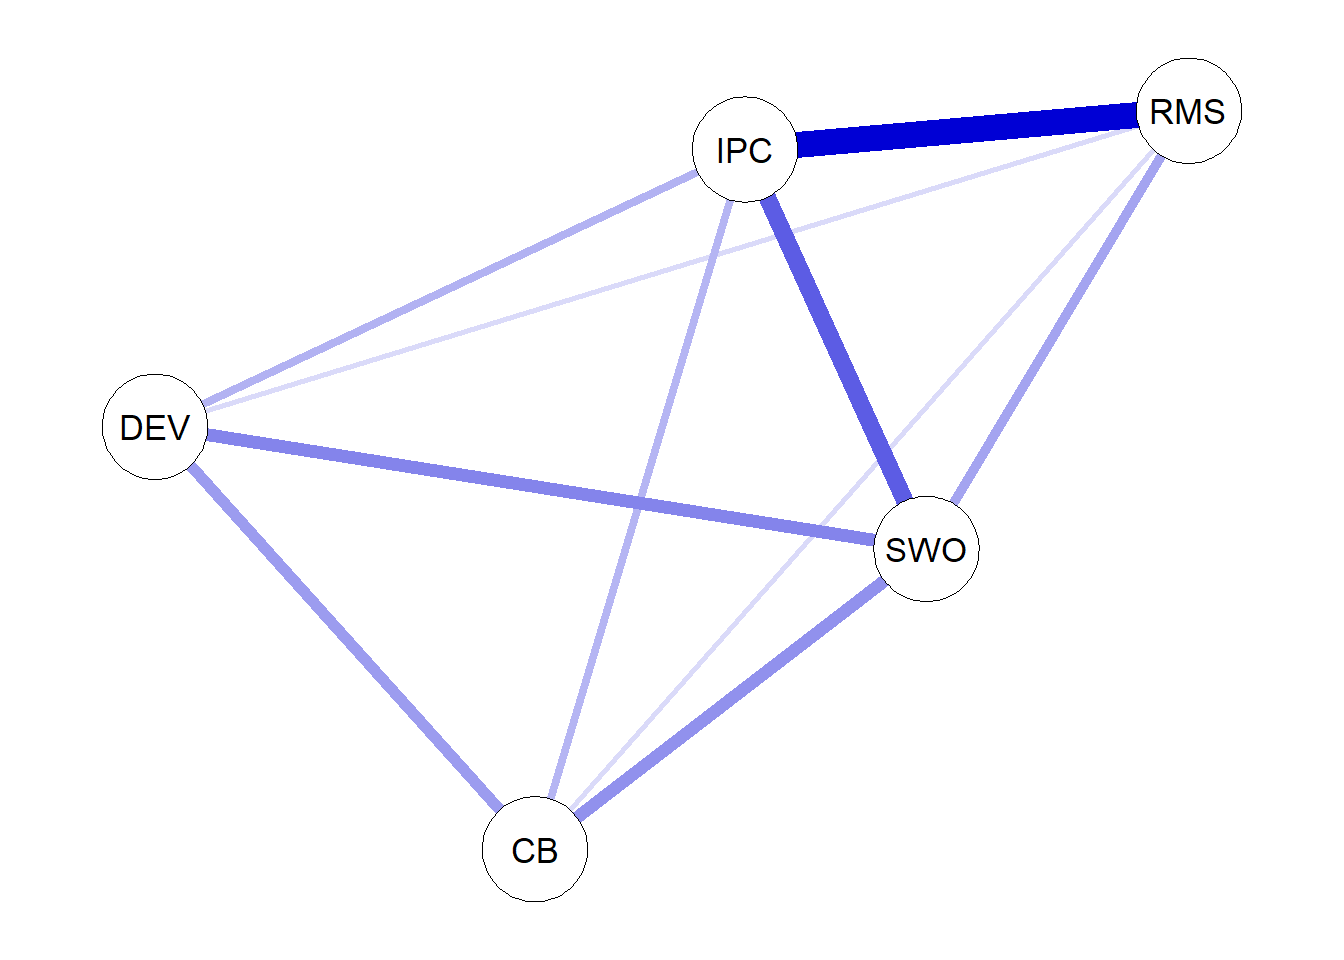
\includegraphics{2021_IDDC_Final-Report_Group-7_files/figure-latex/unnamed-chunk-4-1.pdf}

\hypertarget{work-organisational}{%
\subparagraph{Work \& Organisational}\label{work-organisational}}

\begin{Shaded}
\begin{Highlighting}[]
\CommentTok{# Create a subset for all students who have specialized in Clinical}
\NormalTok{dataWOP <-}\StringTok{ }
\StringTok{  }\NormalTok{data_wide }\OperatorTok
\StringTok{      }\KeywordTok{filter}\NormalTok{(data_wide}\OperatorTok{$}\NormalTok{Specialization }\OperatorTok{==}\StringTok{ "Spec Arbeids- en Org. Psych."}\NormalTok{)}

\CommentTok{# Estimate a network for all students who have specialized in Work & Organisational }
\NormalTok{networkWOP <-}\StringTok{ }\KeywordTok{estimateNetwork}\NormalTok{(dataWOP[,}\OperatorTok{-}\KeywordTok{c}\NormalTok{(}\DecValTok{1}\OperatorTok{:}\DecValTok{2}\NormalTok{)],}
                               \DataTypeTok{default =} \StringTok{"pcor"}\NormalTok{,}
                               \DataTypeTok{corMethod =} \StringTok{"spearman"}\NormalTok{)}

\CommentTok{# Visualize the estimated network}
\KeywordTok{qgraph}\NormalTok{(networkWOP}\OperatorTok{$}\NormalTok{graph,}
       \DataTypeTok{layout =} \StringTok{"circle"}\NormalTok{,}
       \DataTypeTok{theme =} \StringTok{"colorblind"}\NormalTok{,}
       \DataTypeTok{title.cex =} \DecValTok{2}\NormalTok{,}
       \DataTypeTok{title =} \KeywordTok{paste}\NormalTok{(}\StringTok{"Spec Arbeids- en Org. Psych.; N ="}\NormalTok{, }\KeywordTok{nrow}\NormalTok{(dataWOP))) }\CommentTok{# N = 64}
\end{Highlighting}
\end{Shaded}

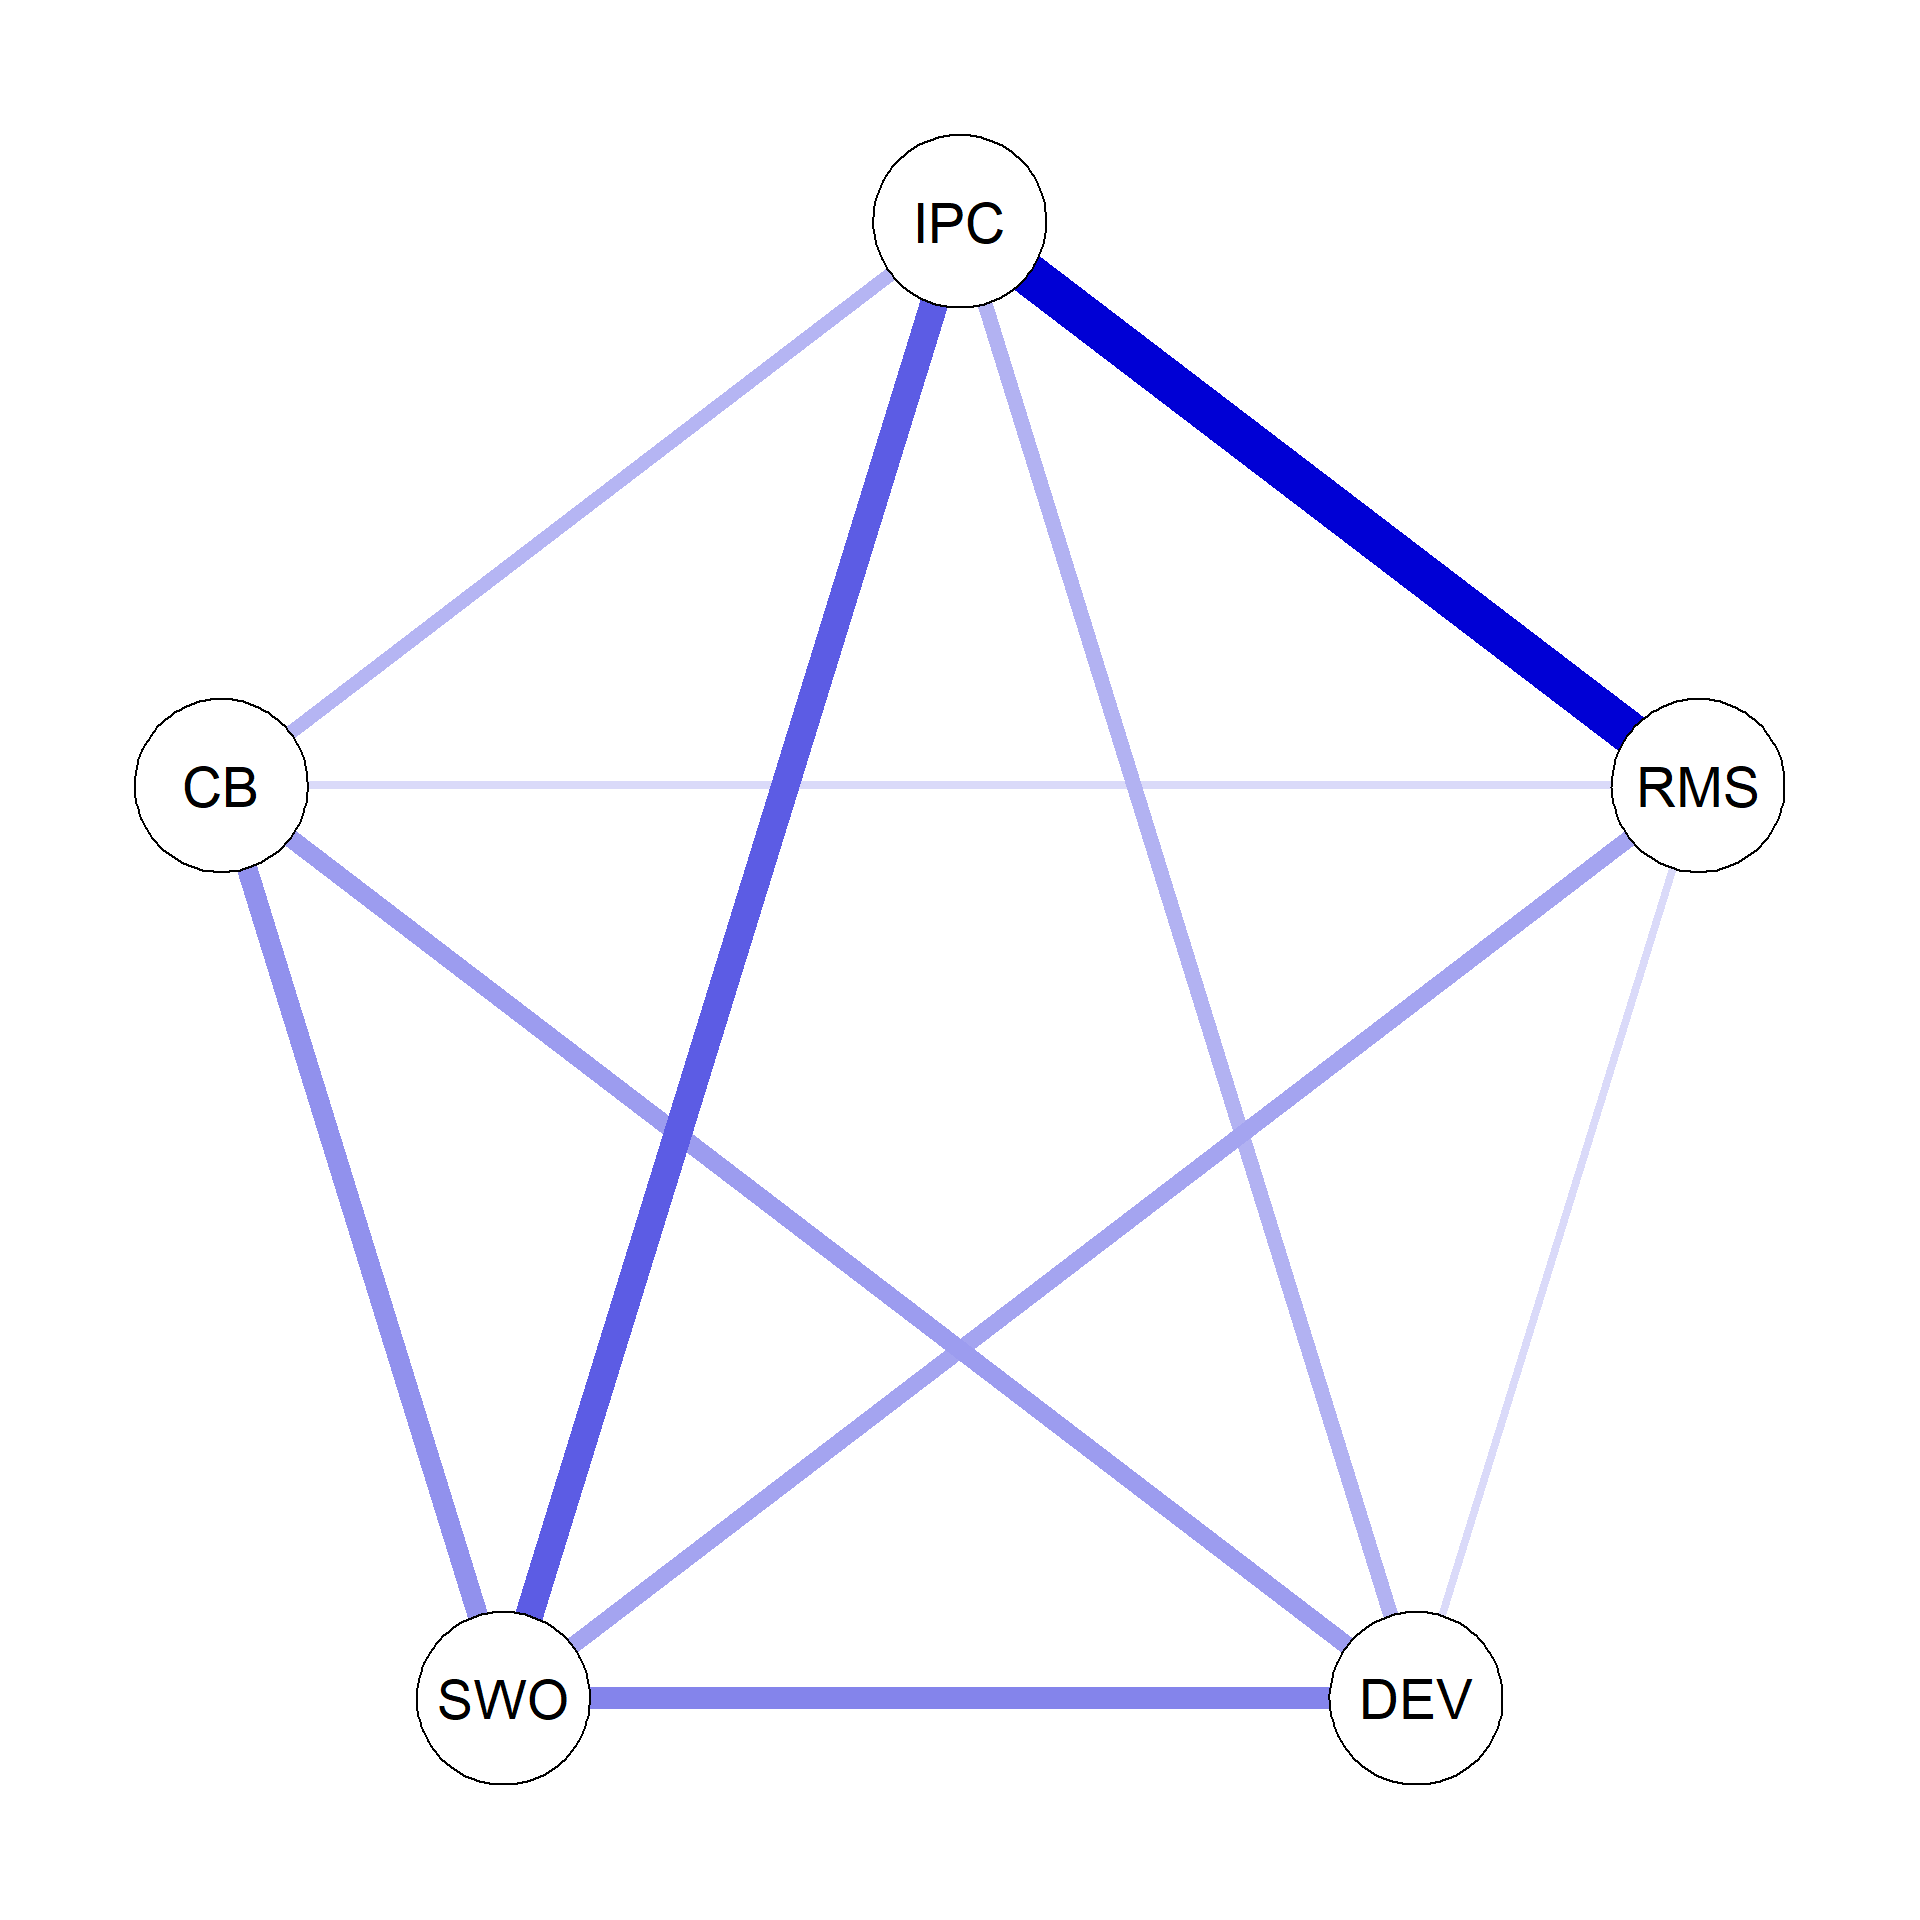
\includegraphics{2021_IDDC_Final-Report_Group-7_files/figure-latex/unnamed-chunk-5-1.pdf}

\hypertarget{social}{%
\subparagraph{Social}\label{social}}

\begin{Shaded}
\begin{Highlighting}[]
\CommentTok{# Create a subset for all students who have specialized in Social}
\NormalTok{dataSOC <-}\StringTok{ }
\StringTok{  }\NormalTok{data_wide }\OperatorTok
\StringTok{    }\KeywordTok{filter}\NormalTok{(data_wide}\OperatorTok{$}\NormalTok{Specialization }\OperatorTok{==}\StringTok{ "Spec Sociale Psychologie"}\NormalTok{)}

\CommentTok{# Estimate a network for all students who have specialized in Social}
\NormalTok{networkSOC <-}\StringTok{ }\KeywordTok{estimateNetwork}\NormalTok{(dataSOC[,}\OperatorTok{-}\KeywordTok{c}\NormalTok{(}\DecValTok{1}\OperatorTok{:}\DecValTok{2}\NormalTok{)],}
                               \DataTypeTok{default =} \StringTok{"pcor"}\NormalTok{,}
                               \DataTypeTok{corMethod =} \StringTok{"spearman"}\NormalTok{)}

\CommentTok{# Visualize the estimated network}
\KeywordTok{qgraph}\NormalTok{(networkSOC}\OperatorTok{$}\NormalTok{graph,}
       \DataTypeTok{layout =} \StringTok{"circle"}\NormalTok{,}
       \DataTypeTok{theme =} \StringTok{"colorblind"}\NormalTok{,}
       \DataTypeTok{title.cex =} \DecValTok{2}\NormalTok{,}
       \DataTypeTok{title =} \KeywordTok{paste}\NormalTok{(}\StringTok{"Spec Sociale Psychologie; N ="}\NormalTok{, }\KeywordTok{nrow}\NormalTok{(dataSOC))) }\CommentTok{# N = 56}
\end{Highlighting}
\end{Shaded}

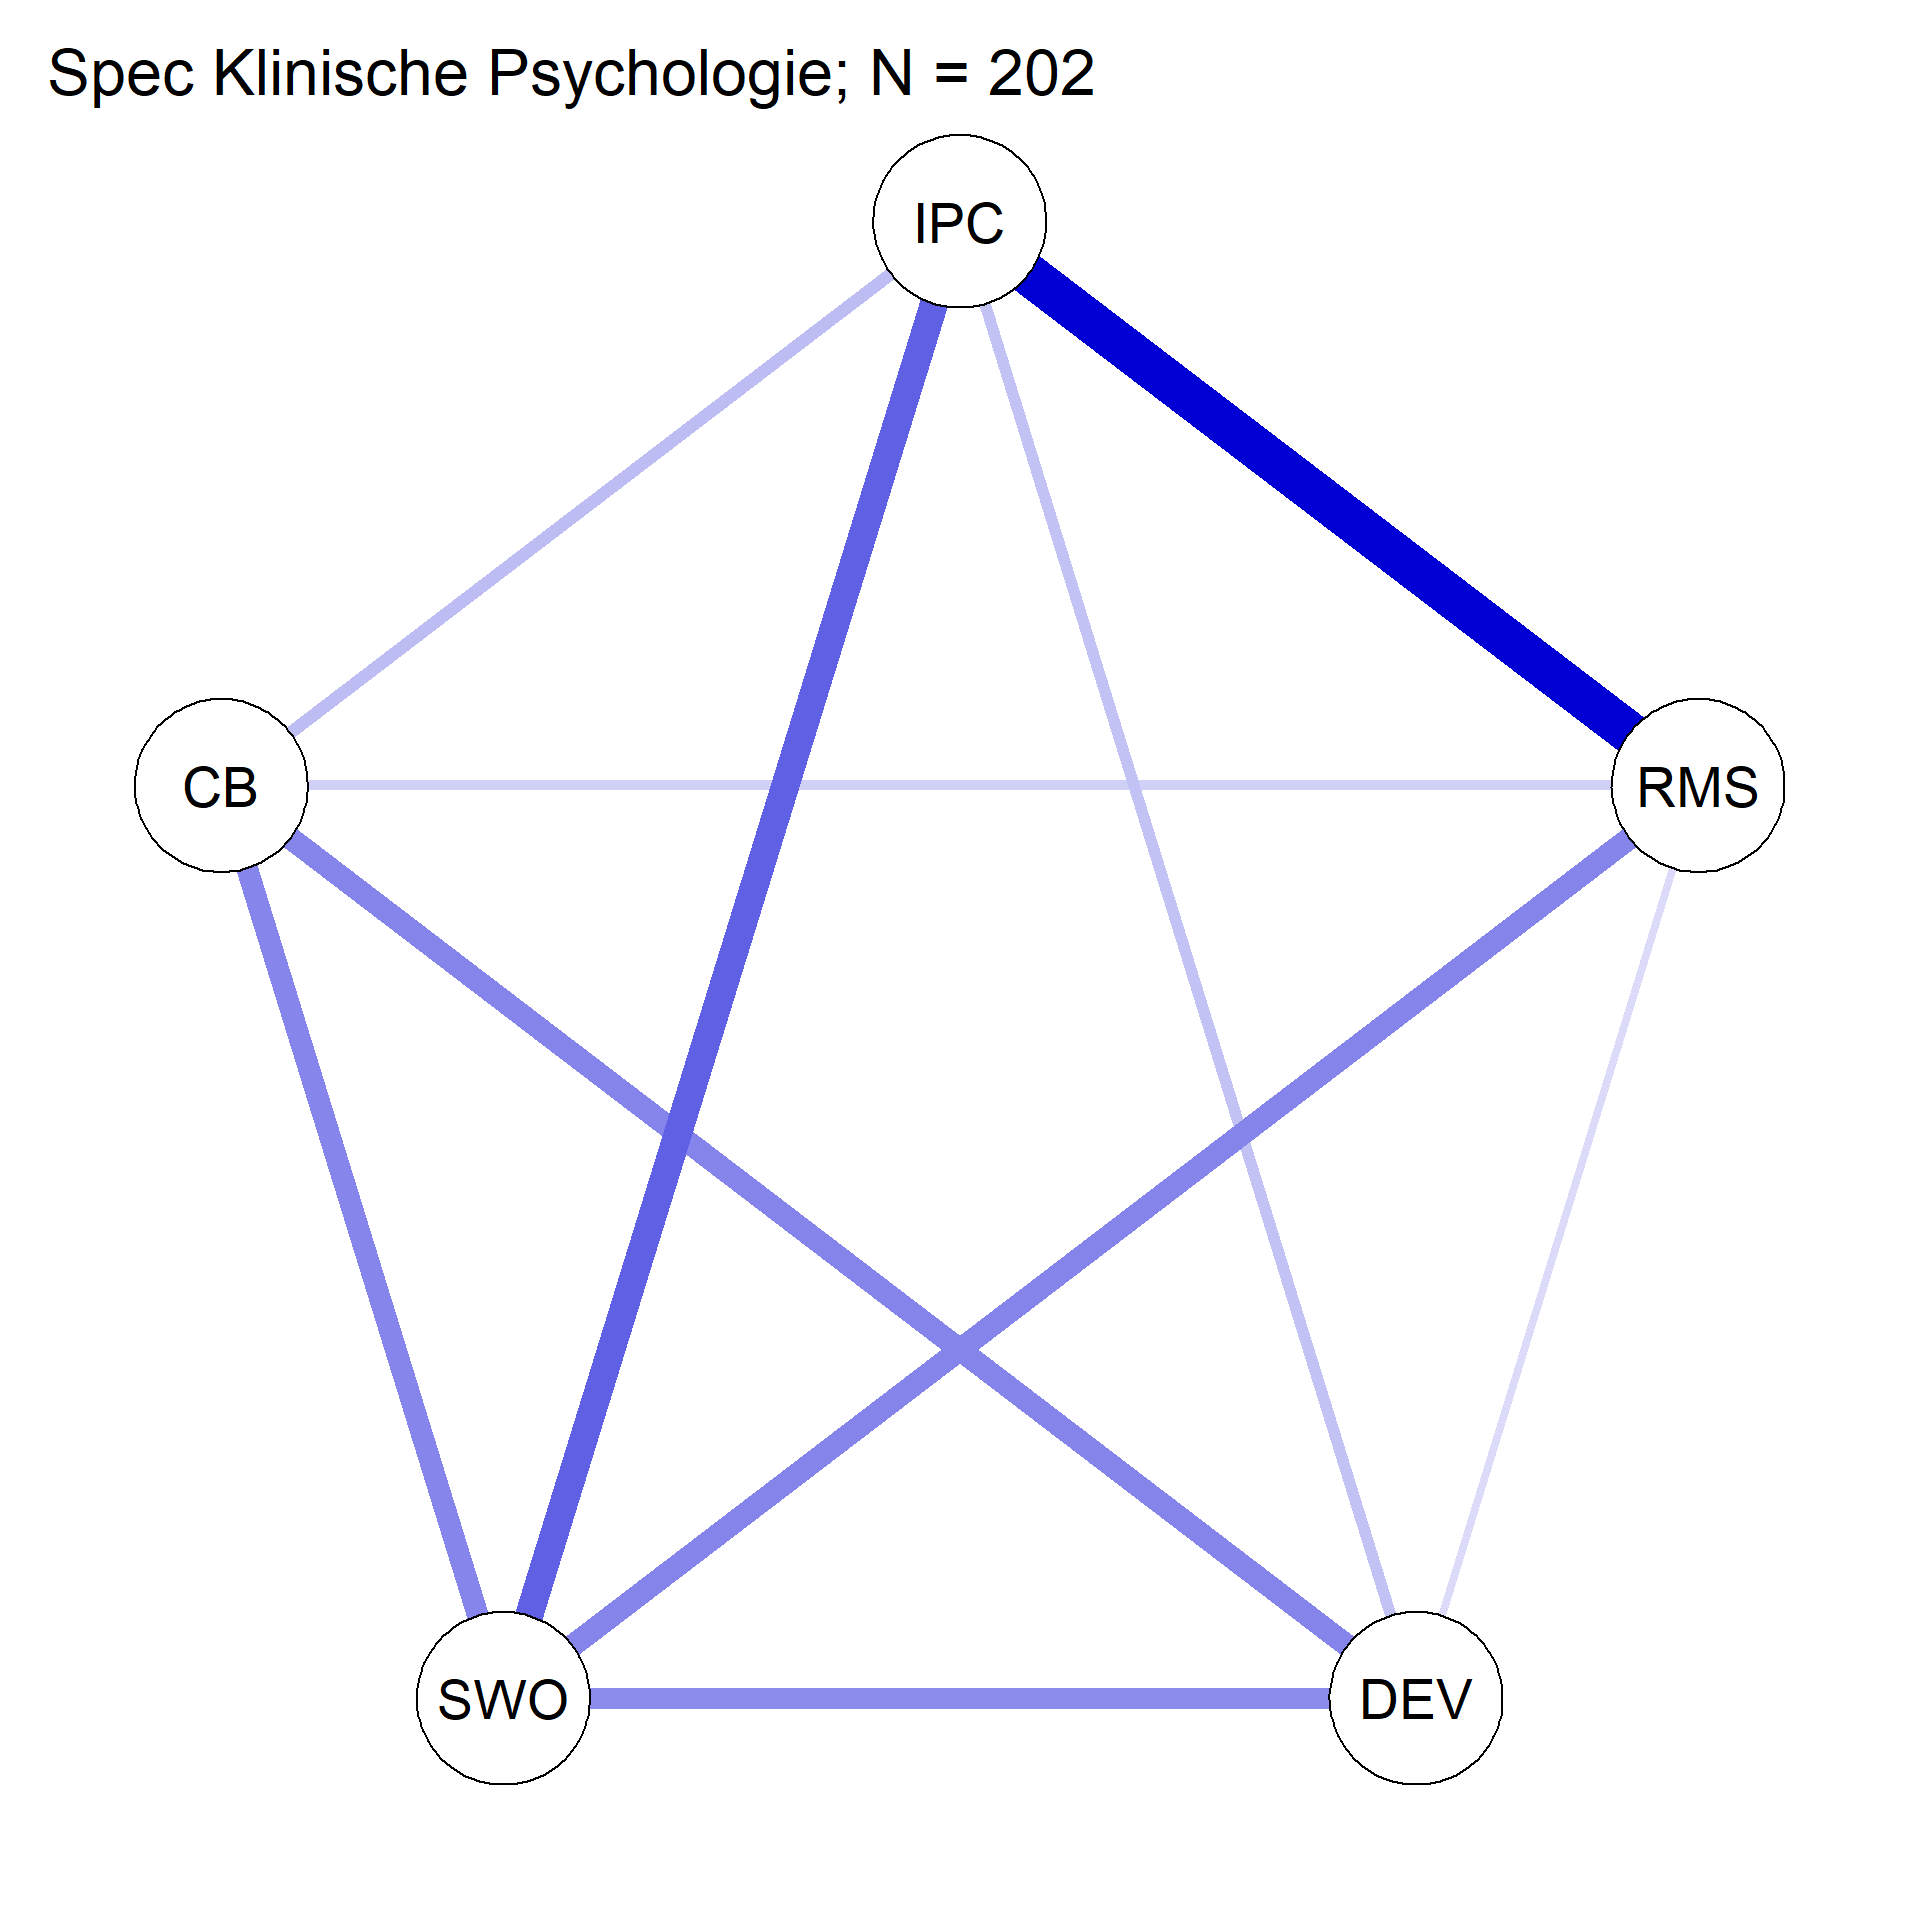
\includegraphics{2021_IDDC_Final-Report_Group-7_files/figure-latex/unnamed-chunk-6-1.pdf}

\hypertarget{brain-cognition}{%
\subparagraph{Brain \& Cognition}\label{brain-cognition}}

\begin{Shaded}
\begin{Highlighting}[]
\CommentTok{# Create a subset for all students who have specialized in Brain & Cognition}
\NormalTok{dataBC <-}\StringTok{ }
\StringTok{  }\NormalTok{data_wide }\OperatorTok
\StringTok{      }\KeywordTok{filter}\NormalTok{(data_wide}\OperatorTok{$}\NormalTok{Specialization }\OperatorTok{==}\StringTok{ "Spec Brein en Cognitie"}\NormalTok{)}

\CommentTok{# Estimate a network for all students who have specialized in Brain & Cognition}
\NormalTok{networkBC <-}\StringTok{ }\KeywordTok{estimateNetwork}\NormalTok{(dataBC[,}\OperatorTok{-}\KeywordTok{c}\NormalTok{(}\DecValTok{1}\OperatorTok{:}\DecValTok{2}\NormalTok{)],}
                               \DataTypeTok{default =} \StringTok{"pcor"}\NormalTok{,}
                               \DataTypeTok{corMethod =} \StringTok{"spearman"}\NormalTok{)}

\CommentTok{# Visualize the estimated network}
\KeywordTok{qgraph}\NormalTok{(networkBC}\OperatorTok{$}\NormalTok{graph,}
       \DataTypeTok{layout =} \StringTok{"circle"}\NormalTok{,}
       \DataTypeTok{theme =} \StringTok{"colorblind"}\NormalTok{,}
       \DataTypeTok{title.cex =} \DecValTok{2}\NormalTok{,}
       \DataTypeTok{title =} \KeywordTok{paste}\NormalTok{(}\StringTok{"Spec Brein en Cognitie; N ="}\NormalTok{, }\KeywordTok{nrow}\NormalTok{(dataBC))) }\CommentTok{# N = 40}
\end{Highlighting}
\end{Shaded}

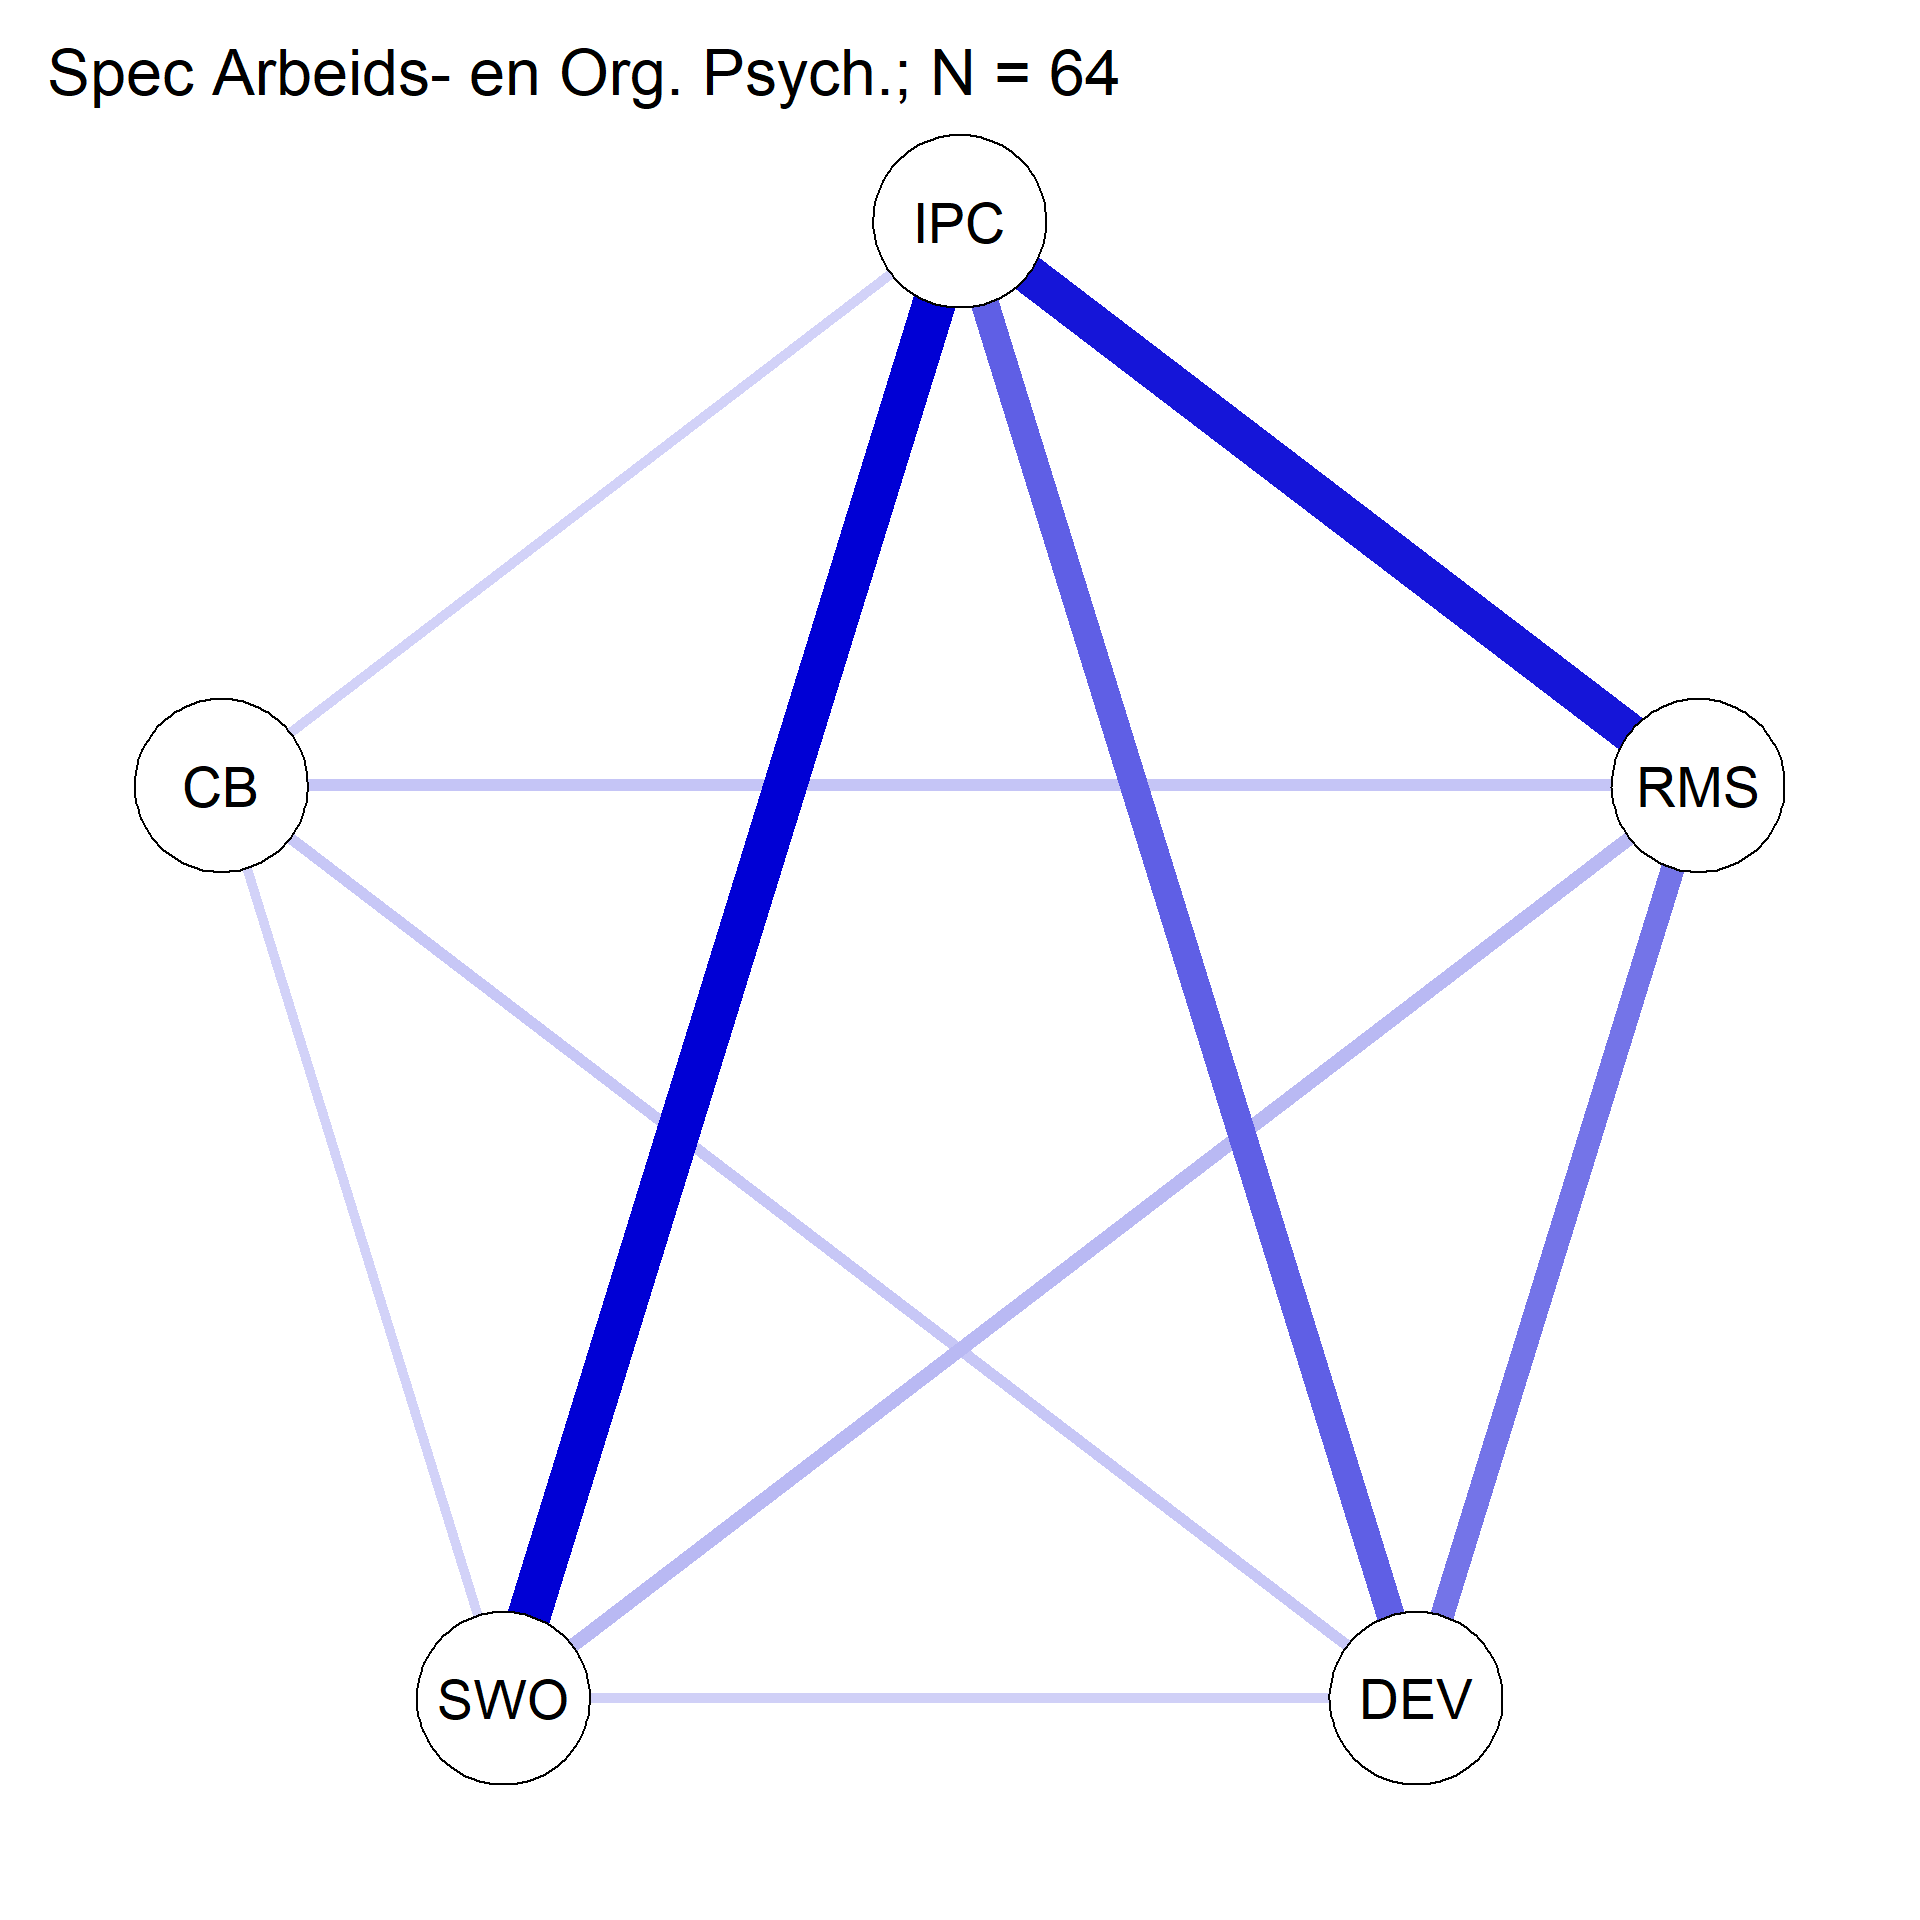
\includegraphics{2021_IDDC_Final-Report_Group-7_files/figure-latex/unnamed-chunk-7-1.pdf}

\hypertarget{clinical-dev}{%
\subparagraph{Clinical Dev}\label{clinical-dev}}

\begin{Shaded}
\begin{Highlighting}[]
\CommentTok{# Create a subset for all students who have specialized in Clinical Development}
\NormalTok{dataDEV <-}\StringTok{ }
\StringTok{  }\NormalTok{data_wide }\OperatorTok
\StringTok{      }\KeywordTok{filter}\NormalTok{(data_wide}\OperatorTok{$}\NormalTok{Specialization }\OperatorTok{==}\StringTok{ "Spec Klinische Ontwikkelingsps"}\NormalTok{)}

\CommentTok{# Estimate a network for all students who have specialized in Clinical Developmental}
\NormalTok{networkDEV <-}\StringTok{ }\KeywordTok{estimateNetwork}\NormalTok{(dataDEV[,}\OperatorTok{-}\KeywordTok{c}\NormalTok{(}\DecValTok{1}\OperatorTok{:}\DecValTok{2}\NormalTok{)],}
                               \DataTypeTok{default =} \StringTok{"pcor"}\NormalTok{,}
                               \DataTypeTok{corMethod =} \StringTok{"spearman"}\NormalTok{)}

\CommentTok{# Visualize the estimated network}
\KeywordTok{qgraph}\NormalTok{(networkDEV}\OperatorTok{$}\NormalTok{graph,}
       \DataTypeTok{layout =} \StringTok{"circle"}\NormalTok{,}
       \DataTypeTok{theme =} \StringTok{"colorblind"}\NormalTok{,}
       \DataTypeTok{title.cex =} \DecValTok{2}\NormalTok{,}
       \DataTypeTok{title =} \KeywordTok{paste}\NormalTok{(}\StringTok{"Spec Klinische Ontwikkelingsps; N ="}\NormalTok{, }\KeywordTok{nrow}\NormalTok{(dataDEV))) }\CommentTok{# N = 50}
\end{Highlighting}
\end{Shaded}

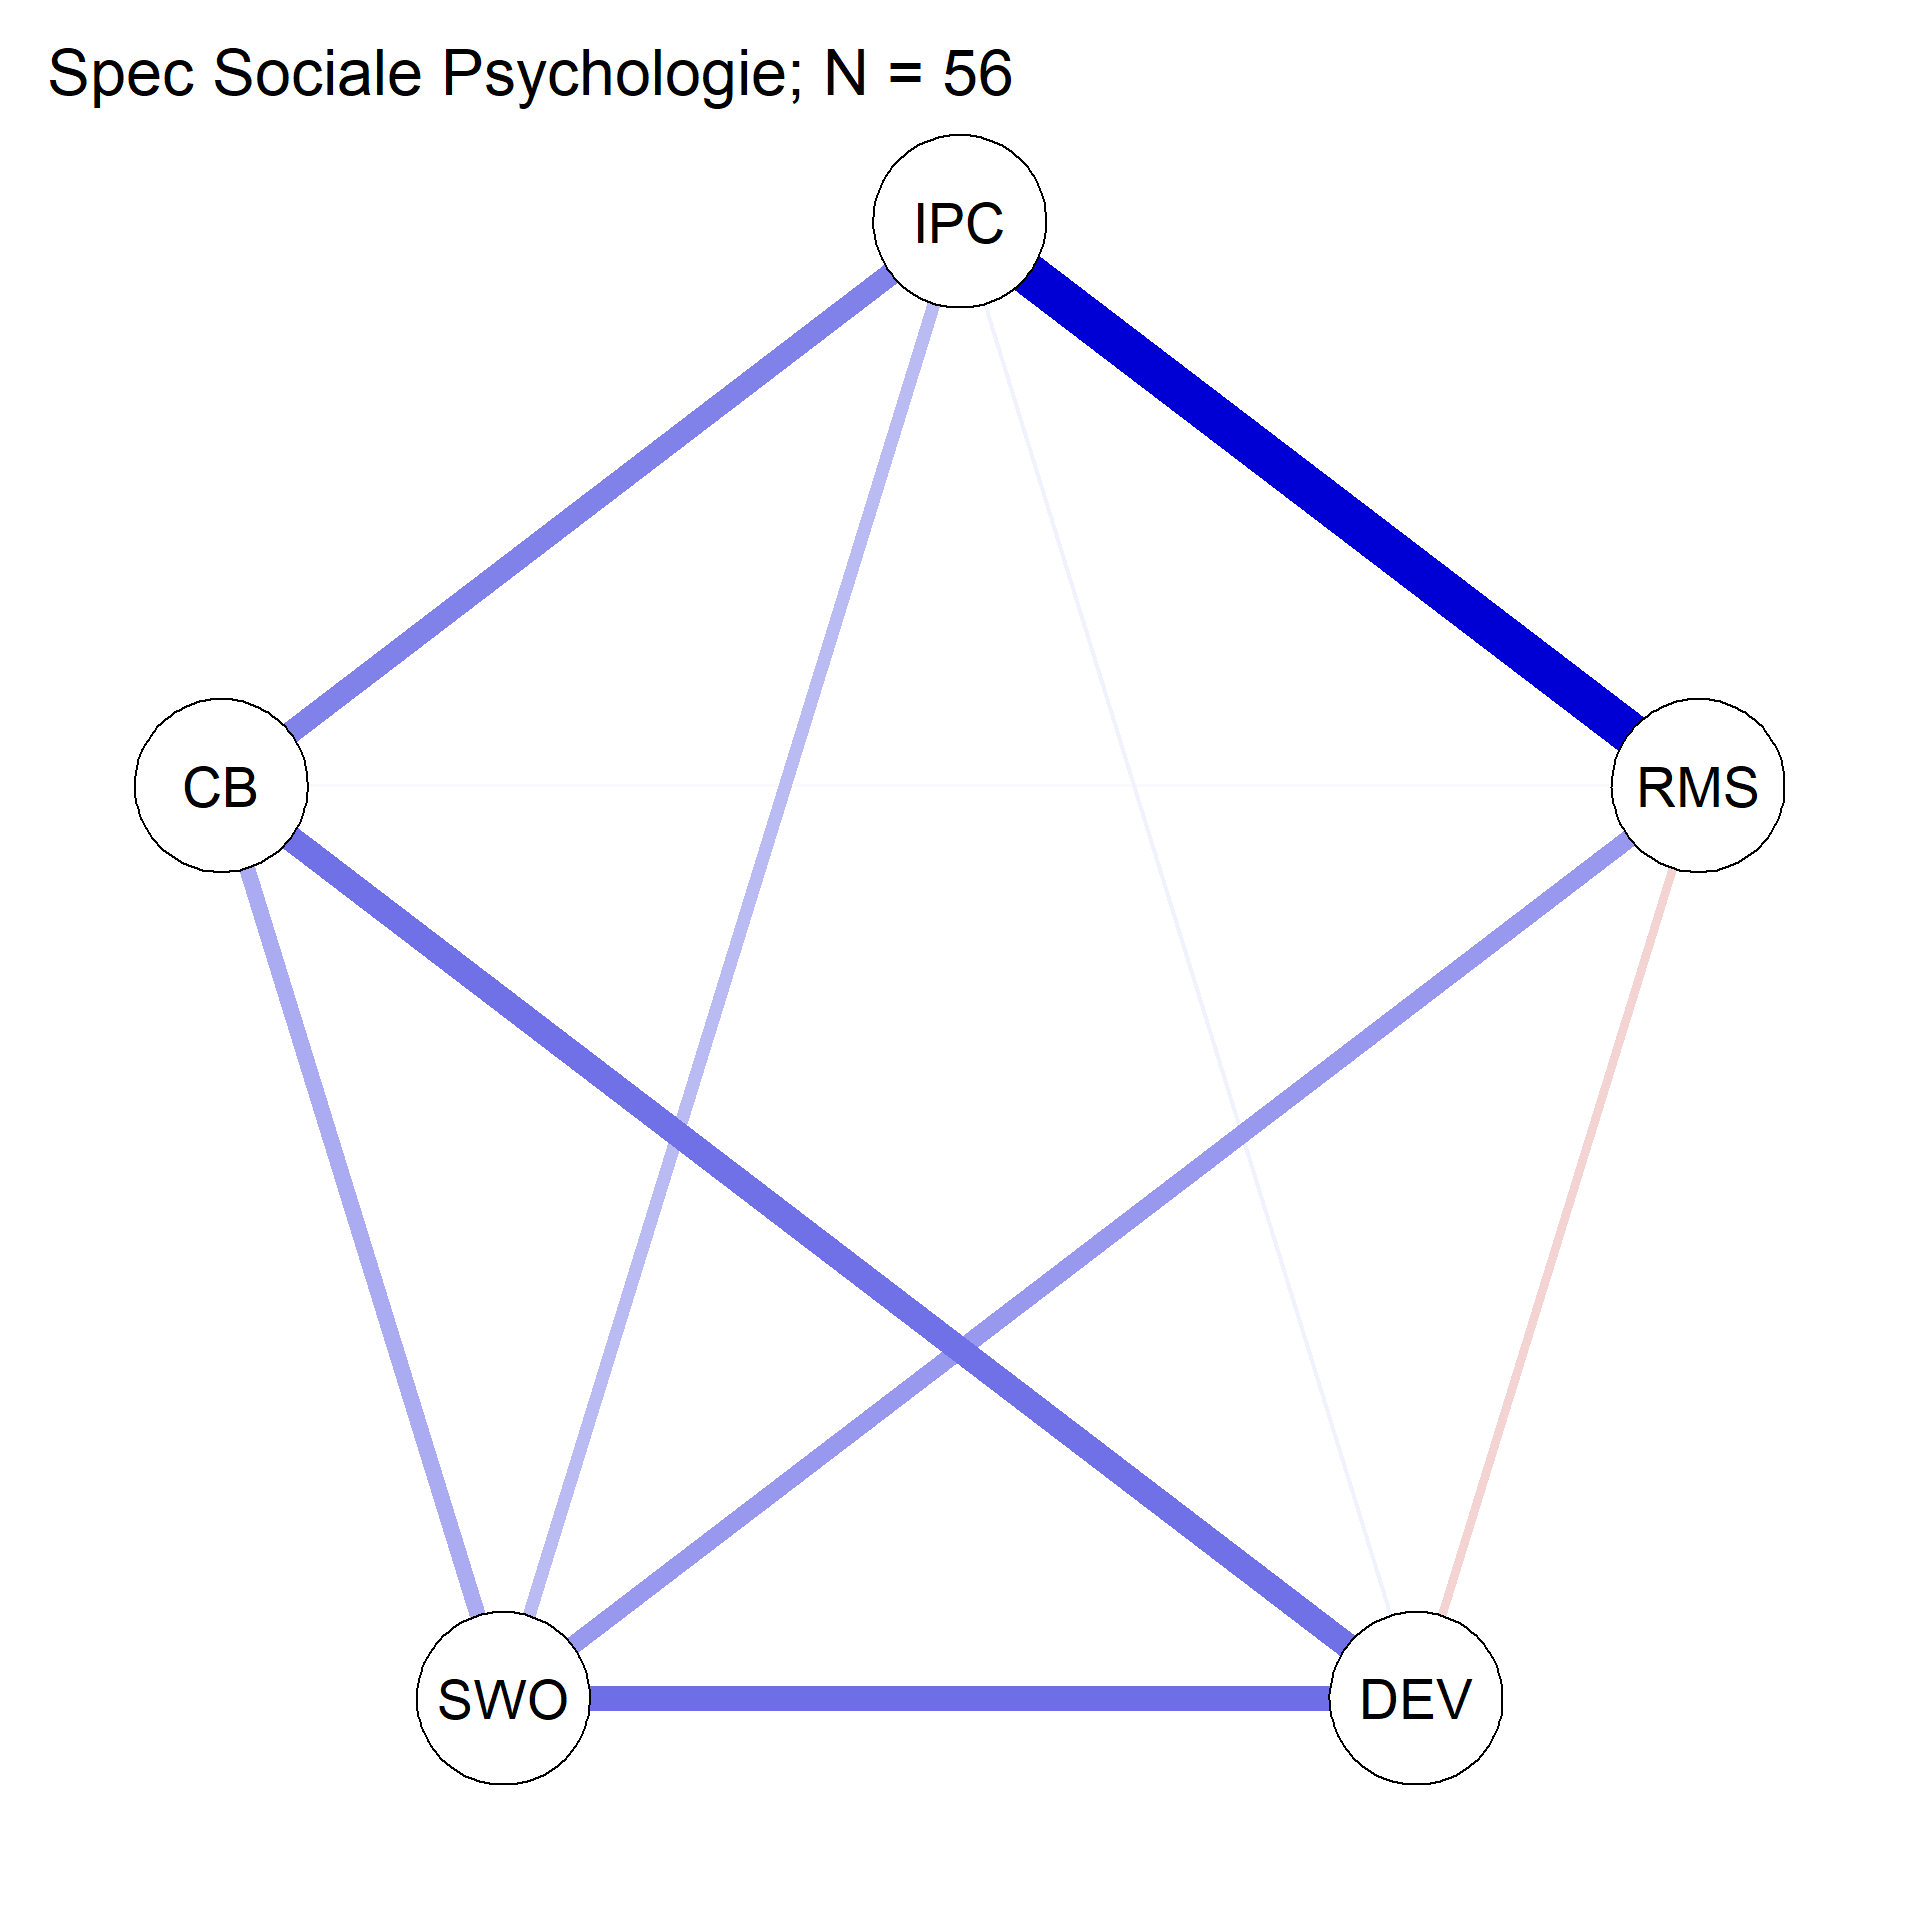
\includegraphics{2021_IDDC_Final-Report_Group-7_files/figure-latex/unnamed-chunk-8-1.pdf}

\hypertarget{clinical-neuro}{%
\subparagraph{Clinical Neuro}\label{clinical-neuro}}

\begin{Shaded}
\begin{Highlighting}[]
\CommentTok{# Create a subset for all students who have specialized in Clinical Neuro}
\NormalTok{dataCNP <-}\StringTok{ }
\StringTok{  }\NormalTok{data_wide }\OperatorTok
\StringTok{      }\KeywordTok{filter}\NormalTok{(data_wide}\OperatorTok{$}\NormalTok{Specialization }\OperatorTok{==}\StringTok{ "Spec Klinische Neuropsych."}\NormalTok{)}

\CommentTok{# Estimate a network for all students who have specialized in Clinical Neuro}
\NormalTok{networkCNP <-}\StringTok{ }\KeywordTok{estimateNetwork}\NormalTok{(dataCNP[,}\OperatorTok{-}\KeywordTok{c}\NormalTok{(}\DecValTok{1}\OperatorTok{:}\DecValTok{2}\NormalTok{)],}
                               \DataTypeTok{default =} \StringTok{"pcor"}\NormalTok{,}
                               \DataTypeTok{corMethod =} \StringTok{"spearman"}\NormalTok{)}

\CommentTok{# Visualize the estimated network}
\KeywordTok{qgraph}\NormalTok{(networkCNP}\OperatorTok{$}\NormalTok{graph,}
       \DataTypeTok{layout =} \StringTok{"circle"}\NormalTok{,}
       \DataTypeTok{theme =} \StringTok{"colorblind"}\NormalTok{,}
       \DataTypeTok{title.cex =} \DecValTok{2}\NormalTok{,}
       \DataTypeTok{title =} \KeywordTok{paste}\NormalTok{(}\StringTok{"Spec Klinische Neuropsych.    ; N ="}\NormalTok{, }\KeywordTok{nrow}\NormalTok{(dataCNP))) }\CommentTok{# N = 22}
\end{Highlighting}
\end{Shaded}

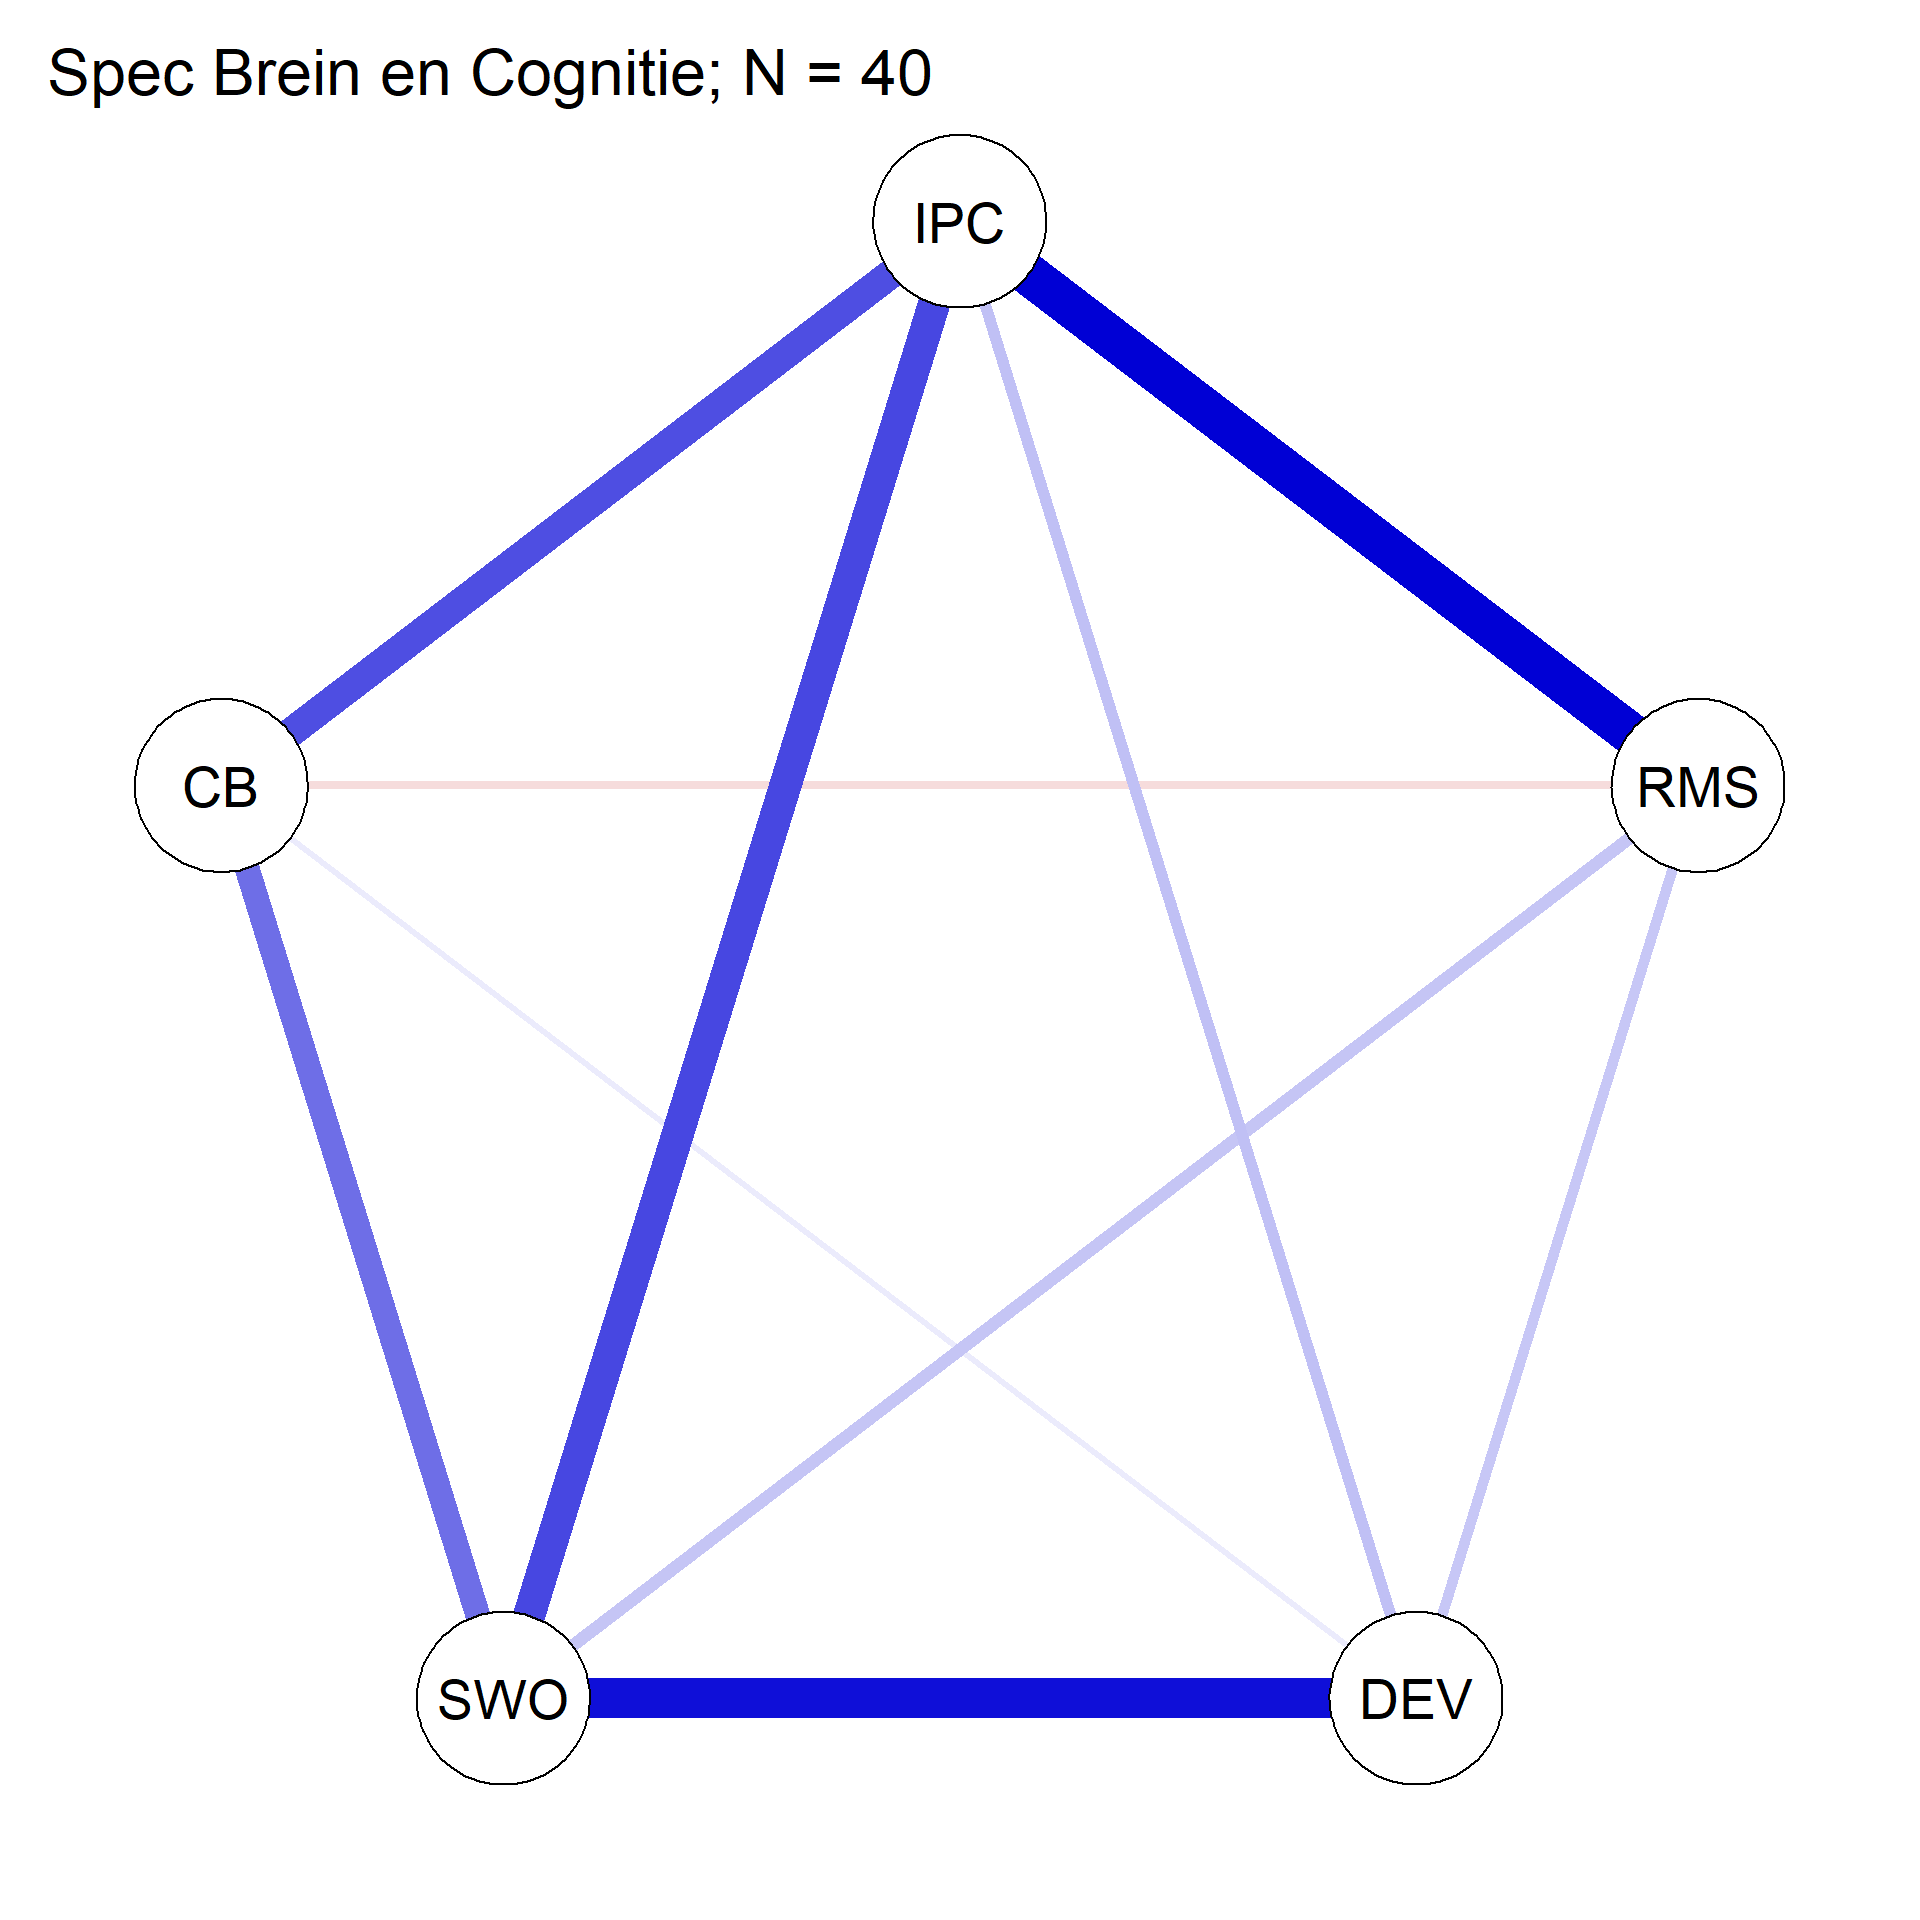
\includegraphics{2021_IDDC_Final-Report_Group-7_files/figure-latex/unnamed-chunk-9-1.pdf}

\hypertarget{methods}{%
\subparagraph{Methods}\label{methods}}

\begin{Shaded}
\begin{Highlighting}[]
\CommentTok{# Create a subset for all students who have specialized in Methods}
\NormalTok{dataPML <-}\StringTok{ }
\StringTok{  }\NormalTok{data_wide }\OperatorTok
\StringTok{      }\KeywordTok{filter}\NormalTok{(data_wide}\OperatorTok{$}\NormalTok{Specialization }\OperatorTok{==}\StringTok{ "Spec Psych. Methodenleer"}\NormalTok{)}

\CommentTok{# Estimate a network for all students who have specialized in Methods}
\NormalTok{networkPML <-}\StringTok{ }\KeywordTok{estimateNetwork}\NormalTok{(dataPML[,}\OperatorTok{-}\KeywordTok{c}\NormalTok{(}\DecValTok{1}\OperatorTok{:}\DecValTok{2}\NormalTok{)],}
                               \DataTypeTok{default =} \StringTok{"pcor"}\NormalTok{,}
                               \DataTypeTok{corMethod =} \StringTok{"spearman"}\NormalTok{)}

\CommentTok{# Visualize the estimated network}
\KeywordTok{qgraph}\NormalTok{(networkPML}\OperatorTok{$}\NormalTok{graph,}
       \DataTypeTok{layout =} \StringTok{"circle"}\NormalTok{,}
       \DataTypeTok{theme =} \StringTok{"colorblind"}\NormalTok{,}
       \DataTypeTok{title.cex =} \DecValTok{2}\NormalTok{,}
       \DataTypeTok{title =} \KeywordTok{paste}\NormalTok{(}\StringTok{"Spec Psych. Methodenleer; N ="}\NormalTok{, }\KeywordTok{nrow}\NormalTok{(dataPML))) }\CommentTok{# N = 31}
\end{Highlighting}
\end{Shaded}

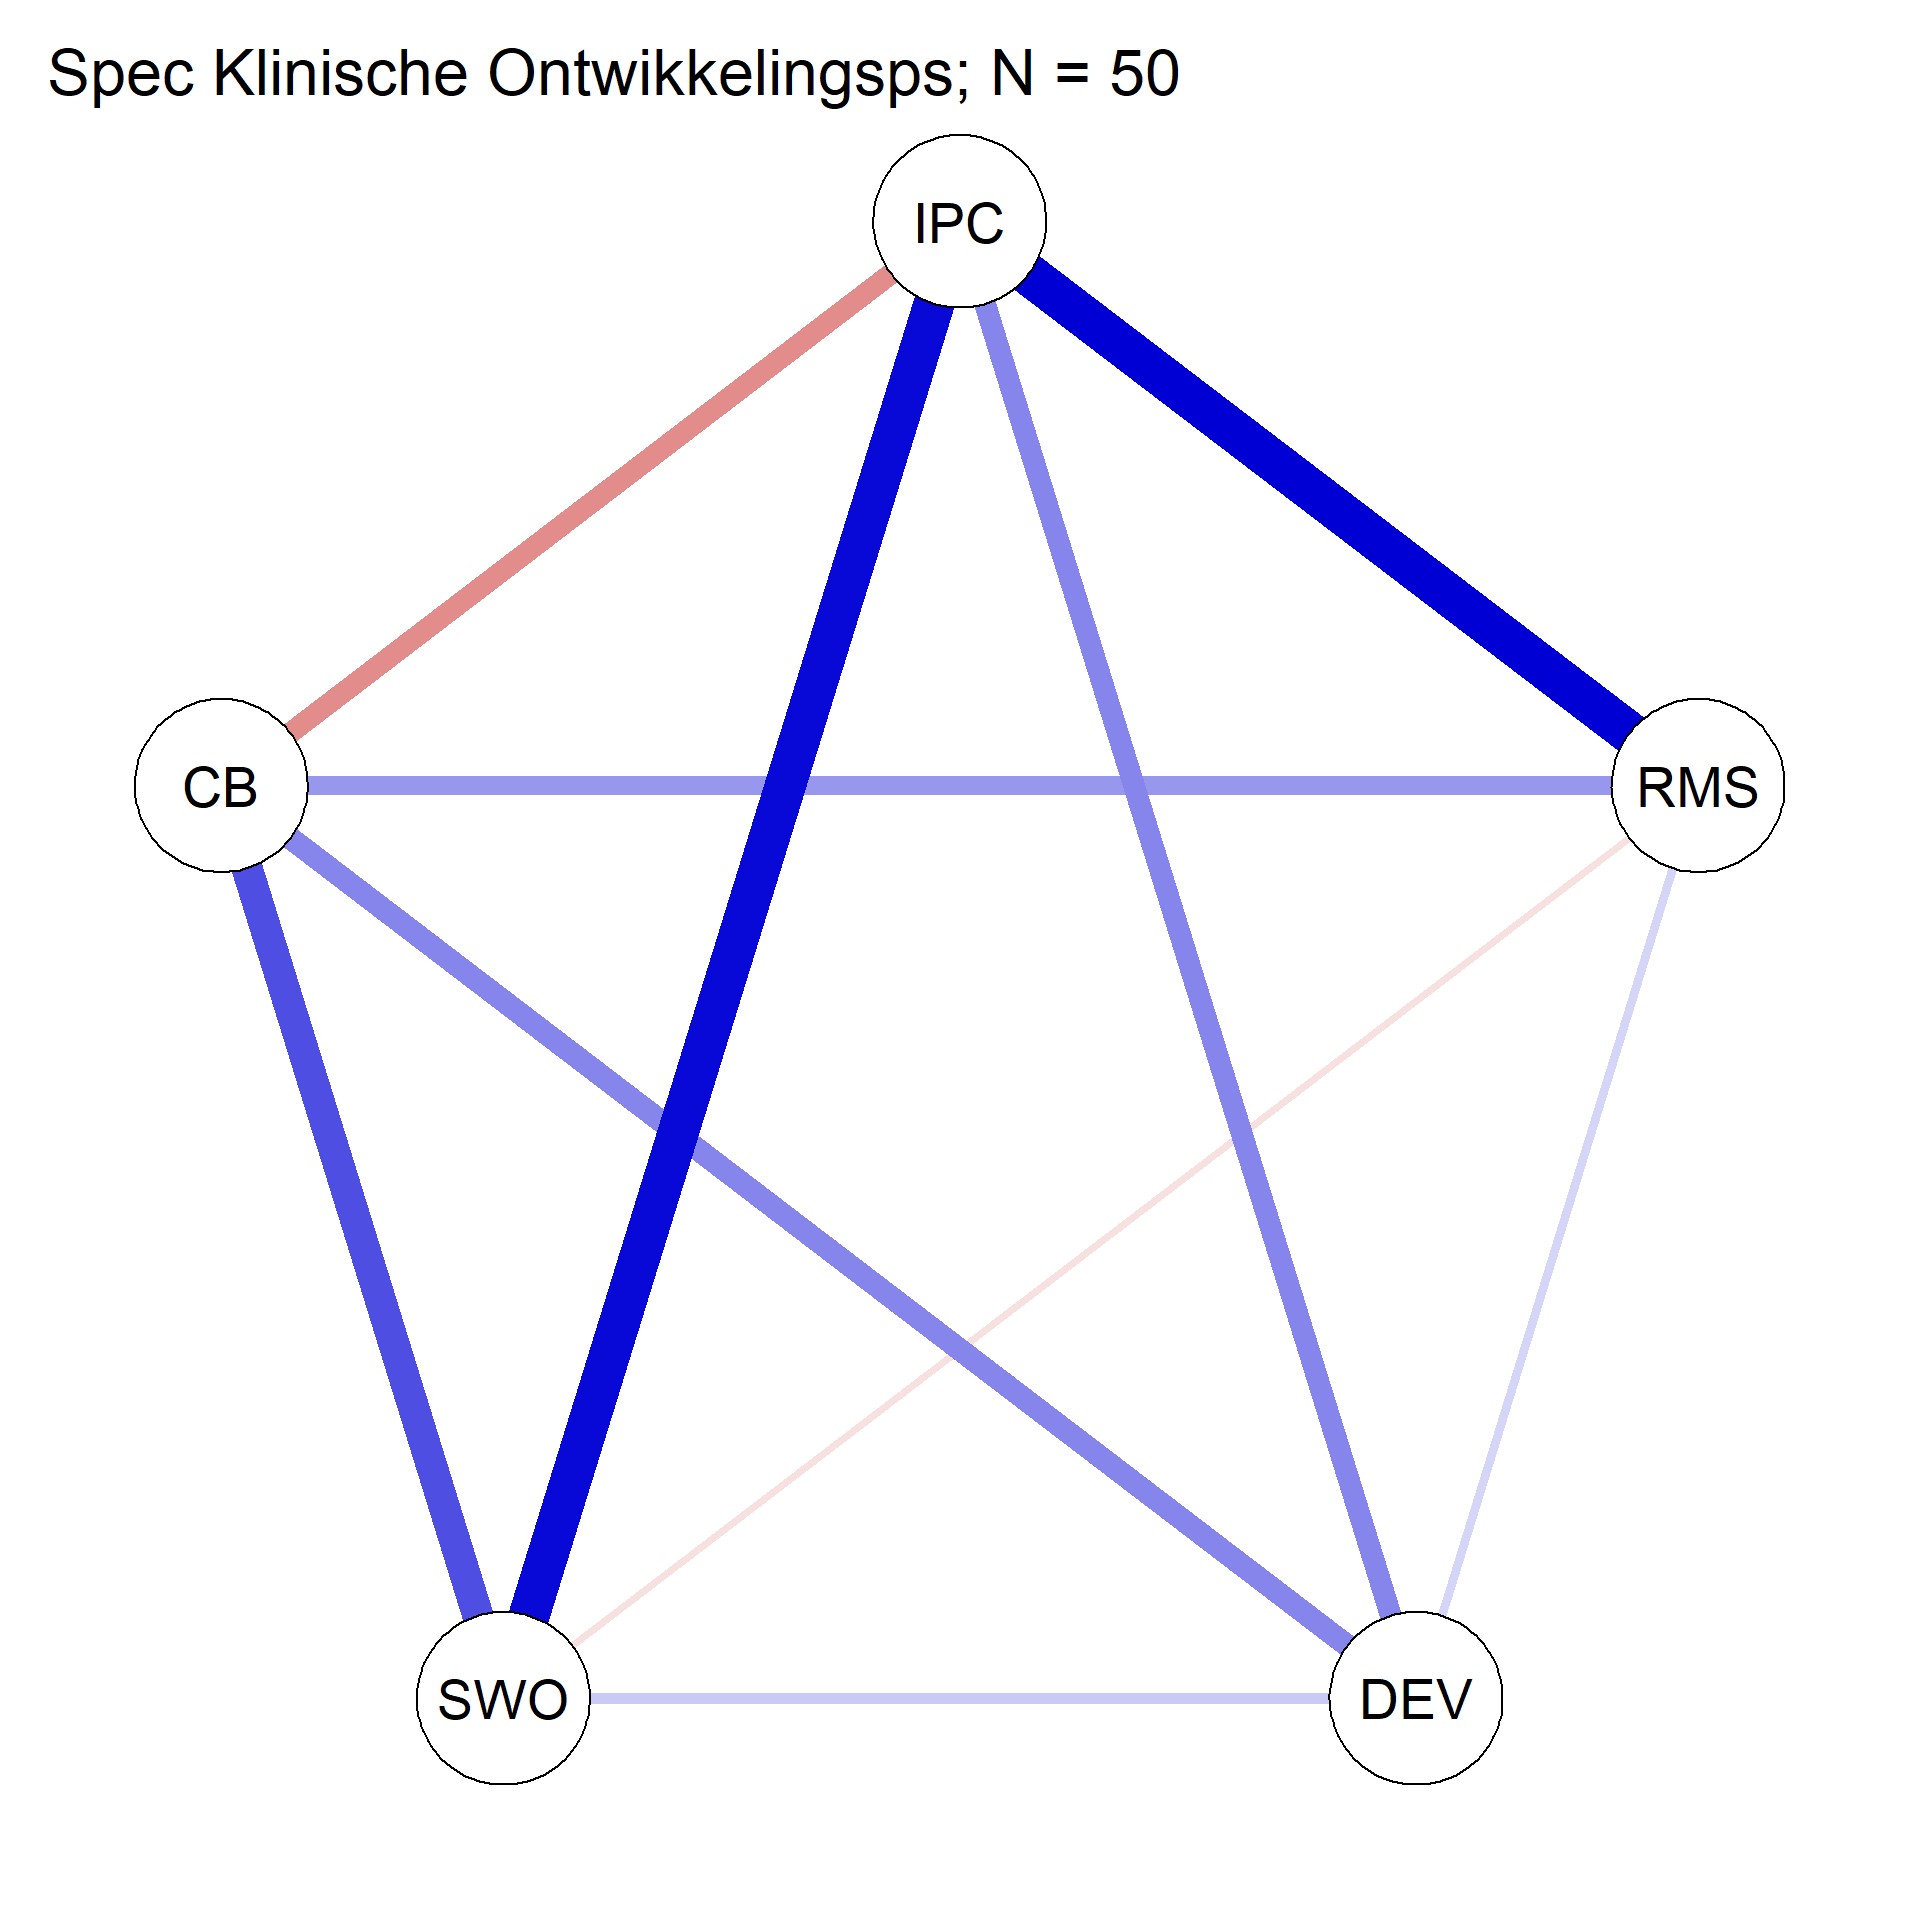
\includegraphics{2021_IDDC_Final-Report_Group-7_files/figure-latex/unnamed-chunk-10-1.pdf}

\hypertarget{estimating-a-network-for-every-specialization-using-a-dummy-yesno}{%
\paragraph{Estimating a network for every specialization using a dummy
(Yes/No)}\label{estimating-a-network-for-every-specialization-using-a-dummy-yesno}}

\hypertarget{clinical-1}{%
\subparagraph{Clinical}\label{clinical-1}}

\begin{Shaded}
\begin{Highlighting}[]
\CommentTok{# Create Dummy Variable for "CLIN" Specialization: Yes/No}
\NormalTok{dataCLIN <-}\StringTok{ }
\StringTok{  }\NormalTok{data_wide }\OperatorTok
\StringTok{      }\KeywordTok{mutate}\NormalTok{(}\DataTypeTok{CLIN =} \KeywordTok{ifelse}\NormalTok{(data_wide}\OperatorTok{$}\NormalTok{Specialization }\OperatorTok{==}\StringTok{ "Spec Klinische Psychologie"}\NormalTok{, }\DecValTok{1}\NormalTok{, }\DecValTok{0}\NormalTok{))}


\NormalTok{networkCLIN <-}\StringTok{ }\KeywordTok{estimateNetwork}\NormalTok{(dataCLIN[,}\OperatorTok{-}\KeywordTok{c}\NormalTok{(}\DecValTok{1}\OperatorTok{:}\DecValTok{2}\NormalTok{)],}
                               \DataTypeTok{default =} \StringTok{"pcor"}\NormalTok{,}
                               \DataTypeTok{corMethod =} \StringTok{"spearman"}\NormalTok{)}

\KeywordTok{qgraph}\NormalTok{(networkCLIN}\OperatorTok{$}\NormalTok{graph,}
       \DataTypeTok{layout =} \StringTok{"circle"}\NormalTok{,}
       \DataTypeTok{theme =} \StringTok{"colorblind"}\NormalTok{,}
       \DataTypeTok{title.cex =} \DecValTok{2}\NormalTok{,}
       \DataTypeTok{title =} \KeywordTok{paste}\NormalTok{(}\StringTok{"Spec Klinische Psychologie (Yes/No); N ="}\NormalTok{, }\KeywordTok{nrow}\NormalTok{(dataCLIN)))}
\end{Highlighting}
\end{Shaded}

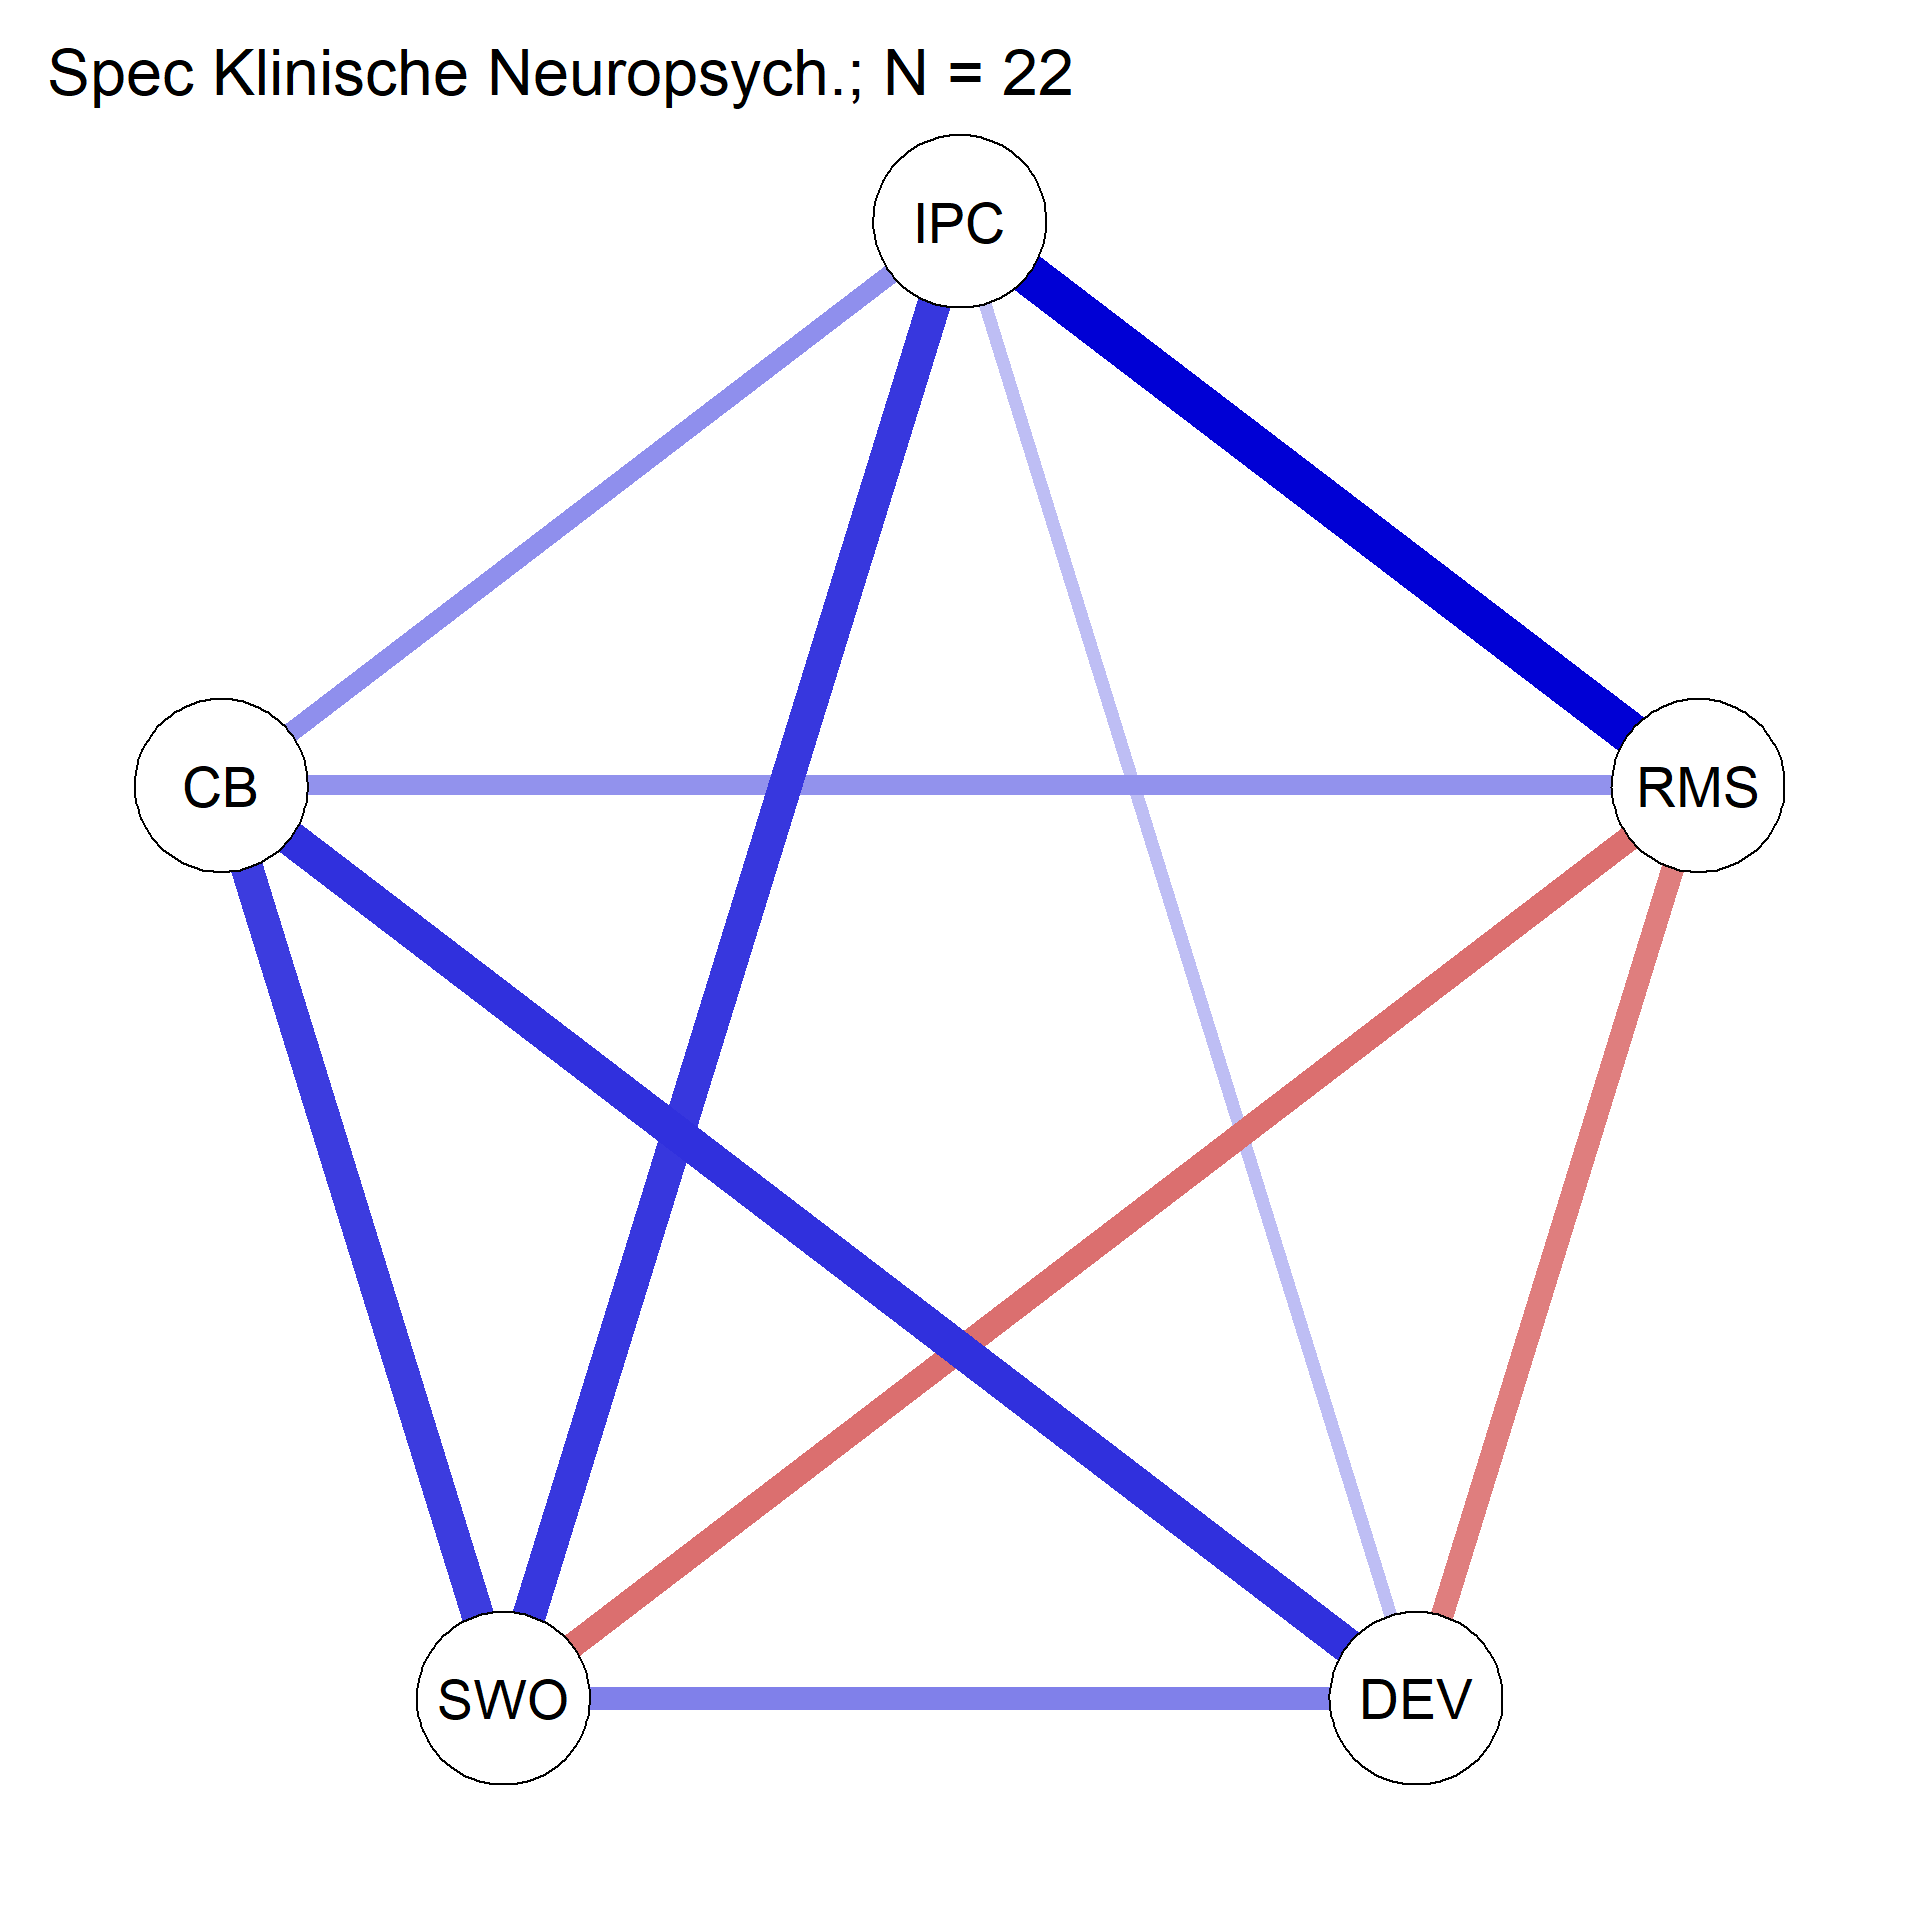
\includegraphics{2021_IDDC_Final-Report_Group-7_files/figure-latex/unnamed-chunk-11-1.pdf}

\hypertarget{work-organisational-1}{%
\subparagraph{Work \& Organisational}\label{work-organisational-1}}

\begin{Shaded}
\begin{Highlighting}[]
\CommentTok{# Create Dummy Variable for "WOP" Specialization: Yes/No}
\NormalTok{dataWOP <-}\StringTok{ }
\StringTok{  }\NormalTok{data_wide }\OperatorTok
\StringTok{      }\KeywordTok{mutate}\NormalTok{(}\DataTypeTok{WOP =} \KeywordTok{ifelse}\NormalTok{(data_wide}\OperatorTok{$}\NormalTok{Specialization }\OperatorTok{==}\StringTok{ "Spec Arbeids- en Org. Psych."}\NormalTok{, }\DecValTok{1}\NormalTok{, }\DecValTok{0}\NormalTok{))}


\NormalTok{networkWOP <-}\StringTok{ }\KeywordTok{estimateNetwork}\NormalTok{(dataWOP[,}\OperatorTok{-}\KeywordTok{c}\NormalTok{(}\DecValTok{1}\OperatorTok{:}\DecValTok{2}\NormalTok{)],}
                               \DataTypeTok{default =} \StringTok{"pcor"}\NormalTok{,}
                               \DataTypeTok{corMethod =} \StringTok{"spearman"}\NormalTok{)}

\KeywordTok{qgraph}\NormalTok{(networkWOP}\OperatorTok{$}\NormalTok{graph,}
       \DataTypeTok{layout =} \StringTok{"circle"}\NormalTok{,}
       \DataTypeTok{theme =} \StringTok{"colorblind"}\NormalTok{,}
       \DataTypeTok{title.cex =} \DecValTok{2}\NormalTok{,}
       \DataTypeTok{title =} \KeywordTok{paste}\NormalTok{(}\StringTok{"Spec Arbeids- en Org. Psych. (Yes/No); N ="}\NormalTok{, }\KeywordTok{nrow}\NormalTok{(dataWOP)))}
\end{Highlighting}
\end{Shaded}

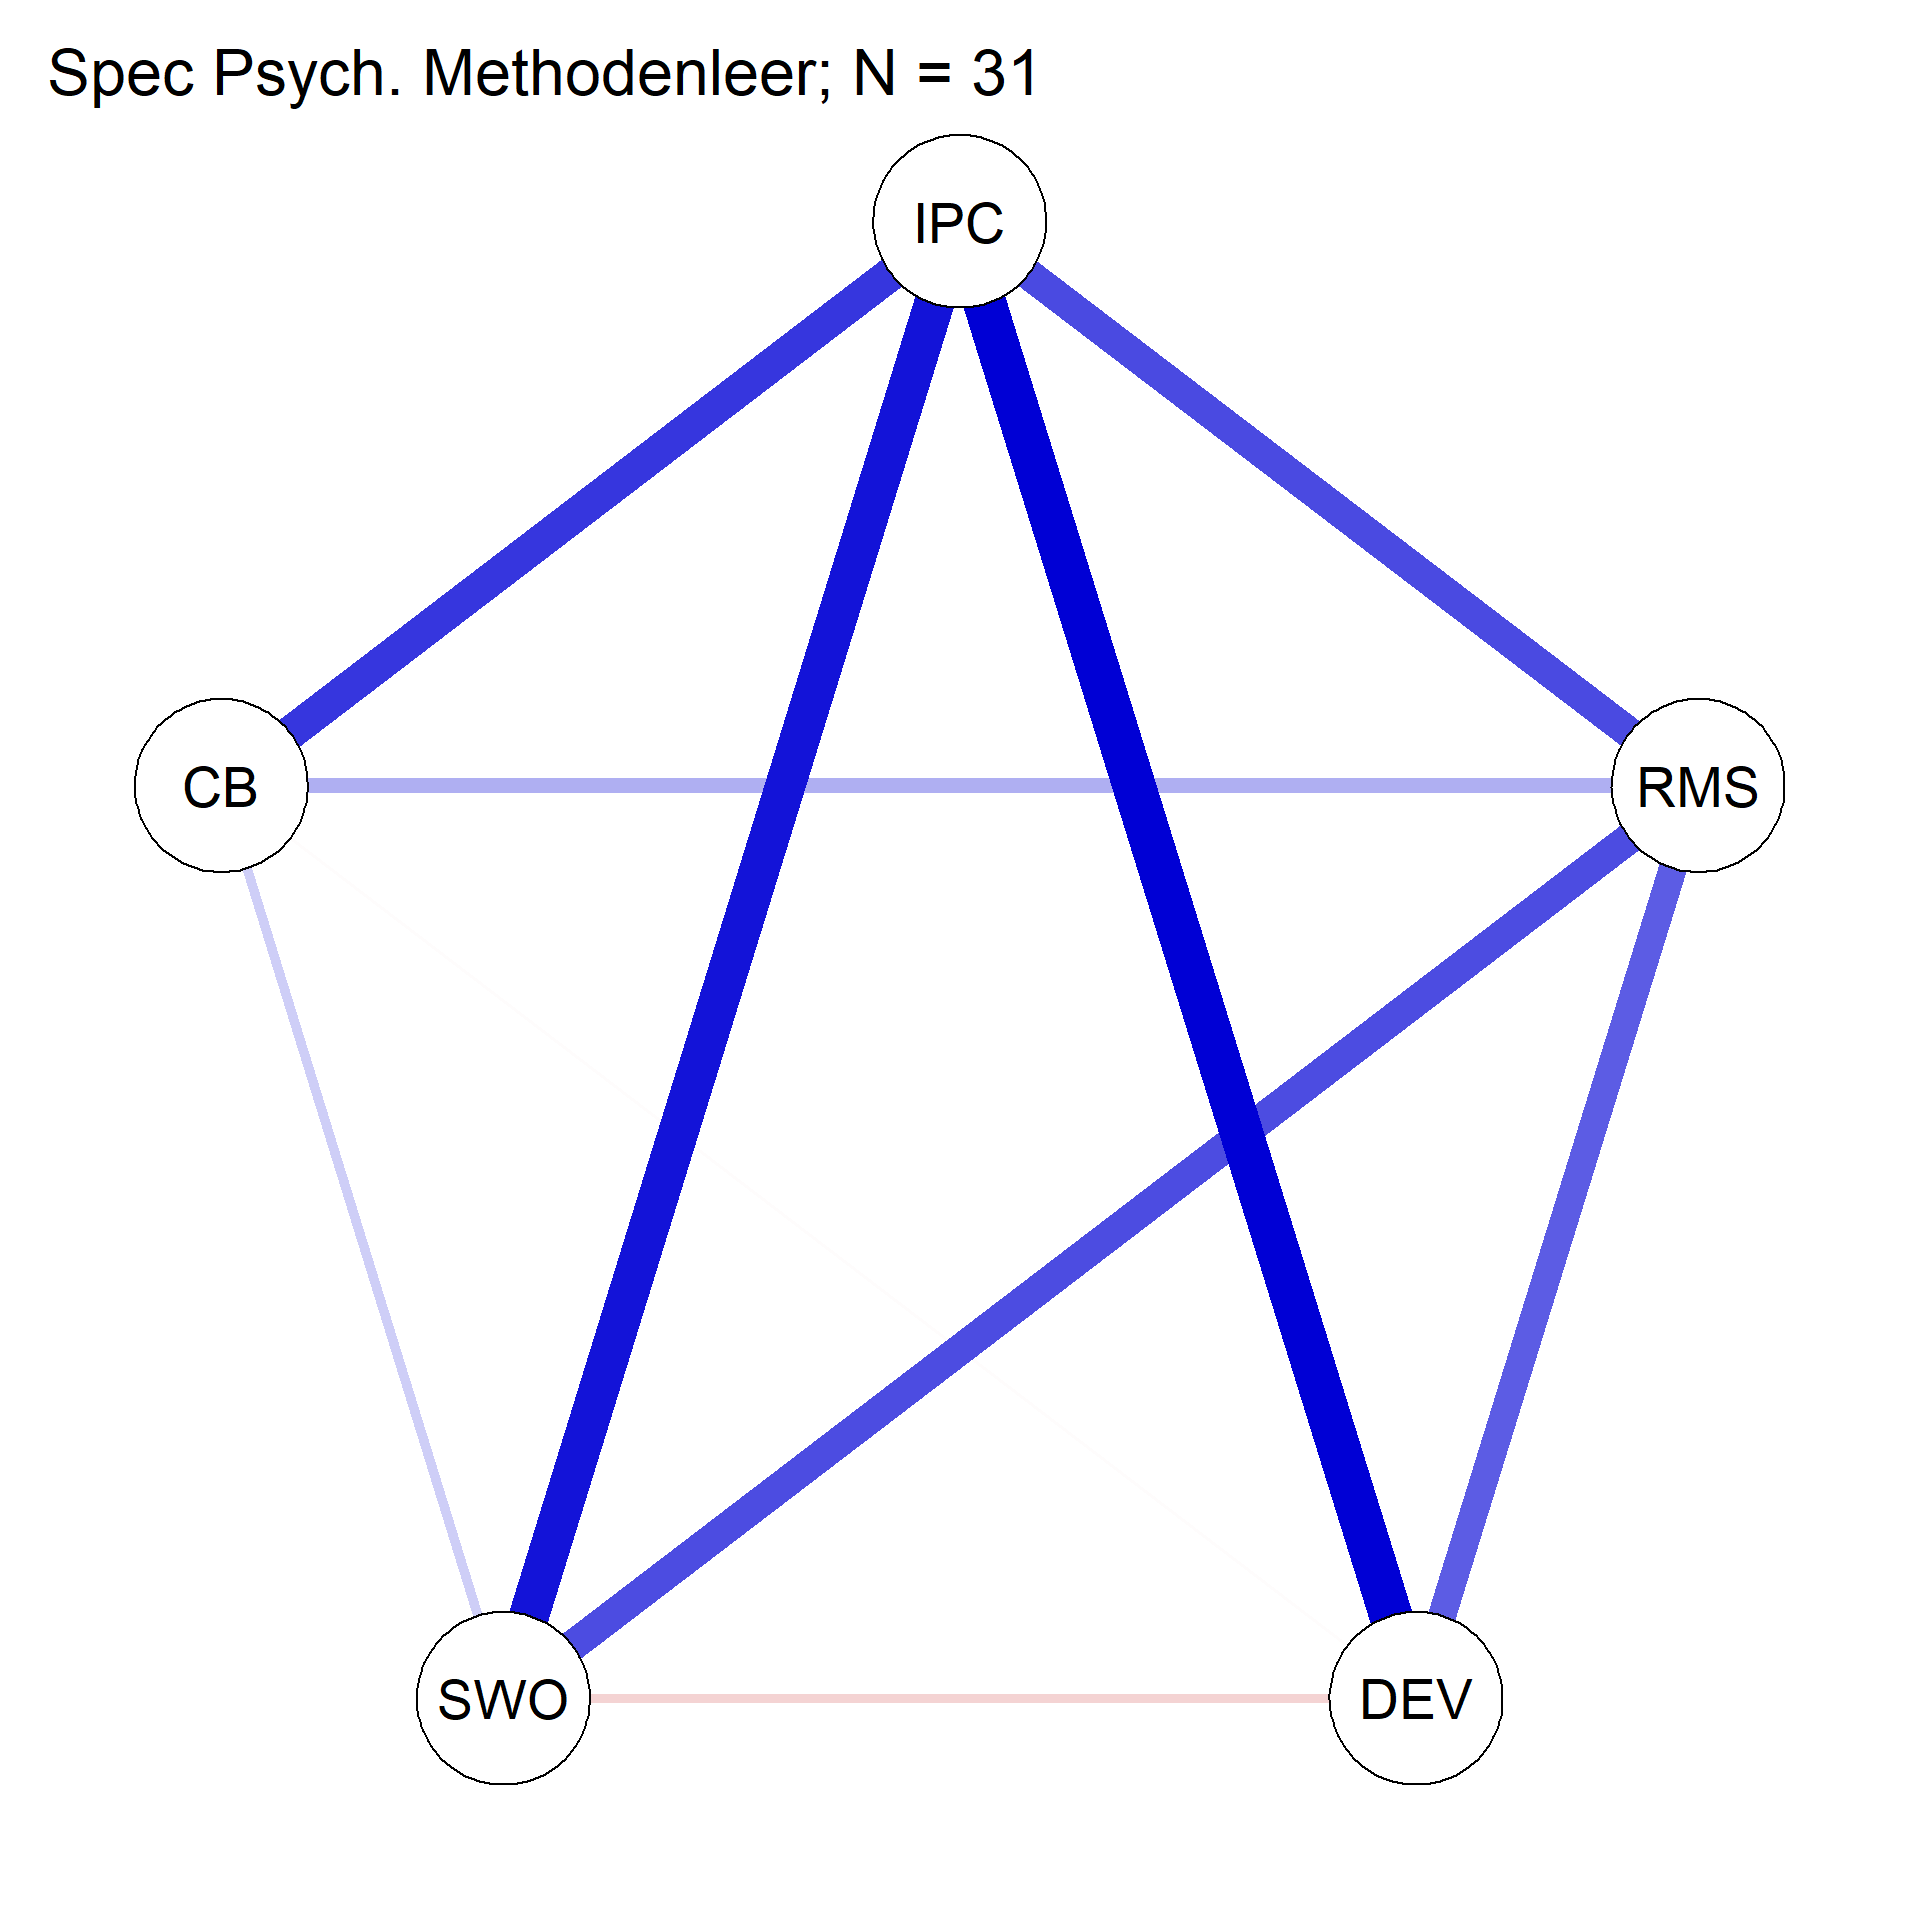
\includegraphics{2021_IDDC_Final-Report_Group-7_files/figure-latex/unnamed-chunk-12-1.pdf}

\hypertarget{social-1}{%
\subparagraph{Social}\label{social-1}}

\begin{Shaded}
\begin{Highlighting}[]
\CommentTok{# Create Dummy Variable for "SOC" Specialization: Yes/No}
\NormalTok{dataSOC <-}\StringTok{ }
\StringTok{  }\NormalTok{data_wide }\OperatorTok
\StringTok{      }\KeywordTok{mutate}\NormalTok{(}\DataTypeTok{SOC =} \KeywordTok{ifelse}\NormalTok{(data_wide}\OperatorTok{$}\NormalTok{Specialization }\OperatorTok{==}\StringTok{ "Spec Sociale Psychologie"}\NormalTok{, }\DecValTok{1}\NormalTok{, }\DecValTok{0}\NormalTok{))}


\NormalTok{networkSOC <-}\StringTok{ }\KeywordTok{estimateNetwork}\NormalTok{(dataSOC[,}\OperatorTok{-}\KeywordTok{c}\NormalTok{(}\DecValTok{1}\OperatorTok{:}\DecValTok{2}\NormalTok{)],}
                               \DataTypeTok{default =} \StringTok{"pcor"}\NormalTok{,}
                               \DataTypeTok{corMethod =} \StringTok{"spearman"}\NormalTok{)}

\KeywordTok{qgraph}\NormalTok{(networkSOC}\OperatorTok{$}\NormalTok{graph,}
       \DataTypeTok{layout =} \StringTok{"circle"}\NormalTok{,}
       \DataTypeTok{theme =} \StringTok{"colorblind"}\NormalTok{,}
       \DataTypeTok{title.cex =} \DecValTok{2}\NormalTok{,}
       \DataTypeTok{title =} \KeywordTok{paste}\NormalTok{(}\StringTok{"Spec Sociale Psychologie (Yes/No); N ="}\NormalTok{, }\KeywordTok{nrow}\NormalTok{(dataSOC)))}
\end{Highlighting}
\end{Shaded}

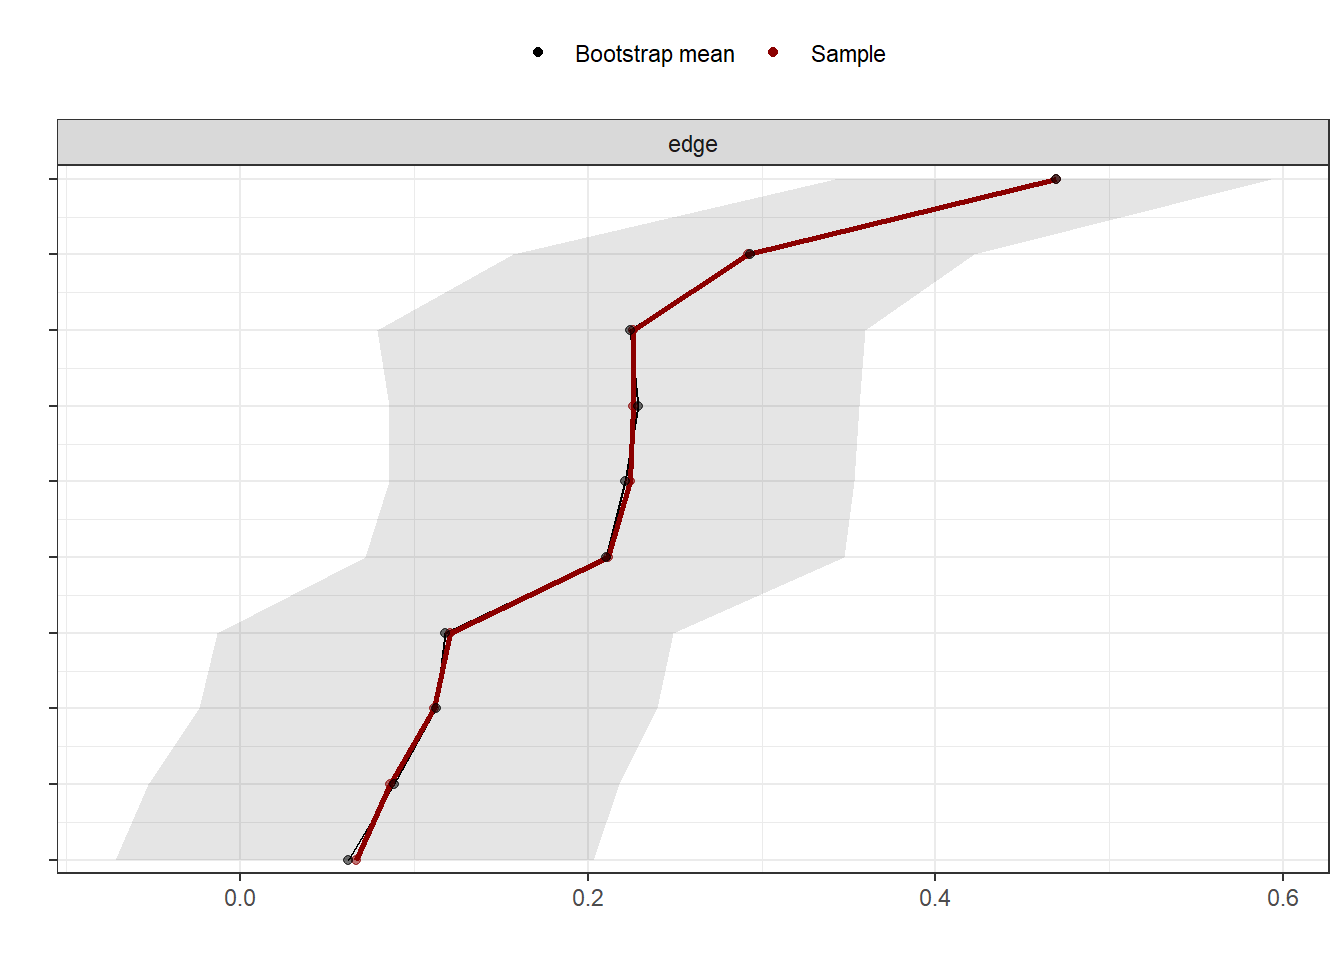
\includegraphics{2021_IDDC_Final-Report_Group-7_files/figure-latex/unnamed-chunk-13-1.pdf}

\hypertarget{brain-cognition-1}{%
\subparagraph{Brain \& Cognition}\label{brain-cognition-1}}

\begin{Shaded}
\begin{Highlighting}[]
\CommentTok{# Create Dummy Variable for "BC" Specialization: Yes/No}
\NormalTok{dataBC <-}\StringTok{ }
\StringTok{  }\NormalTok{data_wide }\OperatorTok
\StringTok{      }\KeywordTok{mutate}\NormalTok{(}\DataTypeTok{BC =} \KeywordTok{ifelse}\NormalTok{(data_wide}\OperatorTok{$}\NormalTok{Specialization }\OperatorTok{==}\StringTok{ "Spec Brein en Cognitie"}\NormalTok{, }\DecValTok{1}\NormalTok{, }\DecValTok{0}\NormalTok{))}


\NormalTok{networkBC <-}\StringTok{ }\KeywordTok{estimateNetwork}\NormalTok{(dataBC[,}\OperatorTok{-}\KeywordTok{c}\NormalTok{(}\DecValTok{1}\OperatorTok{:}\DecValTok{2}\NormalTok{)],}
                               \DataTypeTok{default =} \StringTok{"pcor"}\NormalTok{,}
                               \DataTypeTok{corMethod =} \StringTok{"spearman"}\NormalTok{)}

\KeywordTok{qgraph}\NormalTok{(networkBC}\OperatorTok{$}\NormalTok{graph,}
       \DataTypeTok{layout =} \StringTok{"circle"}\NormalTok{,}
       \DataTypeTok{theme =} \StringTok{"colorblind"}\NormalTok{,}
       \DataTypeTok{title.cex =} \DecValTok{2}\NormalTok{,}
       \DataTypeTok{title =} \KeywordTok{paste}\NormalTok{(}\StringTok{"Spec Brein en Cognitie (Yes/No); N ="}\NormalTok{, }\KeywordTok{nrow}\NormalTok{(dataBC)))}
\end{Highlighting}
\end{Shaded}

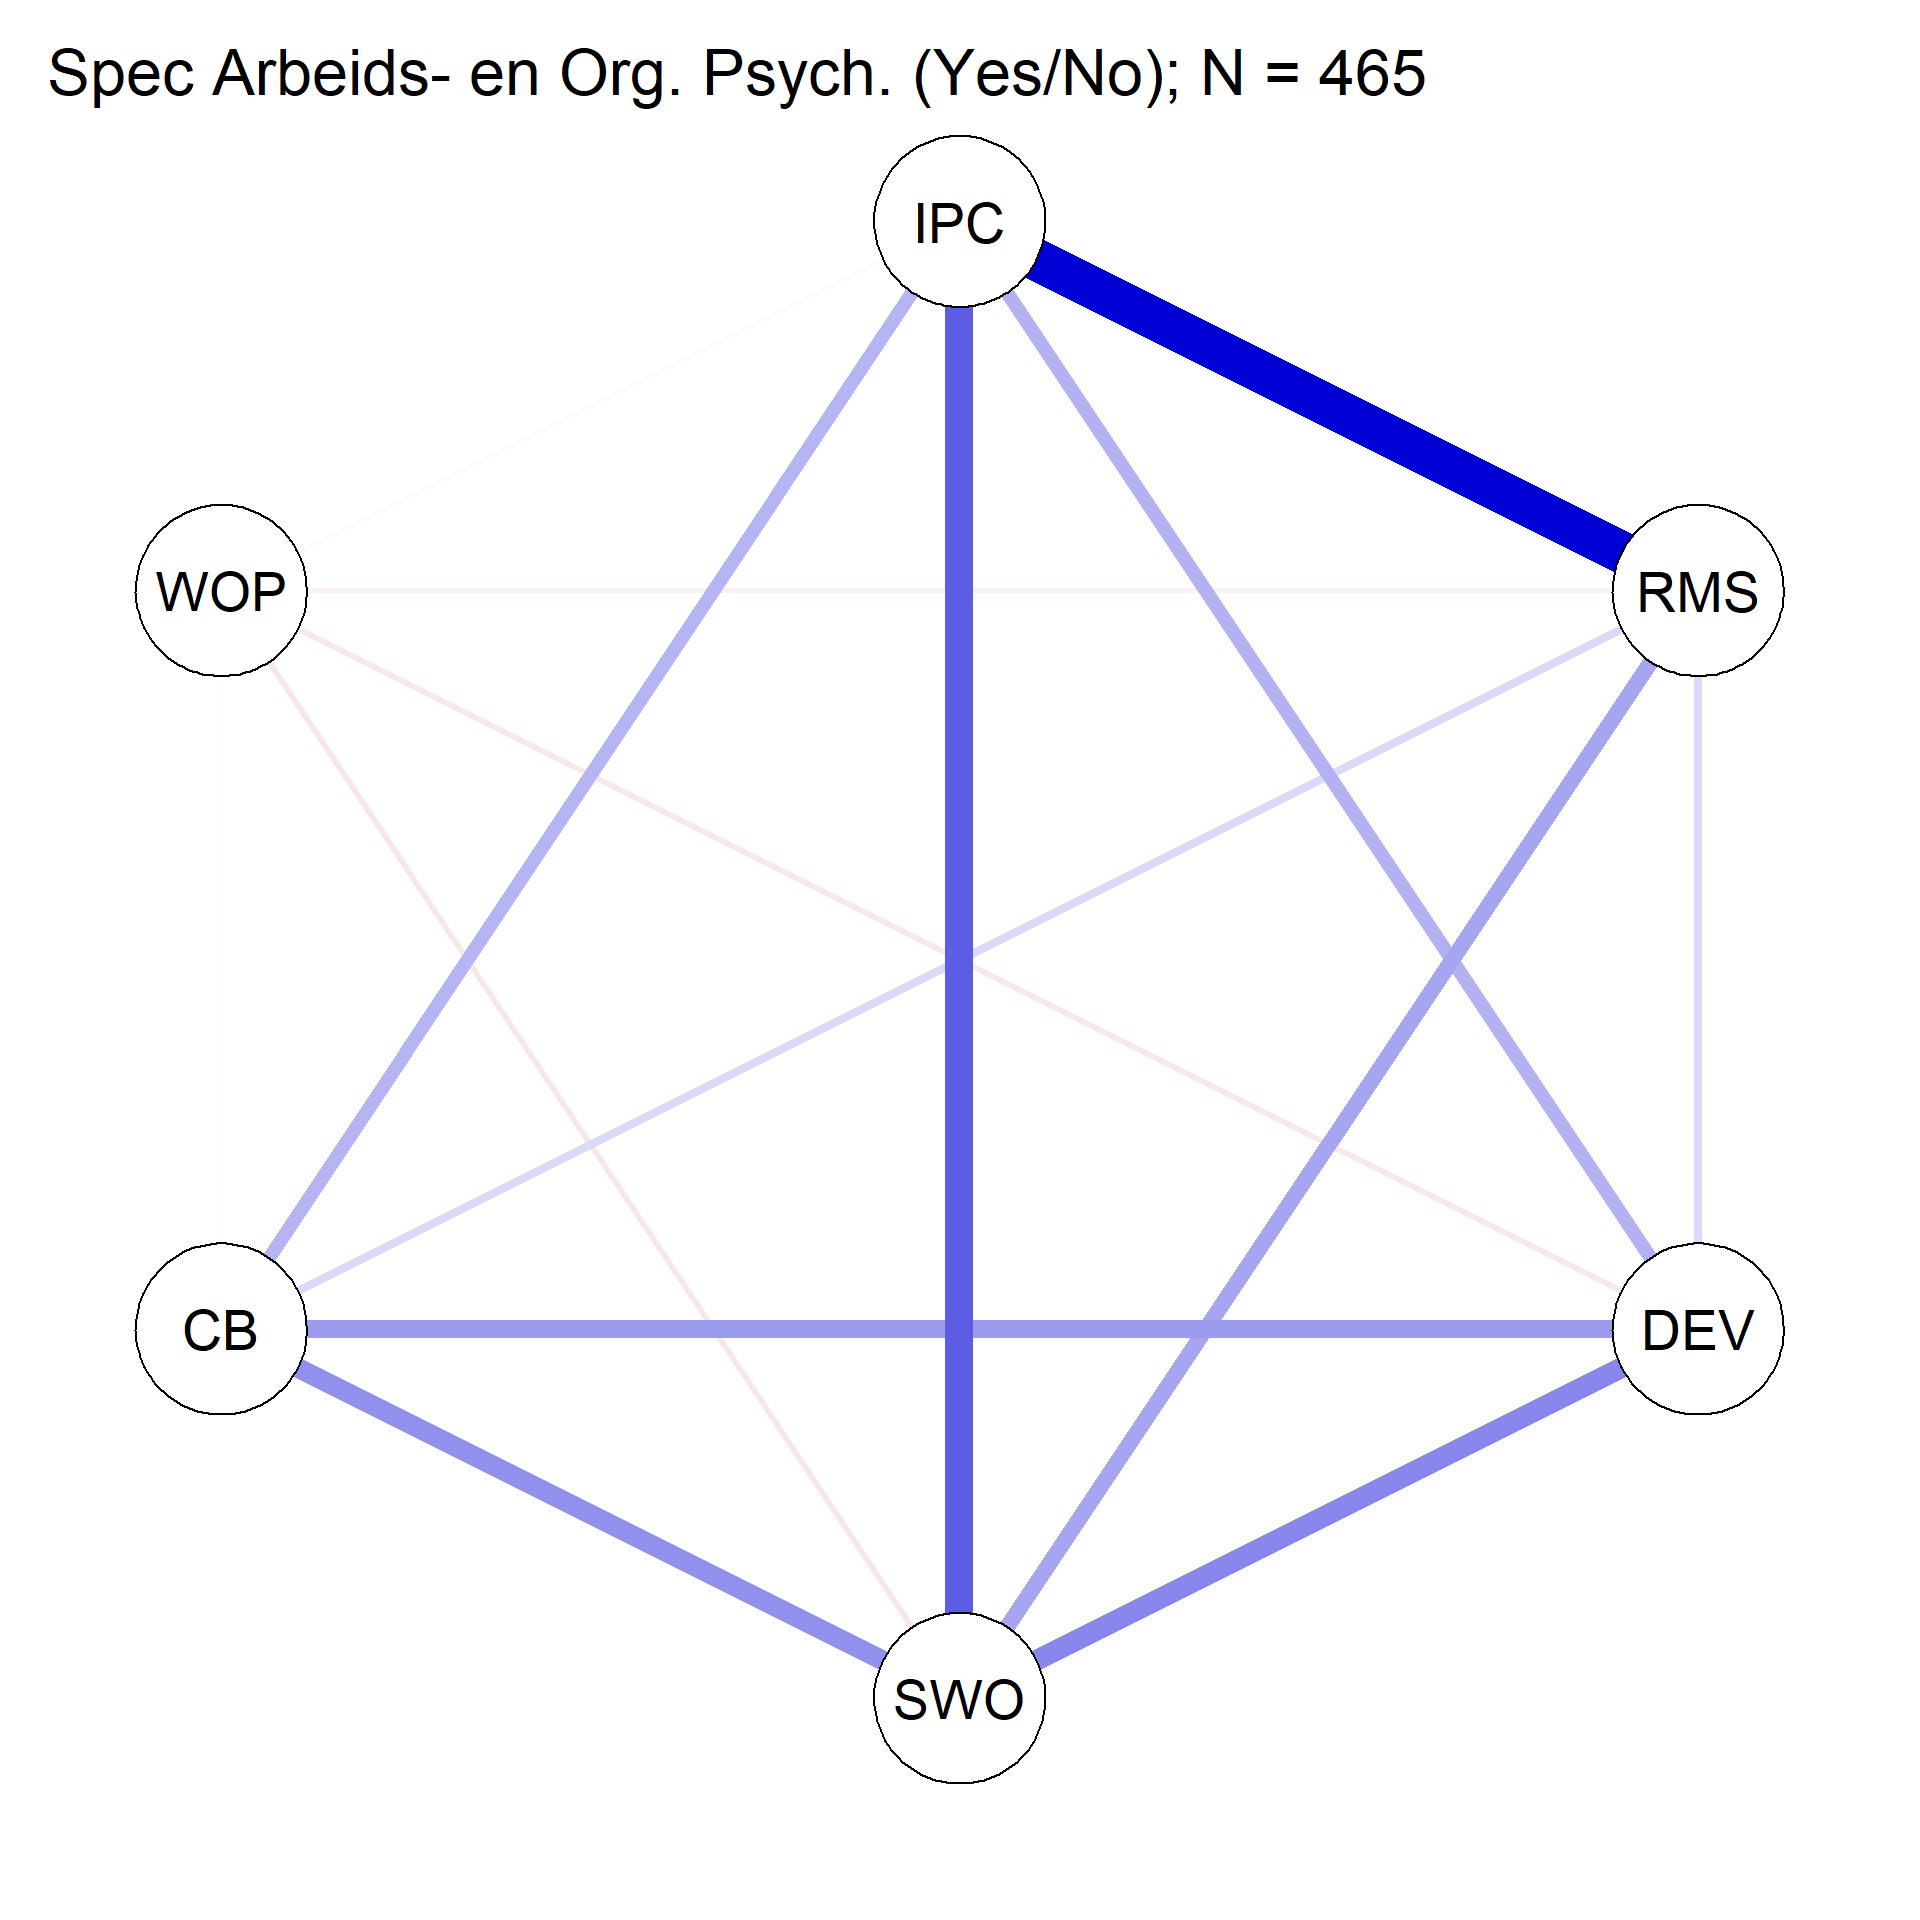
\includegraphics{2021_IDDC_Final-Report_Group-7_files/figure-latex/unnamed-chunk-14-1.pdf}

\hypertarget{clinical-dev-1}{%
\subparagraph{Clinical Dev}\label{clinical-dev-1}}

\begin{Shaded}
\begin{Highlighting}[]
\CommentTok{# Create Dummy Variable for "DEV" Specialization: Yes/No}
\NormalTok{dataDEV <-}\StringTok{ }
\StringTok{  }\NormalTok{data_wide }\OperatorTok
\StringTok{      }\KeywordTok{mutate}\NormalTok{(}\DataTypeTok{CDV =} \KeywordTok{ifelse}\NormalTok{(data_wide}\OperatorTok{$}\NormalTok{Specialization }\OperatorTok{==}\StringTok{ "Spec Klinische Ontwikkelingsps"}\NormalTok{, }\DecValTok{1}\NormalTok{, }\DecValTok{0}\NormalTok{))}


\NormalTok{networkDEV <-}\StringTok{ }\KeywordTok{estimateNetwork}\NormalTok{(dataDEV[,}\OperatorTok{-}\KeywordTok{c}\NormalTok{(}\DecValTok{1}\OperatorTok{:}\DecValTok{2}\NormalTok{)],}
                               \DataTypeTok{default =} \StringTok{"pcor"}\NormalTok{,}
                               \DataTypeTok{corMethod =} \StringTok{"spearman"}\NormalTok{)}

\KeywordTok{qgraph}\NormalTok{(networkDEV}\OperatorTok{$}\NormalTok{graph,}
       \DataTypeTok{layout =} \StringTok{"circle"}\NormalTok{,}
       \DataTypeTok{theme =} \StringTok{"colorblind"}\NormalTok{,}
       \DataTypeTok{title.cex =} \DecValTok{2}\NormalTok{,}
       \DataTypeTok{title =} \KeywordTok{paste}\NormalTok{(}\StringTok{"Spec Klinische Ontwikkelingsps(Yes/No); N ="}\NormalTok{, }\KeywordTok{nrow}\NormalTok{(dataDEV)))}
\end{Highlighting}
\end{Shaded}

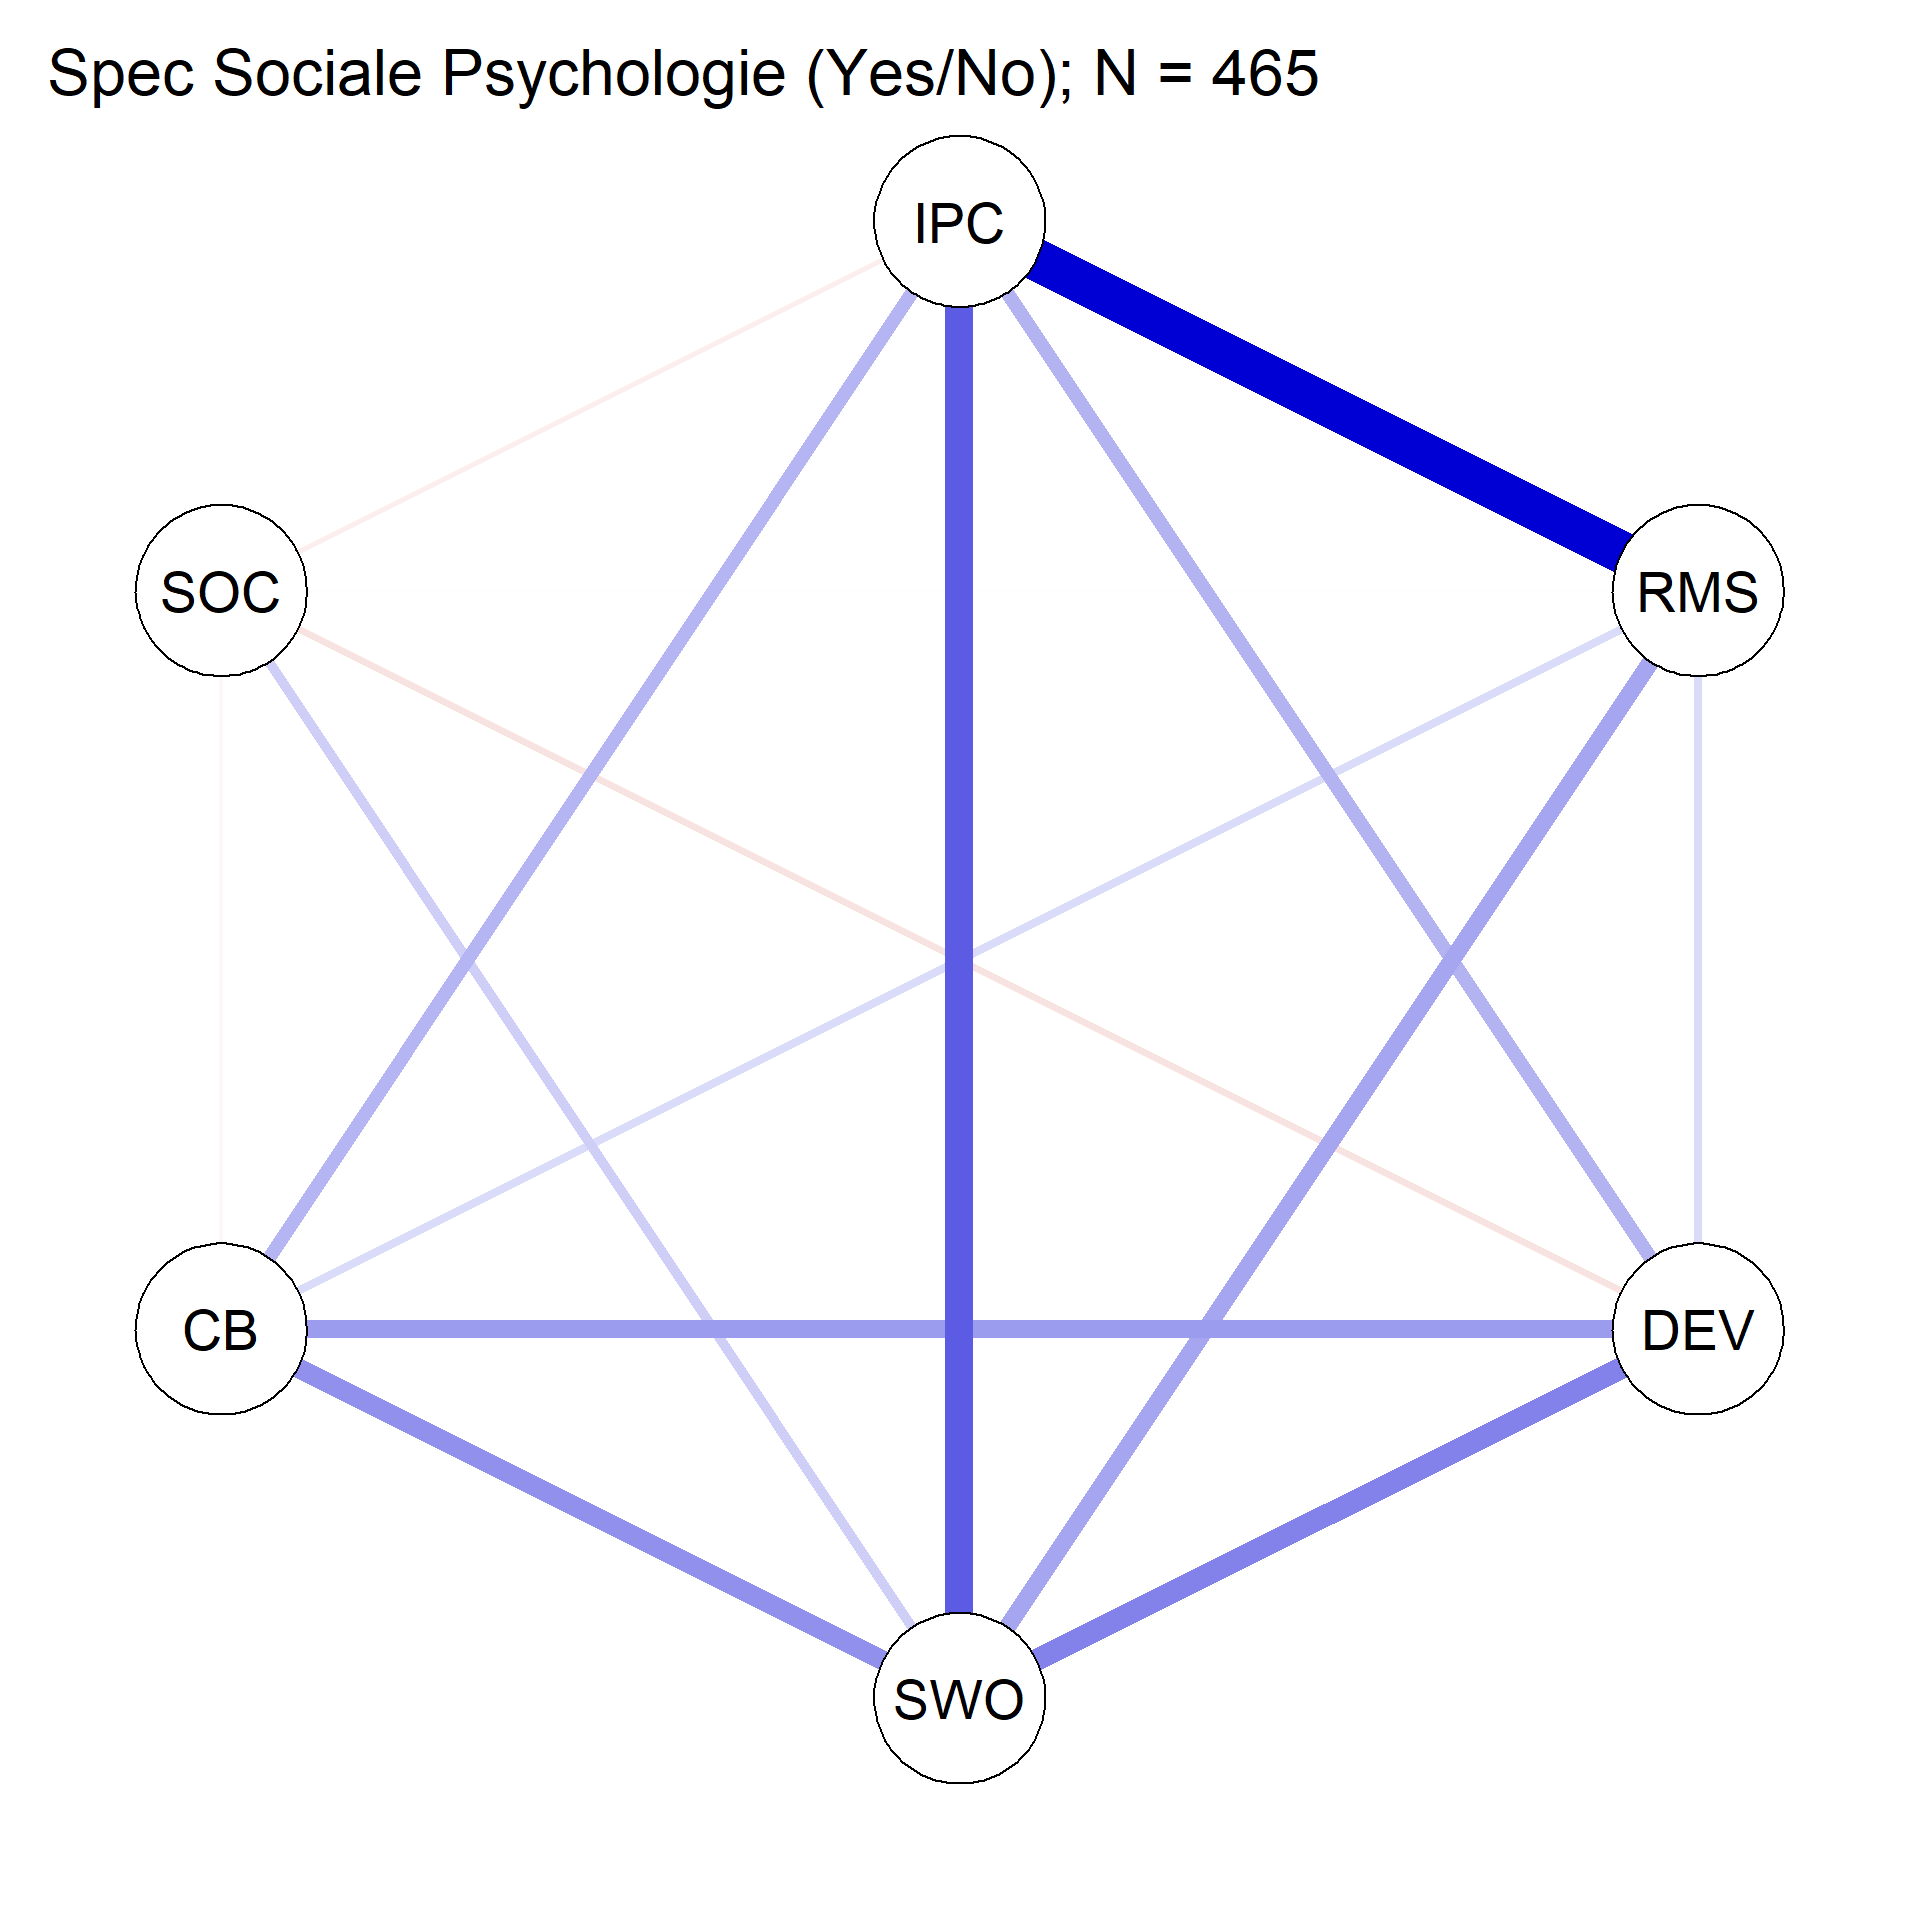
\includegraphics{2021_IDDC_Final-Report_Group-7_files/figure-latex/unnamed-chunk-15-1.pdf}

\hypertarget{clinical-neuro-1}{%
\subparagraph{Clinical Neuro}\label{clinical-neuro-1}}

\begin{Shaded}
\begin{Highlighting}[]
\CommentTok{# Create Dummy Variable for "DEV" Specialization: Yes/No}
\NormalTok{dataCNP <-}\StringTok{ }
\StringTok{  }\NormalTok{data_wide }\OperatorTok
\StringTok{      }\KeywordTok{mutate}\NormalTok{(}\DataTypeTok{CNP =} \KeywordTok{ifelse}\NormalTok{(data_wide}\OperatorTok{$}\NormalTok{Specialization }\OperatorTok{==}\StringTok{ "Spec Klinische Neuropsych."}\NormalTok{, }\DecValTok{1}\NormalTok{, }\DecValTok{0}\NormalTok{))}


\NormalTok{networkCNP <-}\StringTok{ }\KeywordTok{estimateNetwork}\NormalTok{(dataCNP[,}\OperatorTok{-}\KeywordTok{c}\NormalTok{(}\DecValTok{1}\OperatorTok{:}\DecValTok{2}\NormalTok{)],}
                               \DataTypeTok{default =} \StringTok{"pcor"}\NormalTok{,}
                               \DataTypeTok{corMethod =} \StringTok{"spearman"}\NormalTok{)}

\KeywordTok{qgraph}\NormalTok{(networkCNP}\OperatorTok{$}\NormalTok{graph,}
       \DataTypeTok{layout =} \StringTok{"circle"}\NormalTok{,}
       \DataTypeTok{theme =} \StringTok{"colorblind"}\NormalTok{,}
       \DataTypeTok{title.cex =} \DecValTok{2}\NormalTok{,}
       \DataTypeTok{title =} \KeywordTok{paste}\NormalTok{(}\StringTok{"Spec Klinische Neuropsych.(Yes/No); N ="}\NormalTok{, }\KeywordTok{nrow}\NormalTok{(dataCNP)))}
\end{Highlighting}
\end{Shaded}

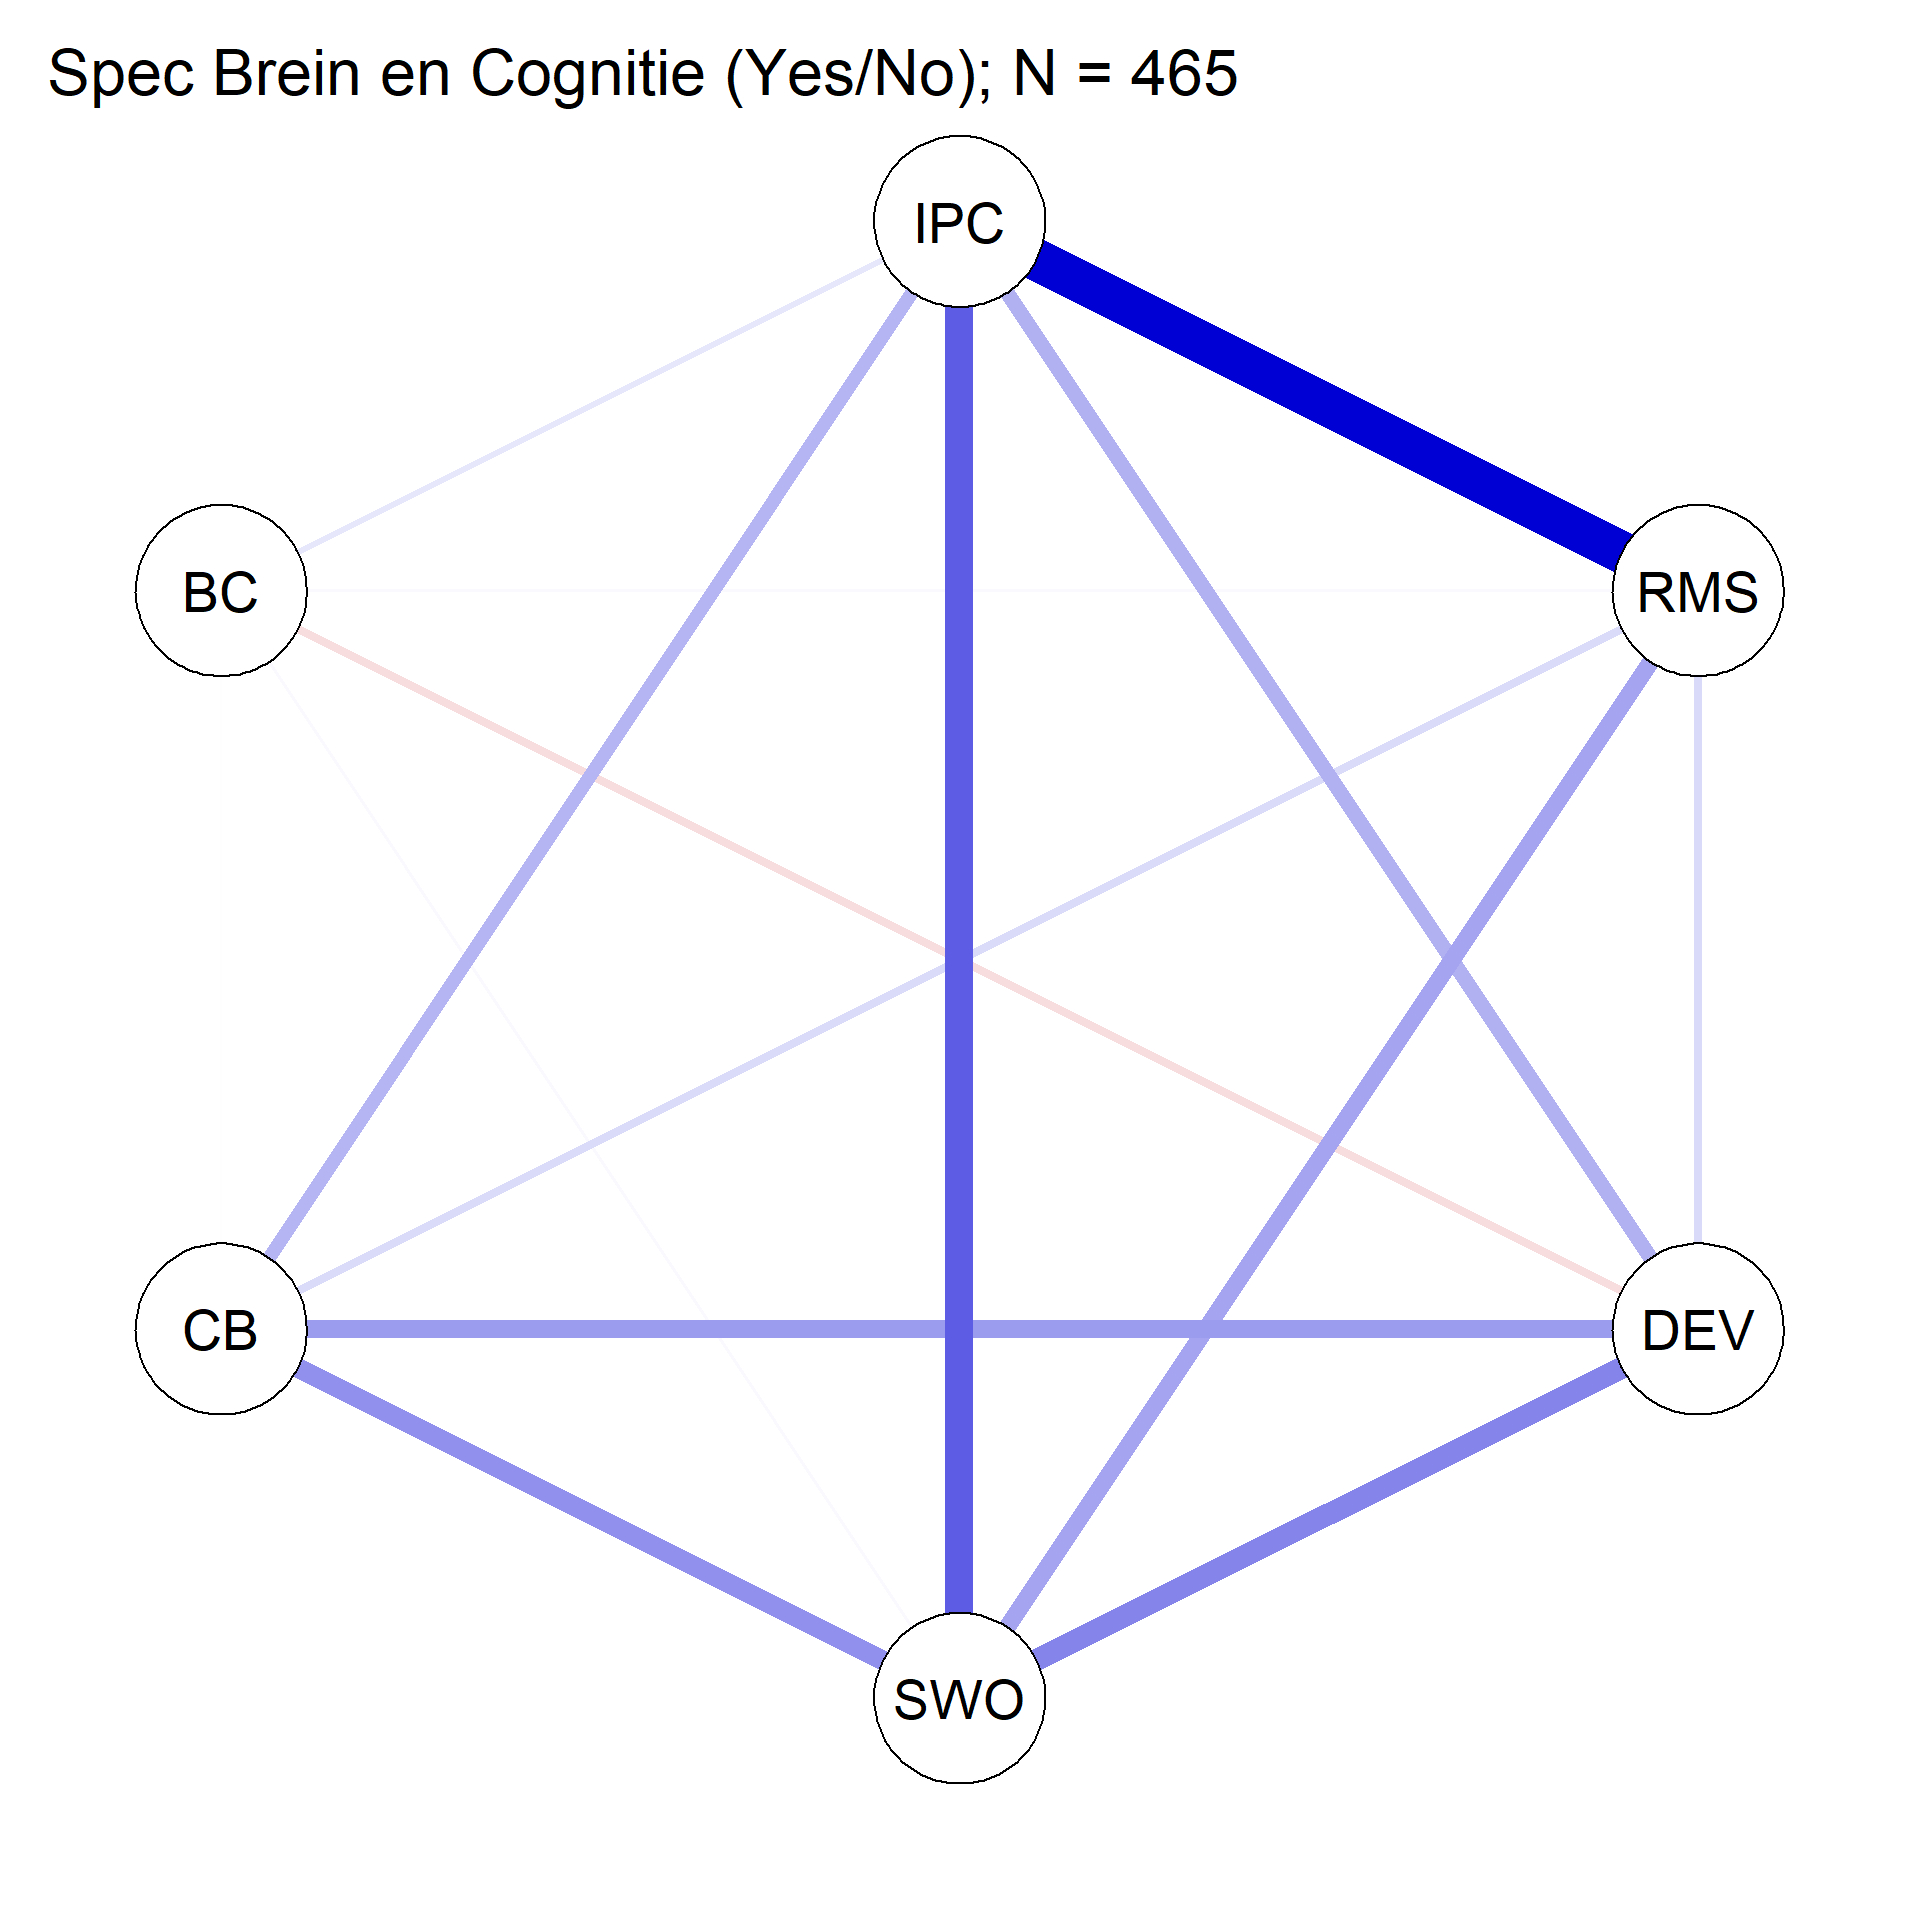
\includegraphics{2021_IDDC_Final-Report_Group-7_files/figure-latex/unnamed-chunk-16-1.pdf}

\hypertarget{methods-1}{%
\subparagraph{Methods}\label{methods-1}}

\begin{Shaded}
\begin{Highlighting}[]
\CommentTok{# Create Dummy Variable for "PML" Specialization: Yes/No}
\NormalTok{dataPML <-}\StringTok{ }
\StringTok{  }\NormalTok{data_wide }\OperatorTok
\StringTok{      }\KeywordTok{mutate}\NormalTok{(}\DataTypeTok{PML =} \KeywordTok{ifelse}\NormalTok{(data_wide}\OperatorTok{$}\NormalTok{Specialization }\OperatorTok{==}\StringTok{ "Spec Psych. Methodenleer"}\NormalTok{, }\DecValTok{1}\NormalTok{, }\DecValTok{0}\NormalTok{))}


\NormalTok{networkPML <-}\StringTok{ }\KeywordTok{estimateNetwork}\NormalTok{(dataPML[,}\OperatorTok{-}\KeywordTok{c}\NormalTok{(}\DecValTok{1}\OperatorTok{:}\DecValTok{2}\NormalTok{)],}
                               \DataTypeTok{default =} \StringTok{"pcor"}\NormalTok{,}
                               \DataTypeTok{corMethod =} \StringTok{"spearman"}\NormalTok{)}

\KeywordTok{qgraph}\NormalTok{(networkPML}\OperatorTok{$}\NormalTok{graph,}
       \DataTypeTok{layout =} \StringTok{"circle"}\NormalTok{,}
       \DataTypeTok{theme =} \StringTok{"colorblind"}\NormalTok{,}
       \DataTypeTok{title.cex =} \DecValTok{2}\NormalTok{,}
       \DataTypeTok{title =} \KeywordTok{paste}\NormalTok{(}\StringTok{"Spec Psych. Methodenleer (Yes/No); N ="}\NormalTok{, }\KeywordTok{nrow}\NormalTok{(dataPML)))}
\end{Highlighting}
\end{Shaded}

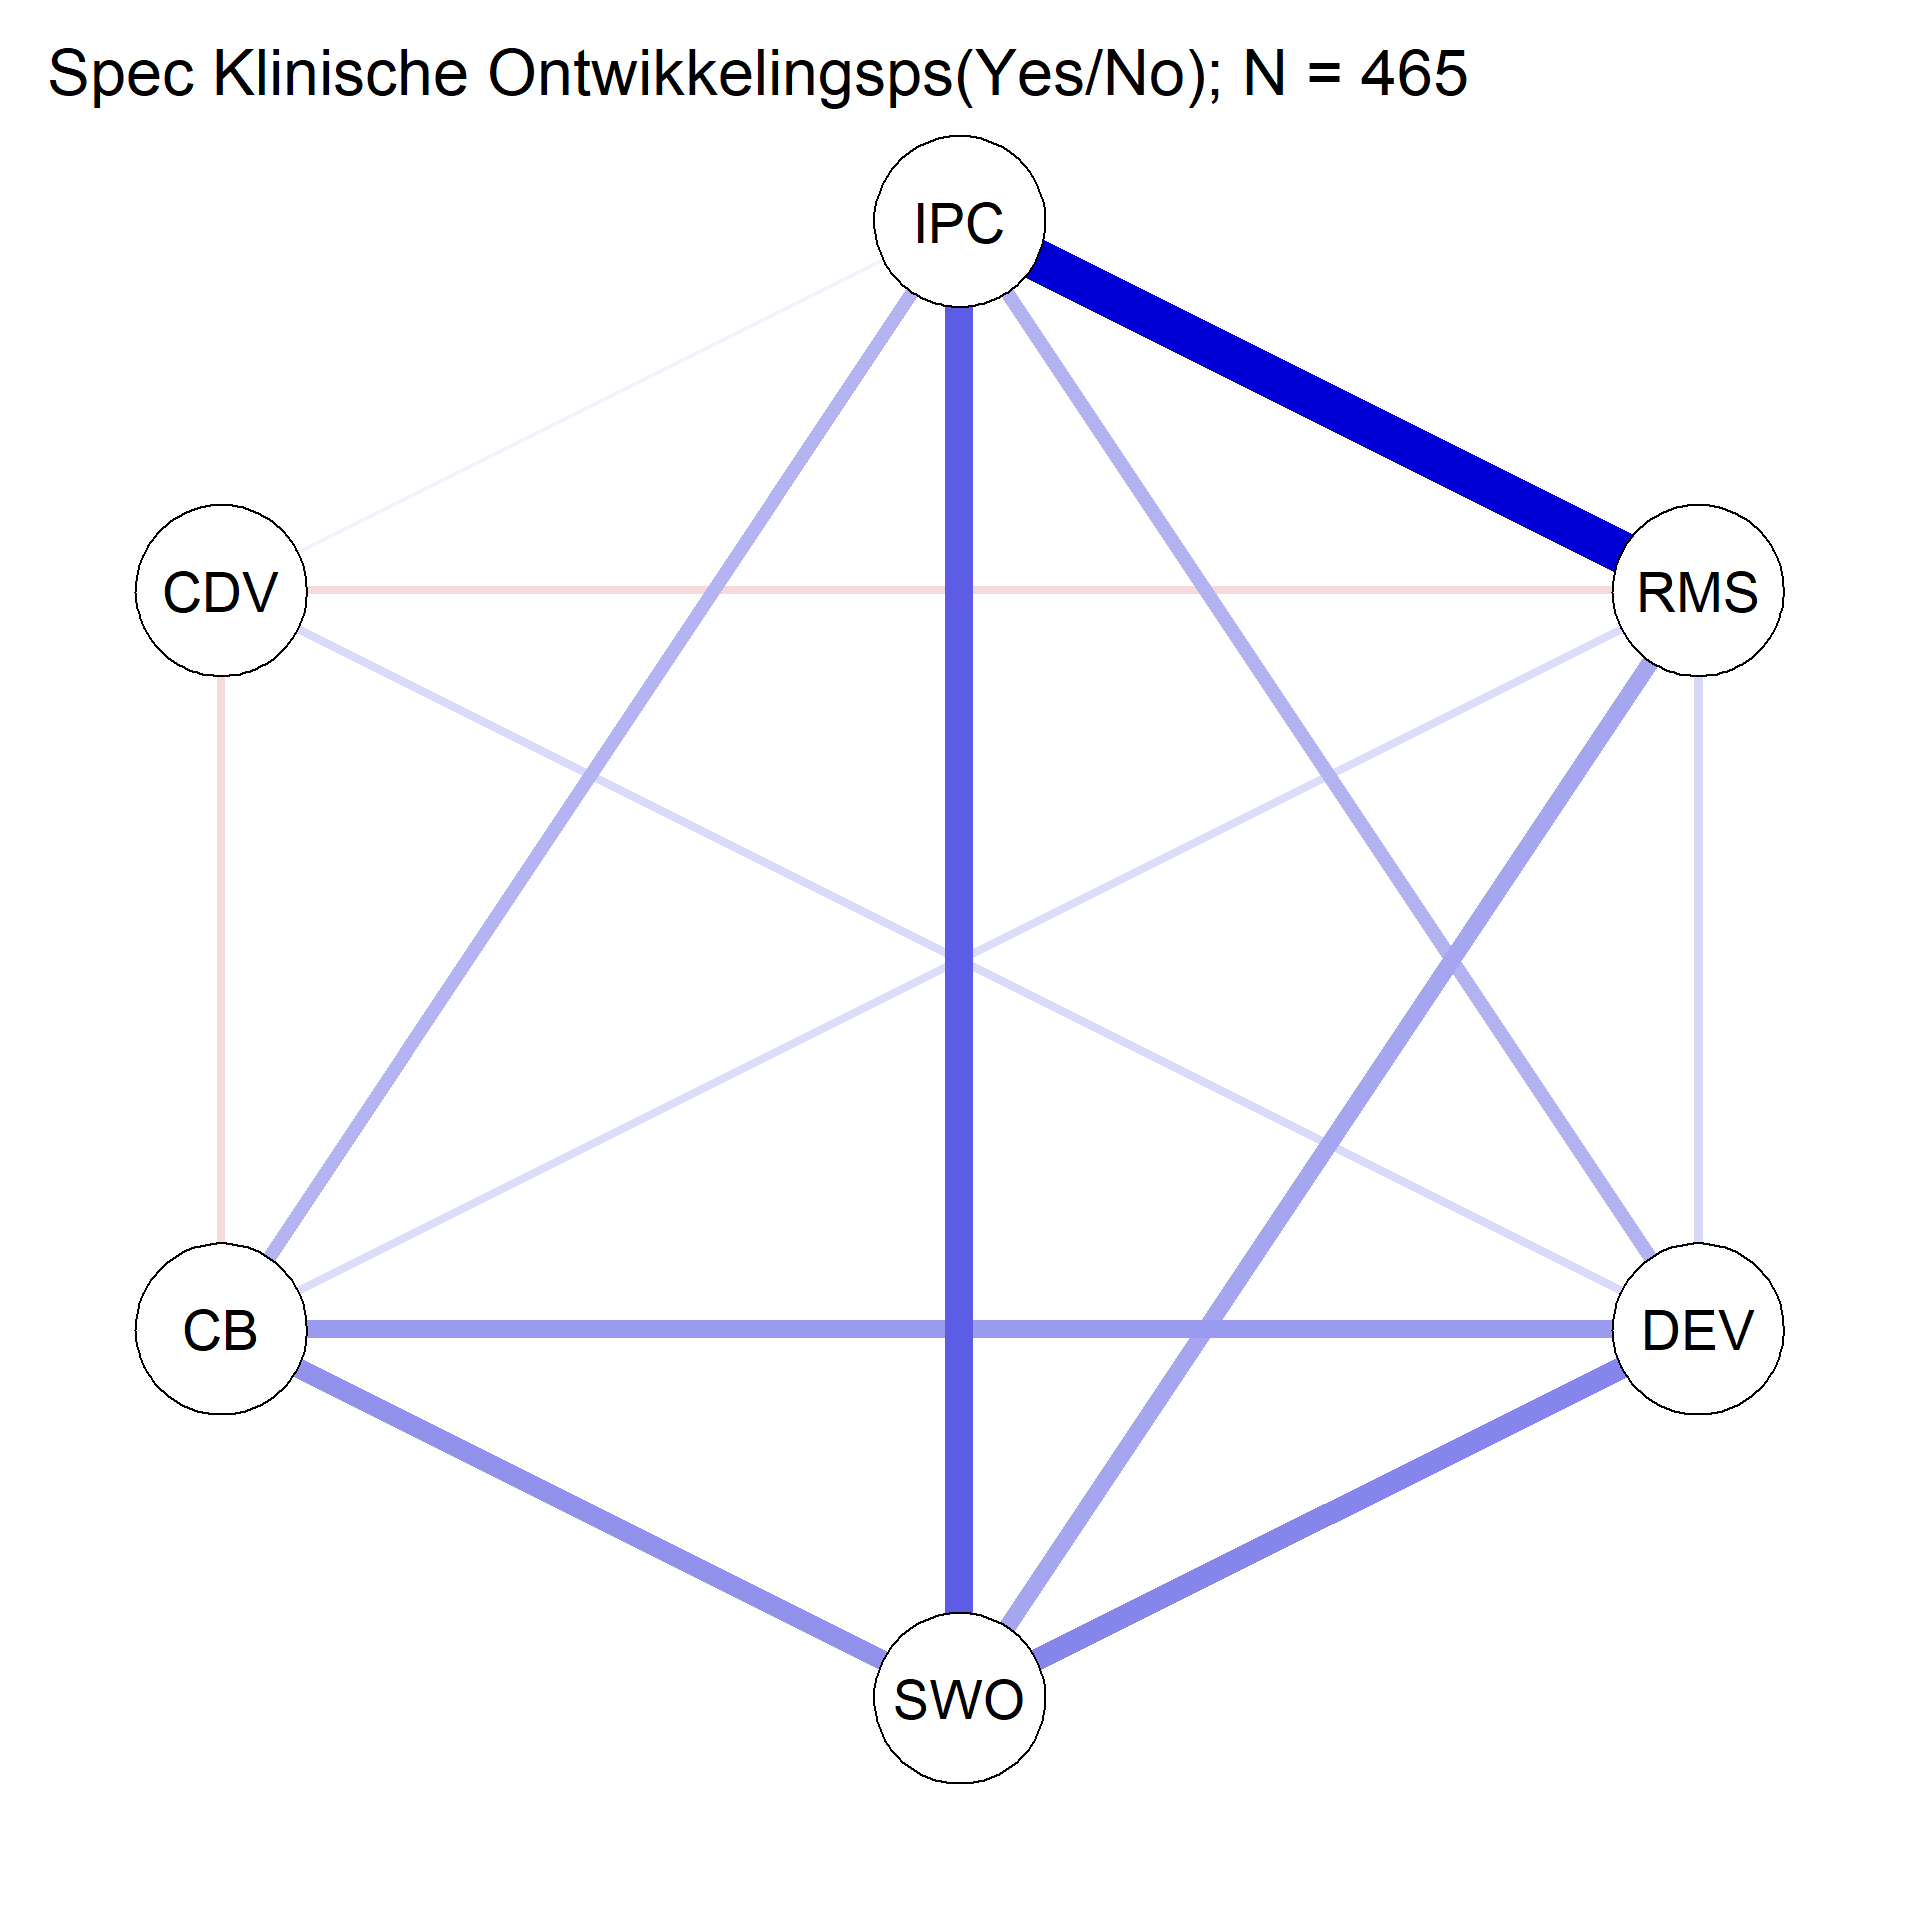
\includegraphics{2021_IDDC_Final-Report_Group-7_files/figure-latex/unnamed-chunk-17-1.pdf}

\hypertarget{centrality-and-stability}{%
\subsection{Centrality and Stability}\label{centrality-and-stability}}

Centrality refers to the relative importance a variable has within the
network. This relative importance derives from either the importance one
variable has on the rest of the network, or from the way the variables
within a network relate.

\hypertarget{overall-network-1}{%
\subsubsection{Overall Network}\label{overall-network-1}}

\hypertarget{stability-checks-for-overall-network}{%
\subparagraph{Stability Checks for Overall
Network}\label{stability-checks-for-overall-network}}

\begin{Shaded}
\begin{Highlighting}[]
\CommentTok{# Estimate a network of all specializations together}
\NormalTok{network <-}\StringTok{ }\KeywordTok{estimateNetwork}\NormalTok{(data_wide[,}\OperatorTok{-}\KeywordTok{c}\NormalTok{(}\DecValTok{1}\OperatorTok{:}\DecValTok{2}\NormalTok{)],}
                           \DataTypeTok{default =} \StringTok{"pcor"}\NormalTok{,}
                           \DataTypeTok{corMethod =} \StringTok{"spearman"}\NormalTok{)}

\CommentTok{# Plot the estimated network}
\KeywordTok{qgraph}\NormalTok{(network}\OperatorTok{$}\NormalTok{graph,}
       \DataTypeTok{layout =} \StringTok{"circle"}\NormalTok{,}
       \DataTypeTok{theme =} \StringTok{"colorblind"}\NormalTok{)}
\end{Highlighting}
\end{Shaded}

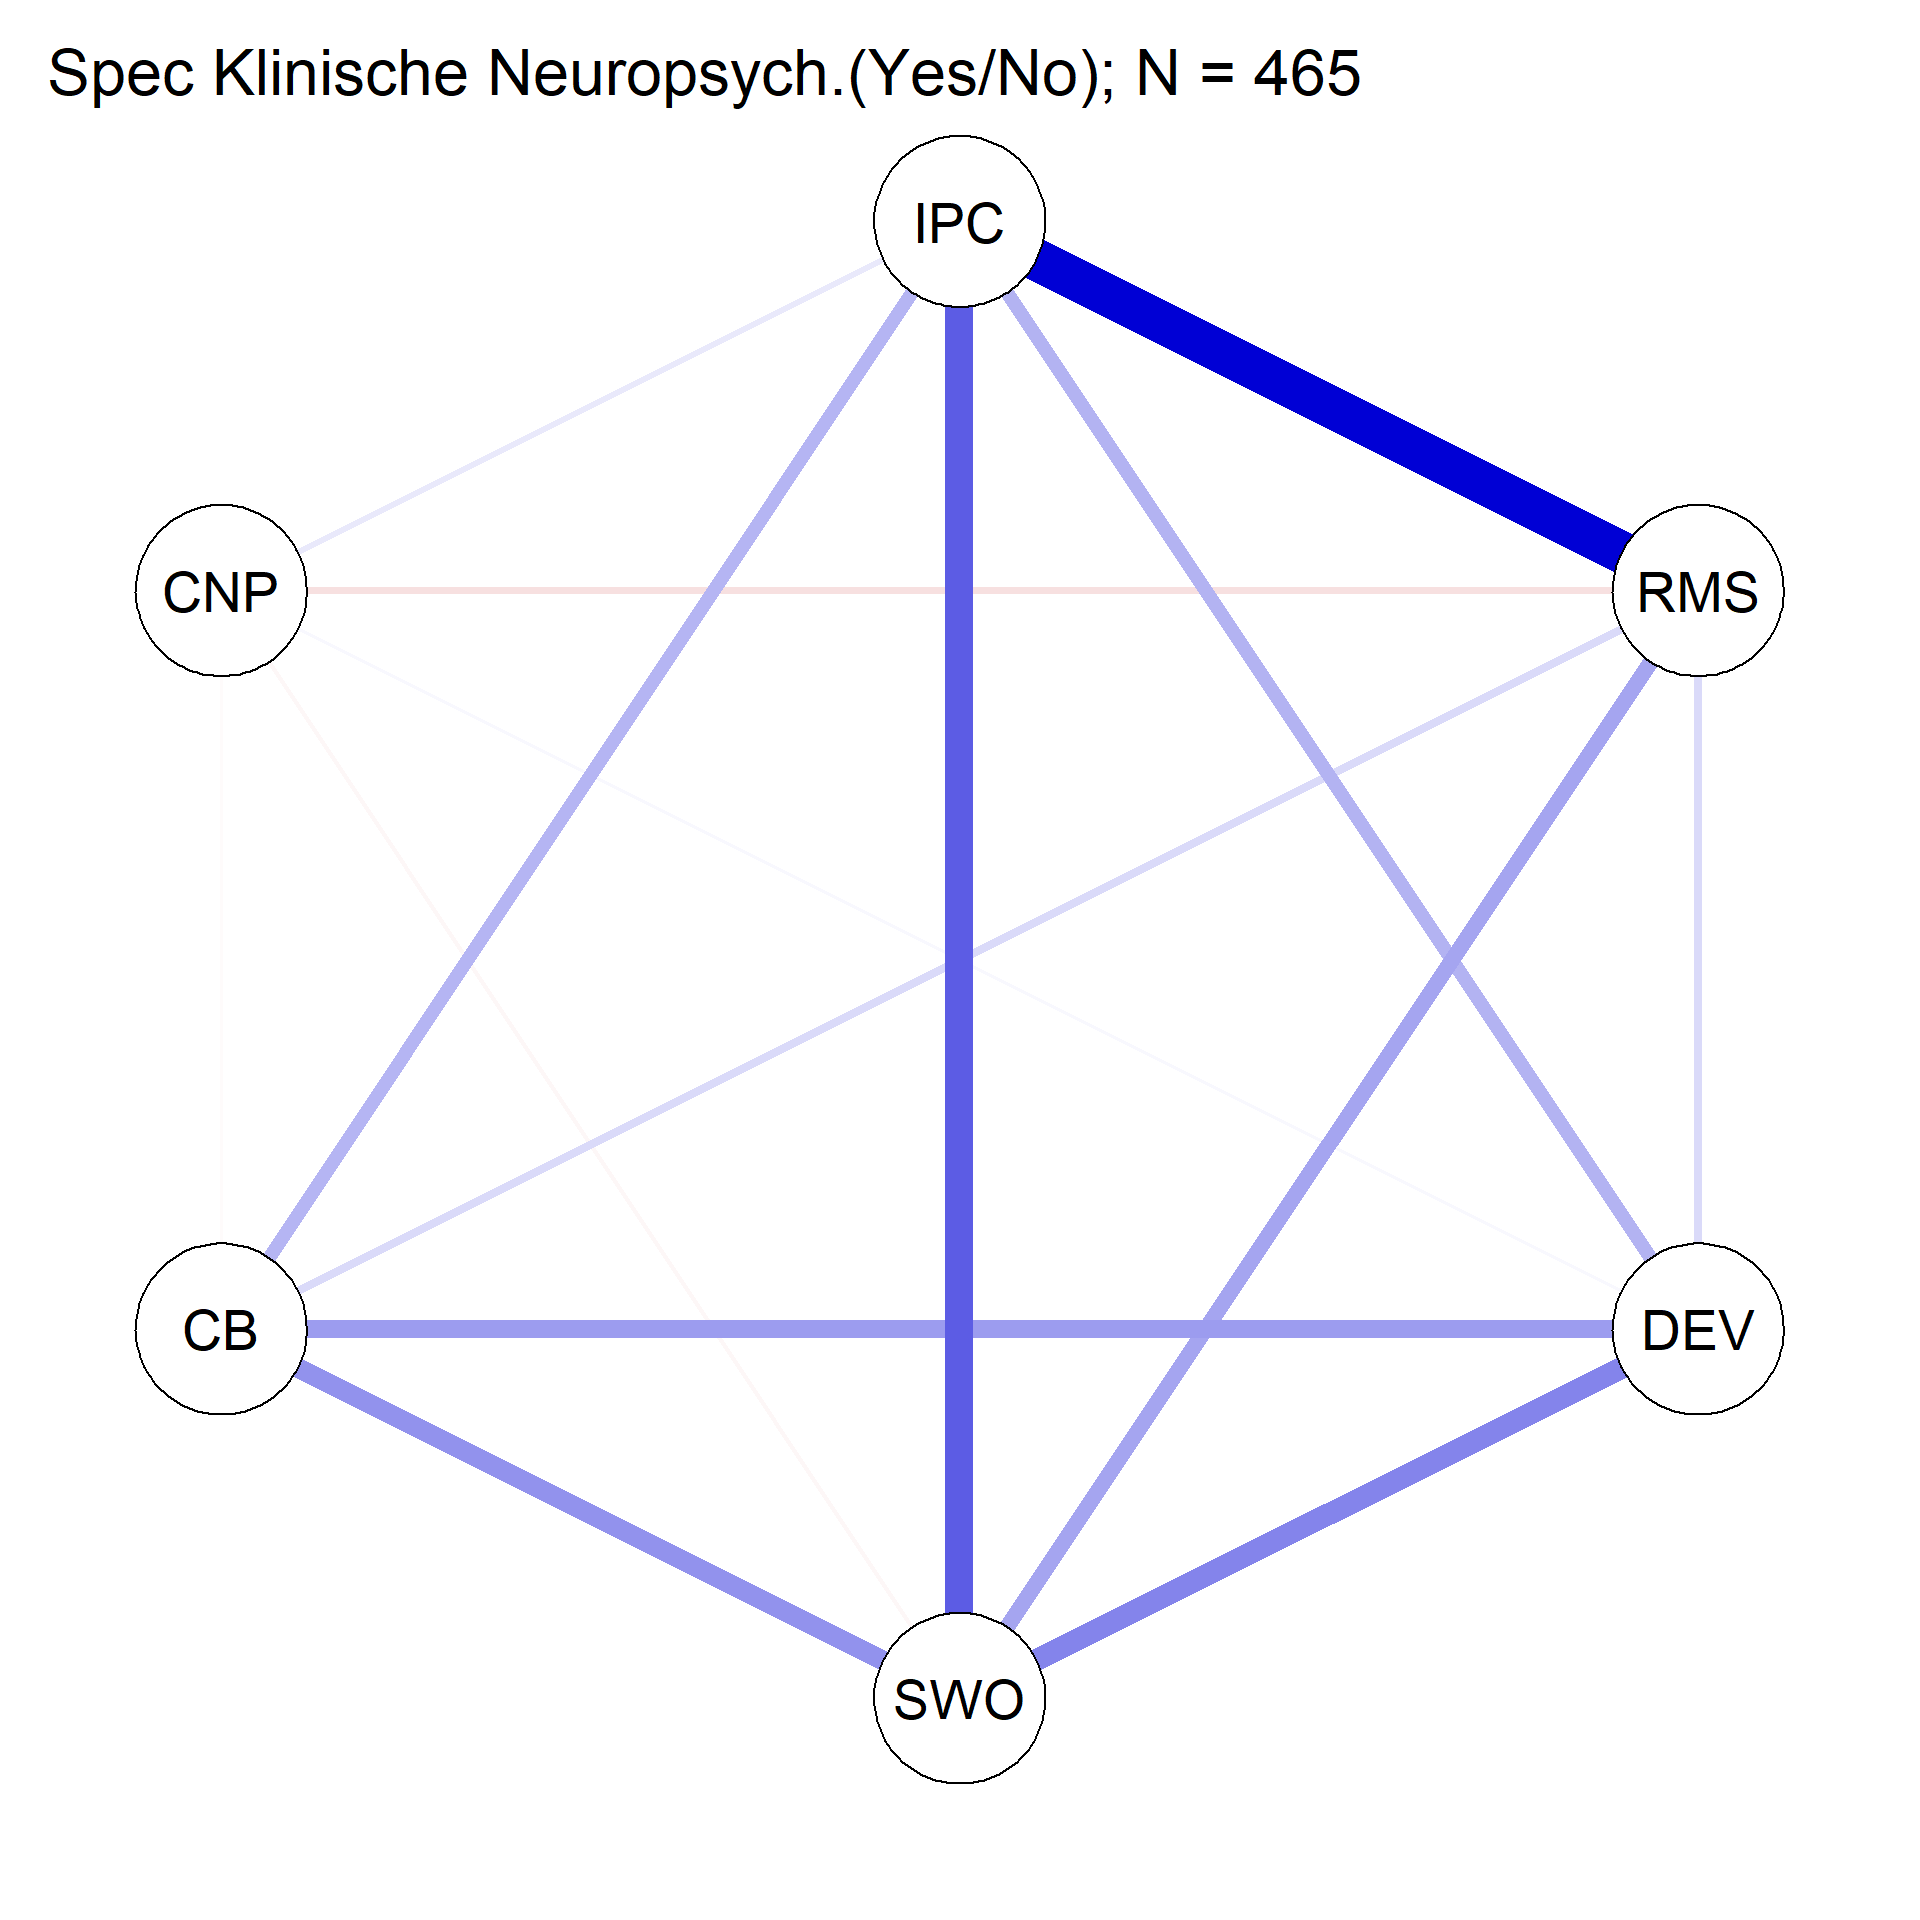
\includegraphics{2021_IDDC_Final-Report_Group-7_files/figure-latex/unnamed-chunk-18-1.pdf}

\begin{Shaded}
\begin{Highlighting}[]
\CommentTok{# Plot the centrality estimates}
\KeywordTok{centralityPlot}\NormalTok{(network}\OperatorTok{$}\NormalTok{graph,}
               \DataTypeTok{include =} \KeywordTok{c}\NormalTok{(}\StringTok{"Strength"}\NormalTok{,}
                           \StringTok{"Closeness"}\NormalTok{,}
                           \StringTok{"Betweenness"}\NormalTok{))}
\end{Highlighting}
\end{Shaded}

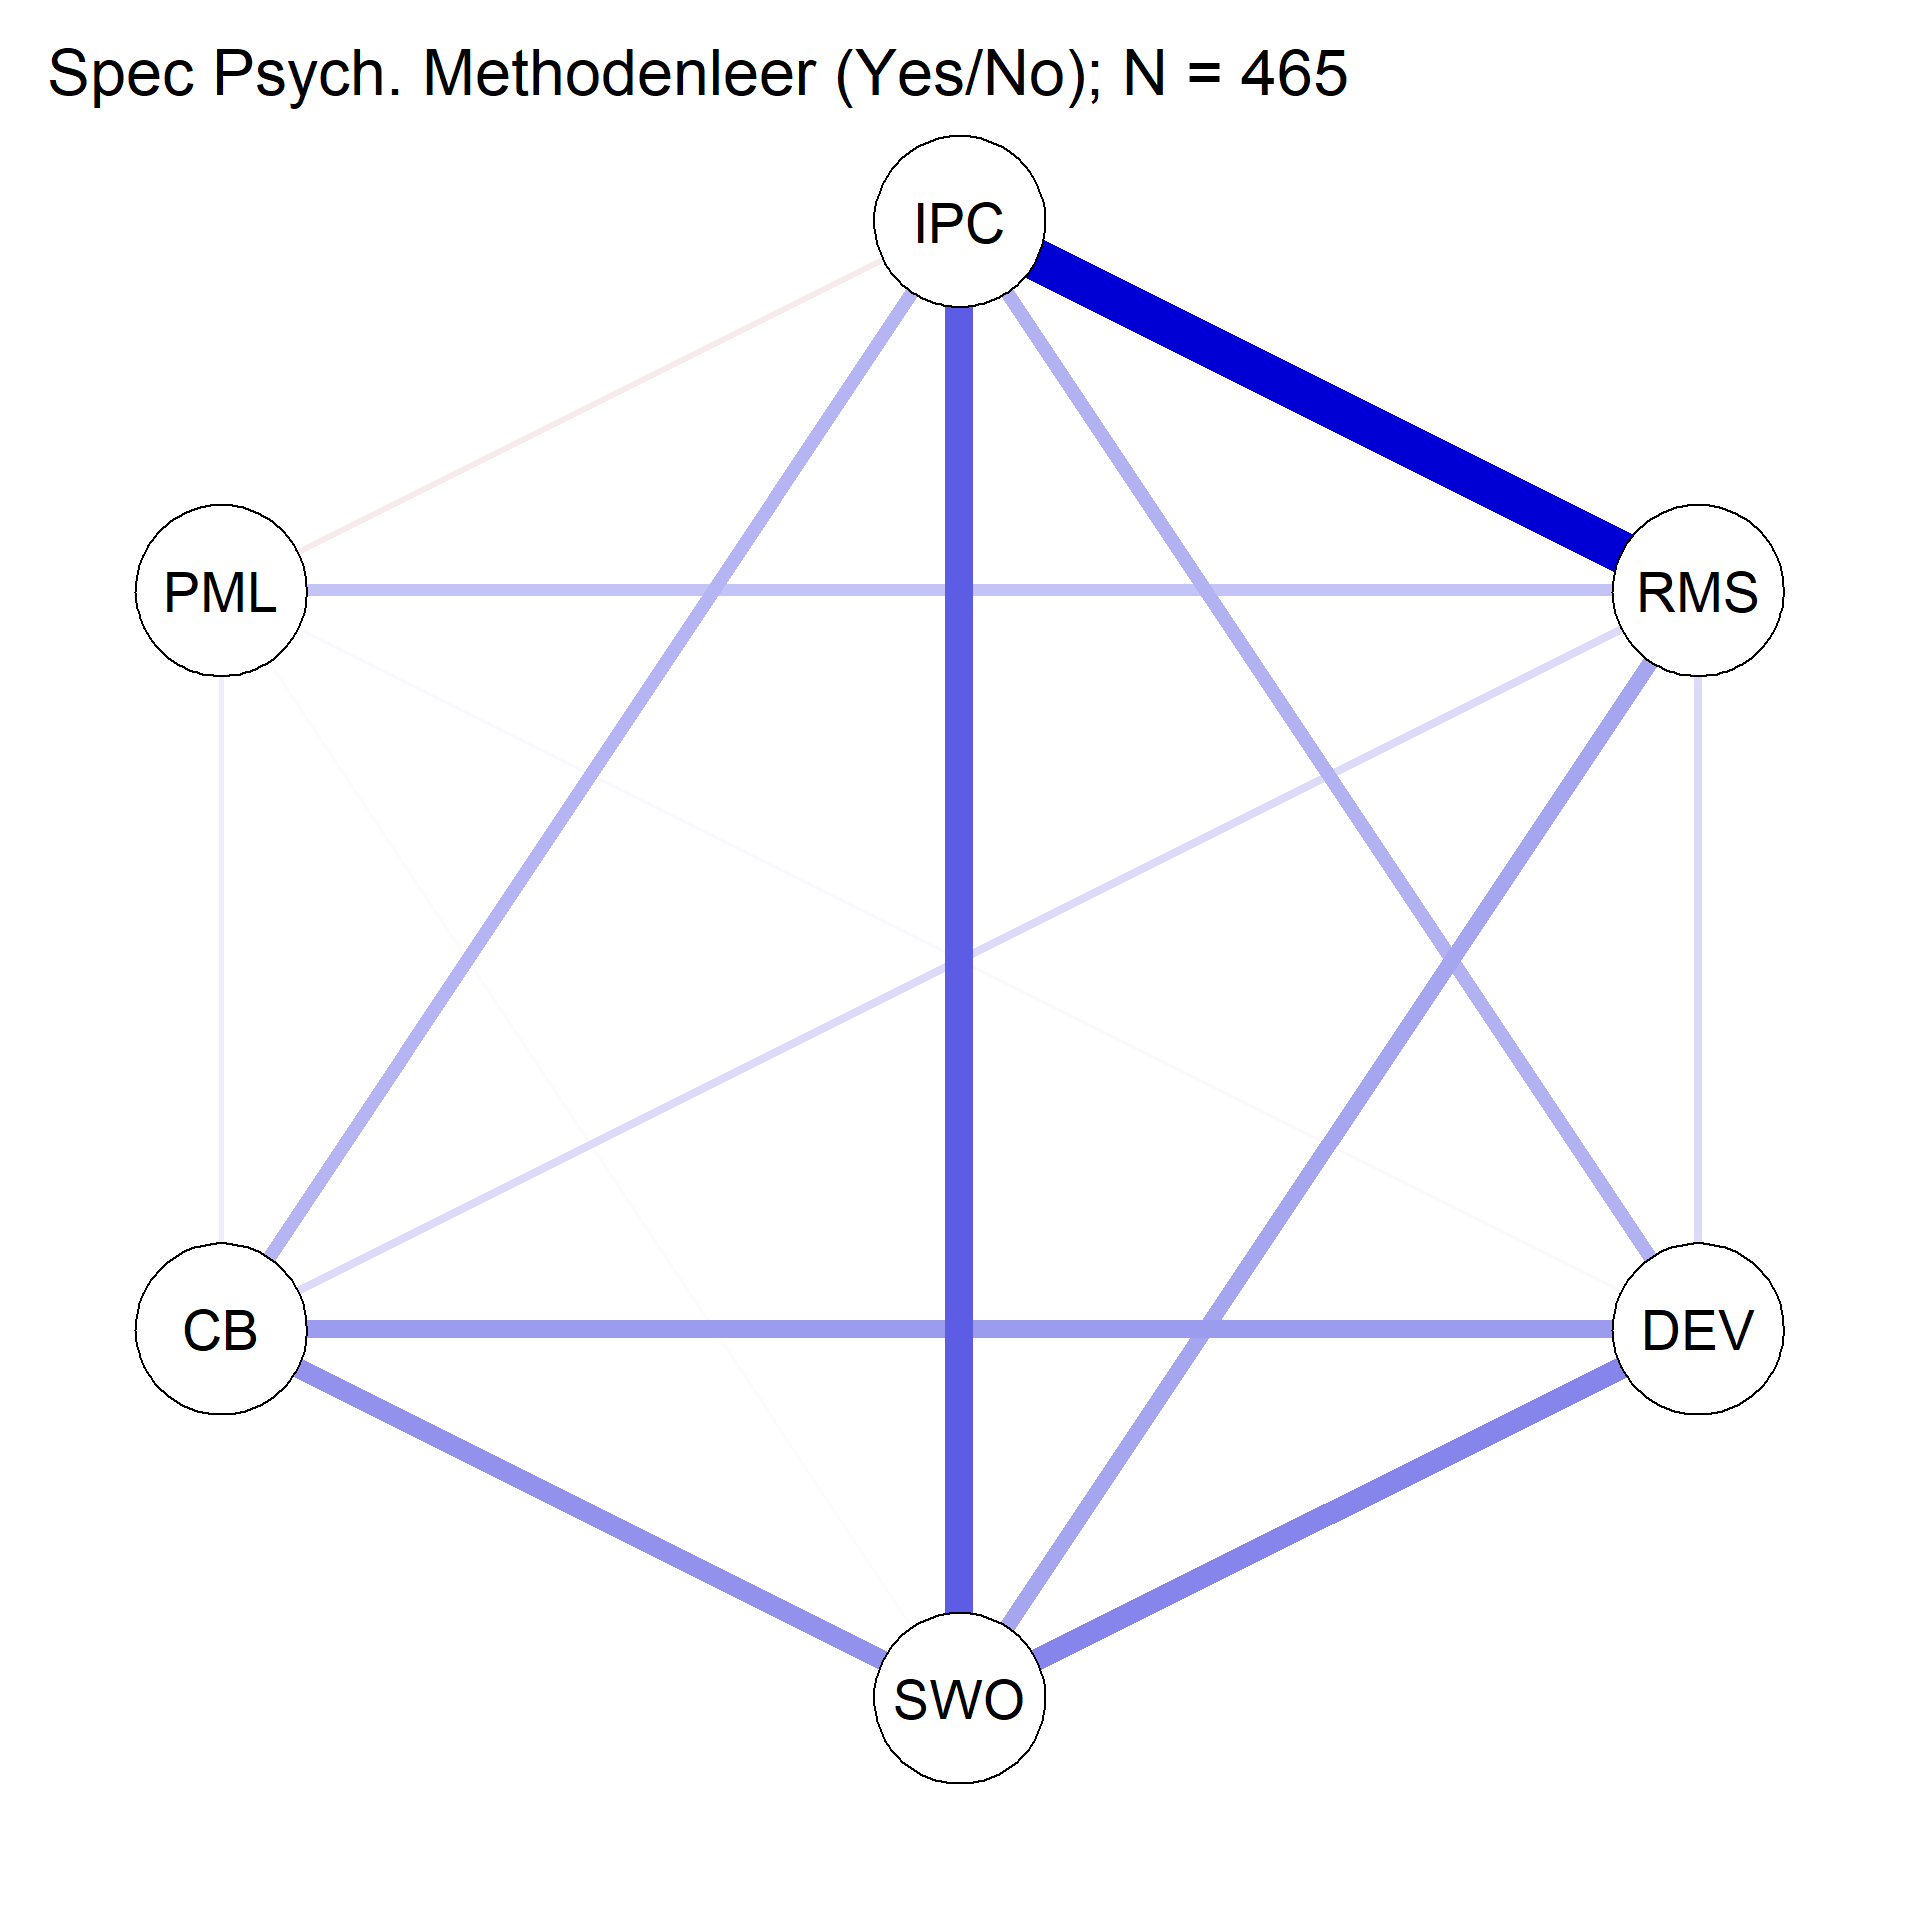
\includegraphics{2021_IDDC_Final-Report_Group-7_files/figure-latex/unnamed-chunk-19-1.pdf}

\begin{Shaded}
\begin{Highlighting}[]
\NormalTok{nCores <-}\StringTok{ }\NormalTok{parallel}\OperatorTok{::}\KeywordTok{detectCores}\NormalTok{()}

\KeywordTok{set.seed}\NormalTok{(}\DecValTok{222}\NormalTok{)}

\CommentTok{# Non-Parametric Bootstrap}
\NormalTok{bootNonParametric <-}\StringTok{ }\KeywordTok{bootnet}\NormalTok{(network,}
                             \DataTypeTok{nBoots =} \DecValTok{1000}\NormalTok{,}
                             \DataTypeTok{nCores =}\NormalTok{ nCores }\OperatorTok{-}\StringTok{ }\DecValTok{1}\NormalTok{)}
\CommentTok{# Case-Drop Bootstrap}
\NormalTok{bootCaseDrop <-}\StringTok{ }\KeywordTok{bootnet}\NormalTok{(network,}
                        \DataTypeTok{nBoots =} \DecValTok{1000}\NormalTok{,}
                        \DataTypeTok{nCores =}\NormalTok{ nCores }\OperatorTok{-}\StringTok{ }\DecValTok{1}\NormalTok{,}
                        \DataTypeTok{type =} \StringTok{"case"}\NormalTok{,}
                        \DataTypeTok{statistics =} \KeywordTok{c}\NormalTok{(}\StringTok{"Strength"}\NormalTok{, }\StringTok{"Closeness"}\NormalTok{, }\StringTok{"Betweenness"}\NormalTok{))}
\end{Highlighting}
\end{Shaded}

\begin{Shaded}
\begin{Highlighting}[]
\CommentTok{# Plot Edge Accuracy Non-Parametric Bootstrap}
\KeywordTok{plot}\NormalTok{(bootNonParametric,}
     \DataTypeTok{order =} \StringTok{"sample"}\NormalTok{,}
     \DataTypeTok{labels =} \OtherTok{FALSE}\NormalTok{)}
\end{Highlighting}
\end{Shaded}

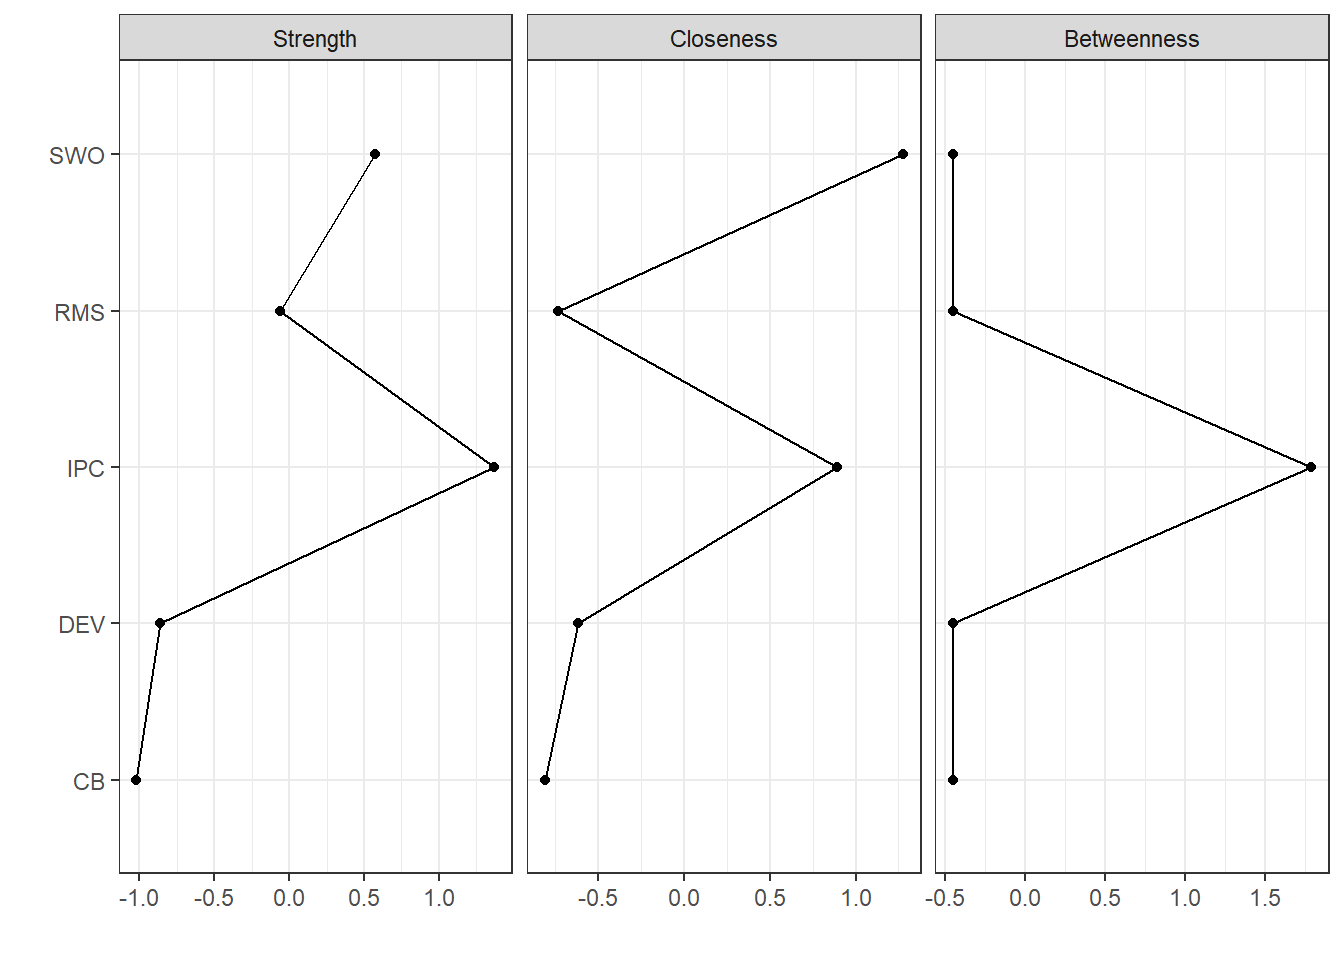
\includegraphics{2021_IDDC_Final-Report_Group-7_files/figure-latex/unnamed-chunk-21-1.pdf}

\begin{Shaded}
\begin{Highlighting}[]
\CommentTok{# Plot Edge Differences Non-Parametric Bootstrap}
\KeywordTok{plot}\NormalTok{(bootNonParametric,}
     \DataTypeTok{plot =} \StringTok{"difference"}\NormalTok{,}
     \DataTypeTok{onlyNonZero=} \OtherTok{TRUE}\NormalTok{,}
     \DataTypeTok{order =} \StringTok{"sample"}\NormalTok{)}
\end{Highlighting}
\end{Shaded}

\includegraphics{2021_IDDC_Final-Report_Group-7_files/figure-latex/unnamed-chunk-21-2.pdf}

\begin{Shaded}
\begin{Highlighting}[]
\CommentTok{# Plot Centrality Accuracy Case-Drop Bootstrap}
\KeywordTok{plot}\NormalTok{(bootCaseDrop,}
     \DataTypeTok{statistics =} \KeywordTok{c}\NormalTok{(}\StringTok{"Strength"}\NormalTok{, }\StringTok{"Closeness"}\NormalTok{, }\StringTok{"Betweenness"}\NormalTok{))}
\end{Highlighting}
\end{Shaded}

\includegraphics{2021_IDDC_Final-Report_Group-7_files/figure-latex/unnamed-chunk-21-3.pdf}

\begin{Shaded}
\begin{Highlighting}[]
\CommentTok{# CS-Coefficient}
\KeywordTok{corStability}\NormalTok{(bootCaseDrop)}
\end{Highlighting}
\end{Shaded}

\begin{verbatim}
## === Correlation Stability Analysis === 
## 
## Sampling levels tested:
##    nPerson Drop%   n
## 1      116  75.1 102
## 2      152  67.3 100
## 3      189  59.4 109
## 4      225  51.6  87
## 5      261  43.9 105
## 6      297  36.1 105
## 7      333  28.4 100
## 8      369  20.6 102
## 9      406  12.7  88
## 10     442   4.9 102
## 
## Maximum drop proportions to retain correlation of 0.7 in at least 95% of the samples:
## 
## betweenness: 0.049 (CS-coefficient is lowest level tested)
##   - For more accuracy, run bootnet(..., caseMin = 0, caseMax = 0.127) 
## 
## closeness: 0.516 
##   - For more accuracy, run bootnet(..., caseMin = 0.439, caseMax = 0.594) 
## 
## strength: 0.751 (CS-coefficient is highest level tested)
##   - For more accuracy, run bootnet(..., caseMin = 0.673, caseMax = 1) 
## 
## Accuracy can also be increased by increasing both 'nBoots' and 'caseN'.
\end{verbatim}

\begin{Shaded}
\begin{Highlighting}[]
\CommentTok{# Difference Test}
\KeywordTok{plot}\NormalTok{(bootCaseDrop, }\StringTok{"strength"}\NormalTok{)}
\end{Highlighting}
\end{Shaded}

\includegraphics{2021_IDDC_Final-Report_Group-7_files/figure-latex/unnamed-chunk-21-4.pdf}

\hypertarget{stability-checks-for-clinical-vs-non-clinical}{%
\subparagraph{Stability Checks for Clinical vs
Non-Clinical}\label{stability-checks-for-clinical-vs-non-clinical}}

\begin{Shaded}
\begin{Highlighting}[]
\CommentTok{# Create a subset for all students who have specialized in clinical psychology}
\NormalTok{dataClin <-}\StringTok{ }\NormalTok{data_wide[data_wide}\OperatorTok{$}\NormalTok{Specialization }\OperatorTok{==}\StringTok{ "Spec Klinische Psychologie"}\NormalTok{,]}

\CommentTok{# Create a subset for all students who have not specialized in clinical psychology}
\NormalTok{dataNotClin <-}\StringTok{ }\NormalTok{data_wide[data_wide}\OperatorTok{$}\NormalTok{Specialization }\OperatorTok{!=}\StringTok{ "Spec Klinische Psychologie"}\NormalTok{,]}
\end{Highlighting}
\end{Shaded}

\begin{Shaded}
\begin{Highlighting}[]
\CommentTok{# Estimating networks for both created subsets}
\NormalTok{networkCLIN <-}\StringTok{ }\KeywordTok{estimateNetwork}\NormalTok{(dataClin[,}\OperatorTok{-}\KeywordTok{c}\NormalTok{(}\DecValTok{1}\OperatorTok{:}\DecValTok{2}\NormalTok{)],}
                               \DataTypeTok{default =} \StringTok{"pcor"}\NormalTok{,}
                               \DataTypeTok{corMethod =} \StringTok{"spearman"}\NormalTok{)}

\NormalTok{networkNotCLIN <-}\StringTok{ }\KeywordTok{estimateNetwork}\NormalTok{(dataNotClin[,}\OperatorTok{-}\KeywordTok{c}\NormalTok{(}\DecValTok{1}\OperatorTok{:}\DecValTok{2}\NormalTok{)],}
                               \DataTypeTok{default =} \StringTok{"pcor"}\NormalTok{,}
                               \DataTypeTok{corMethod =} \StringTok{"spearman"}\NormalTok{)}
\end{Highlighting}
\end{Shaded}

\begin{Shaded}
\begin{Highlighting}[]
\CommentTok{# Visualising the estimated network}
\KeywordTok{qgraph}\NormalTok{(networkCLIN}\OperatorTok{$}\NormalTok{graph,}
       \DataTypeTok{layout =} \StringTok{"circle"}\NormalTok{,}
       \DataTypeTok{theme =} \StringTok{"colorblind"}\NormalTok{,}
       \DataTypeTok{title.cex =} \DecValTok{2}\NormalTok{,}
       \DataTypeTok{title =} \KeywordTok{paste}\NormalTok{(}\StringTok{"Spec Klinische Psychologie; N ="}\NormalTok{, }\KeywordTok{nrow}\NormalTok{(dataClin)))}
\end{Highlighting}
\end{Shaded}

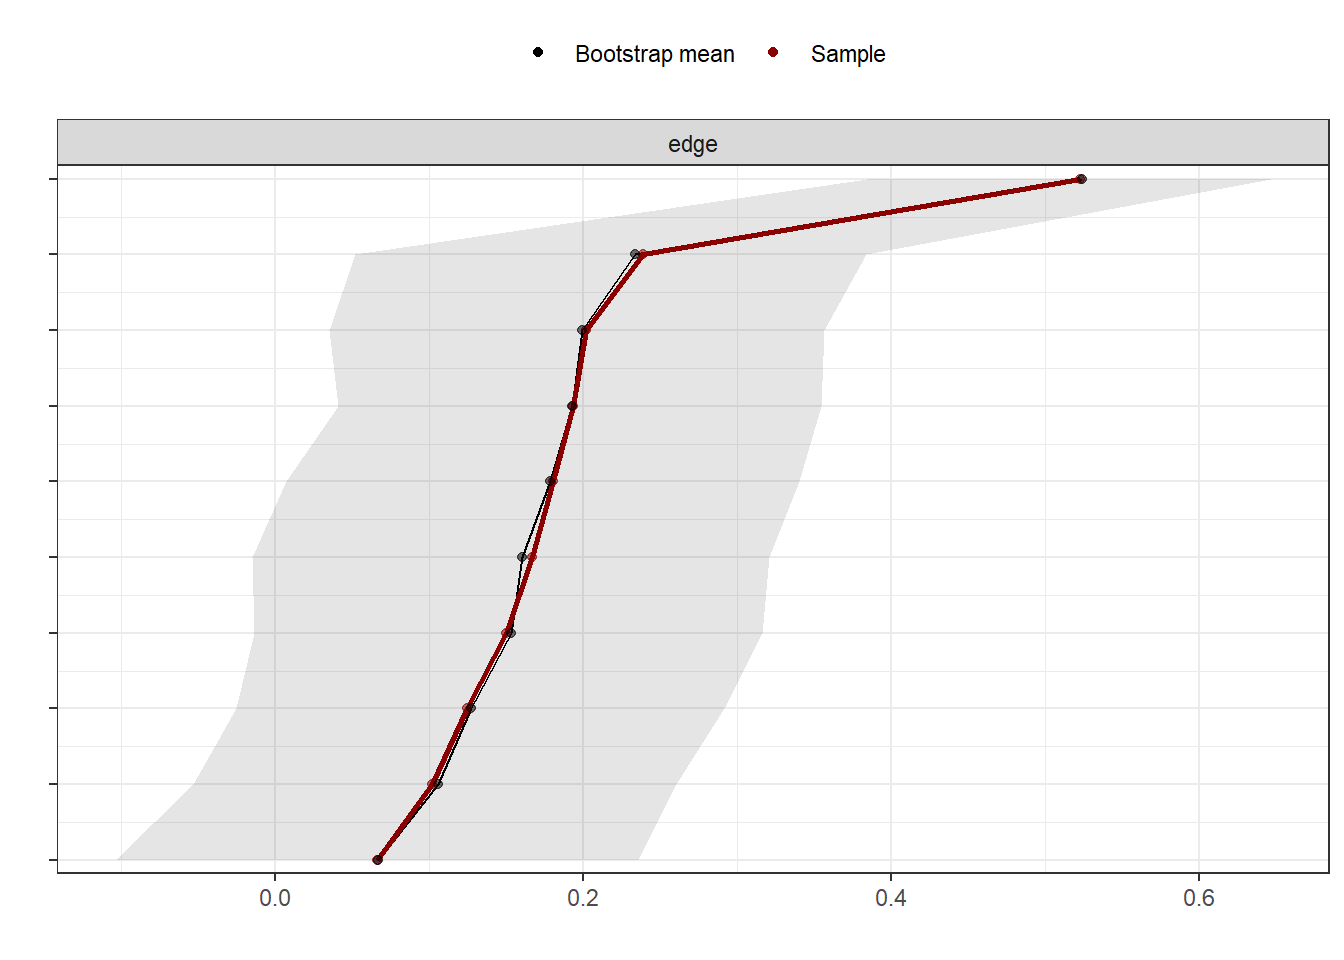
\includegraphics{2021_IDDC_Final-Report_Group-7_files/figure-latex/unnamed-chunk-24-1.pdf}

\begin{Shaded}
\begin{Highlighting}[]
\KeywordTok{qgraph}\NormalTok{(networkNotCLIN}\OperatorTok{$}\NormalTok{graph,}
       \DataTypeTok{layout =} \StringTok{"circle"}\NormalTok{,}
       \DataTypeTok{theme =} \StringTok{"colorblind"}\NormalTok{,}
       \DataTypeTok{title.cex =} \DecValTok{2}\NormalTok{,}
       \DataTypeTok{title =} \KeywordTok{paste}\NormalTok{(}\StringTok{"Not Spec Klinische Psychologie; N ="}\NormalTok{, }\KeywordTok{nrow}\NormalTok{(dataNotClin)))}
\end{Highlighting}
\end{Shaded}

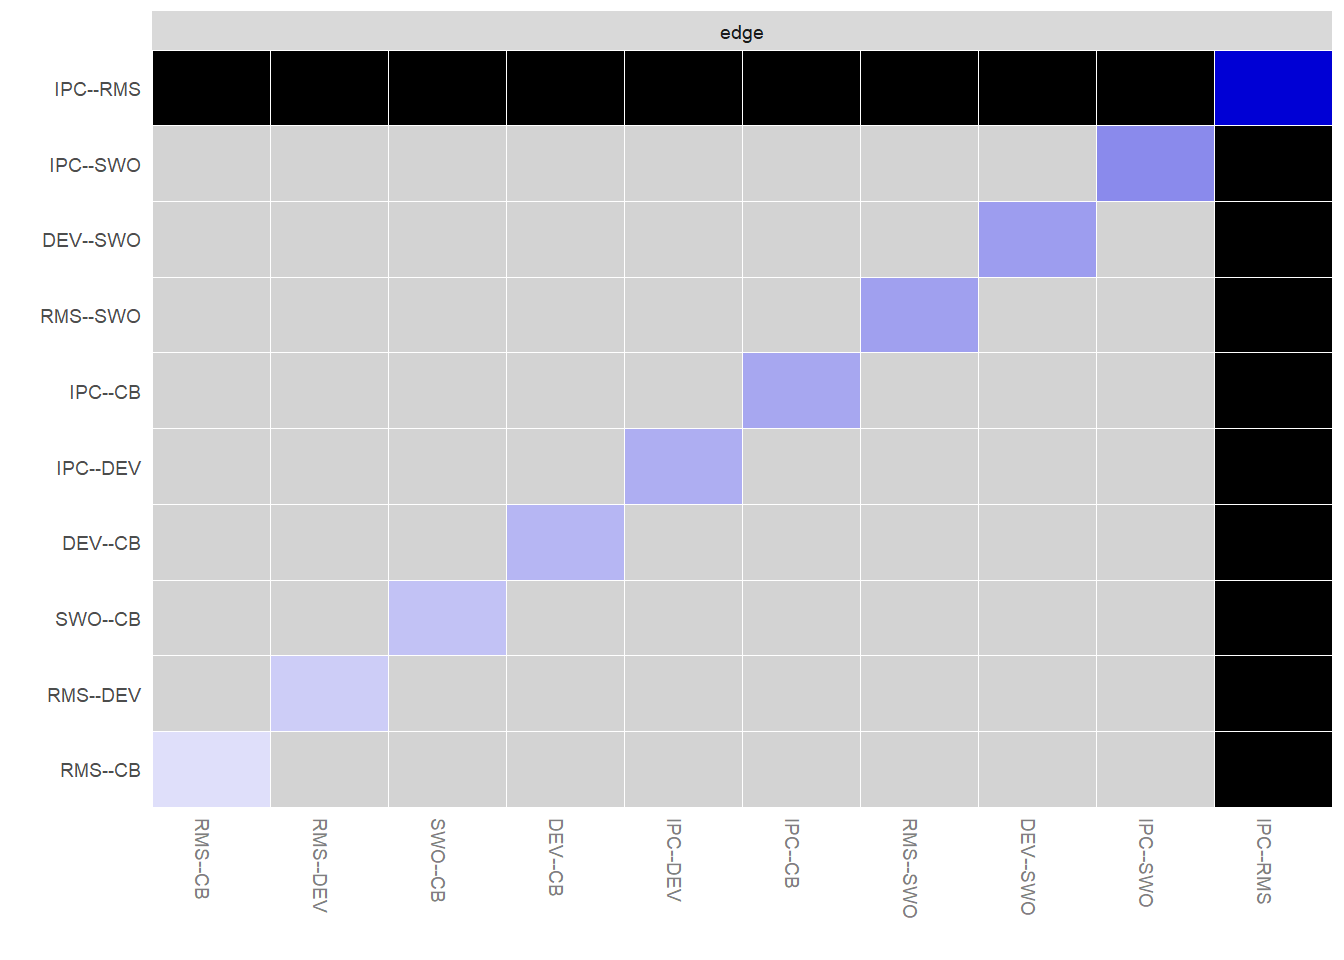
\includegraphics{2021_IDDC_Final-Report_Group-7_files/figure-latex/unnamed-chunk-24-2.pdf}

\begin{Shaded}
\begin{Highlighting}[]
\CommentTok{# Plot the centrality estimates}
\KeywordTok{centralityPlot}\NormalTok{(}\KeywordTok{list}\NormalTok{(}\DataTypeTok{Clinical =}\NormalTok{ networkCLIN,}
                    \StringTok{`}\DataTypeTok{Not Clinical}\StringTok{`}\NormalTok{ =}\StringTok{ }\NormalTok{networkNotCLIN),}
               \DataTypeTok{theme_bw =} \OtherTok{TRUE}\NormalTok{,}
               \DataTypeTok{include =} \KeywordTok{c}\NormalTok{(}\StringTok{"Strength"}\NormalTok{,}
                           \StringTok{"Closeness"}\NormalTok{,}
                           \StringTok{"Betweenness"}\NormalTok{))}
\end{Highlighting}
\end{Shaded}

\includegraphics{2021_IDDC_Final-Report_Group-7_files/figure-latex/unnamed-chunk-25-1.pdf}

\hypertarget{network-comparison-test-for-clinical-vs-non-clinical}{%
\subparagraph{Network Comparison Test for Clinical vs
Non-Clinical}\label{network-comparison-test-for-clinical-vs-non-clinical}}

\begin{Shaded}
\begin{Highlighting}[]
\KeywordTok{set.seed}\NormalTok{(}\DecValTok{45}\NormalTok{)}

\CommentTok{# Comparing the network structures of the clinical and non-clinical network estimates}
\NormalTok{NCT <-}\StringTok{ }
\NormalTok{NetworkComparisonTest}\OperatorTok{::}\KeywordTok{NCT}\NormalTok{(networkCLIN, networkNotCLIN,}
                           \DataTypeTok{it =} \DecValTok{2000}\NormalTok{,}
                           \DataTypeTok{test.edges =} \OtherTok{TRUE}\NormalTok{,}
                           \DataTypeTok{edges =} \StringTok{"all"}\NormalTok{,}
                           \DataTypeTok{progressbar =} \OtherTok{FALSE}\NormalTok{)}

\CommentTok{# Results for the network comparison test}
\NormalTok{NCT}
\end{Highlighting}
\end{Shaded}

\begin{verbatim}
## 
##  NETWORK INVARIANCE TEST 
##  Test statistic M:  0.1066753 
##  p-value 0.904 
## 
##  GLOBAL STRENGTH INVARIANCE TEST 
##  Global strength per group:  2.036025 1.927125 
##  Test statistic S:  0.1089002 
##  p-value 0.1875 
## 
##  EDGE INVARIANCE TEST 
## 
##    Var1 Var2 p-value
## 6   IPC  RMS   0.893
## 11  IPC  DEV   0.501
## 12  RMS  DEV   0.996
## 16  IPC  SWO   0.877
## 17  RMS  SWO   0.233
## 18  DEV  SWO   0.803
## 21  IPC   CB   0.748
## 22  RMS   CB   0.751
## 23  DEV   CB   0.428
## 24  SWO   CB   0.684
## 
##  CENTRALITY INVARIANCE TEST 
##  
## NULL
\end{verbatim}

\begin{Shaded}
\begin{Highlighting}[]
\CommentTok{# Returns the edges that differ significantly between both networks}
\NormalTok{NCT}\OperatorTok{$}\NormalTok{einv.pvals }\OperatorTok\StringTok{ }
\StringTok{    }\KeywordTok{filter}\NormalTok{(}\StringTok{`}\DataTypeTok{p-value}\StringTok{`} \OperatorTok{<=}\StringTok{ }\FloatTok{.05}\NormalTok{)}
\end{Highlighting}
\end{Shaded}

\begin{verbatim}
## [1] Var1    Var2    p-value
## <0 rows> (or 0-length row.names)
\end{verbatim}

\hypertarget{stability-checks-for-clinical-vs-non-clinical-1}{%
\subparagraph{Stability Checks for Clinical vs
Non-Clinical}\label{stability-checks-for-clinical-vs-non-clinical-1}}

\begin{Shaded}
\begin{Highlighting}[]
\NormalTok{nCores <-}\StringTok{ }\NormalTok{parallel}\OperatorTok{::}\KeywordTok{detectCores}\NormalTok{()}

\KeywordTok{set.seed}\NormalTok{(}\DecValTok{555}\NormalTok{)}

\CommentTok{# Non-Parametric Bootstrap}
\NormalTok{bootNonParametricCLIN <-}\StringTok{ }\KeywordTok{bootnet}\NormalTok{(networkCLIN,}
                             \DataTypeTok{nBoots =} \DecValTok{1000}\NormalTok{,}
                             \DataTypeTok{nCores =}\NormalTok{ nCores }\OperatorTok{-}\StringTok{ }\DecValTok{1}\NormalTok{)}
\CommentTok{# Case-Drop Bootstrap}
\NormalTok{bootCaseDropCLIN <-}\StringTok{ }\KeywordTok{bootnet}\NormalTok{(networkCLIN,}
                        \DataTypeTok{nBoots =} \DecValTok{1000}\NormalTok{,}
                        \DataTypeTok{nCores =}\NormalTok{ nCores }\OperatorTok{-}\StringTok{ }\DecValTok{1}\NormalTok{,}
                        \DataTypeTok{type =} \StringTok{"case"}\NormalTok{,}
                        \DataTypeTok{statistics =} \KeywordTok{c}\NormalTok{(}\StringTok{"Strength"}\NormalTok{, }\StringTok{"Closeness"}\NormalTok{, }\StringTok{"Betweenness"}\NormalTok{))}
\end{Highlighting}
\end{Shaded}

\begin{Shaded}
\begin{Highlighting}[]
\CommentTok{# Plot Edge Accuracy Non-Parametric Bootstrap}
\KeywordTok{plot}\NormalTok{(bootNonParametricCLIN,}
     \DataTypeTok{order =} \StringTok{"sample"}\NormalTok{,}
     \DataTypeTok{labels =} \OtherTok{FALSE}\NormalTok{)}
\end{Highlighting}
\end{Shaded}

\includegraphics{2021_IDDC_Final-Report_Group-7_files/figure-latex/unnamed-chunk-28-1.pdf}

\begin{Shaded}
\begin{Highlighting}[]
\CommentTok{# Plot Edge Differences Non-Parametric Bootstrap}
\KeywordTok{plot}\NormalTok{(bootNonParametricCLIN,}
     \DataTypeTok{plot =} \StringTok{"difference"}\NormalTok{,}
     \DataTypeTok{onlyNonZero=} \OtherTok{TRUE}\NormalTok{,}
     \DataTypeTok{order =} \StringTok{"sample"}\NormalTok{)}
\end{Highlighting}
\end{Shaded}

\includegraphics{2021_IDDC_Final-Report_Group-7_files/figure-latex/unnamed-chunk-28-2.pdf}

\begin{Shaded}
\begin{Highlighting}[]
\CommentTok{# Plot Centrality Accuracy Case-Drop Bootstrap}
\KeywordTok{plot}\NormalTok{(bootCaseDropCLIN,}
     \DataTypeTok{statistics =} \KeywordTok{c}\NormalTok{(}\StringTok{"Strength"}\NormalTok{, }\StringTok{"Closeness"}\NormalTok{, }\StringTok{"Betweenness"}\NormalTok{))}
\end{Highlighting}
\end{Shaded}

\includegraphics{2021_IDDC_Final-Report_Group-7_files/figure-latex/unnamed-chunk-28-3.pdf}

\begin{Shaded}
\begin{Highlighting}[]
\CommentTok{# CS-Coefficient}
\KeywordTok{corStability}\NormalTok{(bootCaseDropCLIN)}
\end{Highlighting}
\end{Shaded}

\begin{verbatim}
## === Correlation Stability Analysis === 
## 
## Sampling levels tested:
##    nPerson Drop%   n
## 1       50  75.2 108
## 2       66  67.3 108
## 3       82  59.4 104
## 4       98  51.5 108
## 5      113  44.1 108
## 6      129  36.1 110
## 7      145  28.2  82
## 8      160  20.8  84
## 9      176  12.9  85
## 10     192   5.0 103
## 
## Maximum drop proportions to retain correlation of 0.7 in at least 95% of the samples:
## 
## betweenness: 0.05 (CS-coefficient is lowest level tested)
##   - For more accuracy, run bootnet(..., caseMin = 0, caseMax = 0.129) 
## 
## closeness: 0.129 
##   - For more accuracy, run bootnet(..., caseMin = 0.05, caseMax = 0.208) 
## 
## strength: 0.441 
##   - For more accuracy, run bootnet(..., caseMin = 0.361, caseMax = 0.515) 
## 
## Accuracy can also be increased by increasing both 'nBoots' and 'caseN'.
\end{verbatim}

\begin{Shaded}
\begin{Highlighting}[]
\CommentTok{# Difference Test}
\KeywordTok{plot}\NormalTok{(bootNonParametricCLIN, }\StringTok{"strength"}\NormalTok{)}
\end{Highlighting}
\end{Shaded}

\includegraphics{2021_IDDC_Final-Report_Group-7_files/figure-latex/unnamed-chunk-28-4.pdf}

\begin{Shaded}
\begin{Highlighting}[]
\NormalTok{nCores <-}\StringTok{ }\NormalTok{parallel}\OperatorTok{::}\KeywordTok{detectCores}\NormalTok{()}

\KeywordTok{set.seed}\NormalTok{(}\DecValTok{444}\NormalTok{)}

\CommentTok{# Non-Parametric Bootstrap}
\NormalTok{bootNonParametricNotCLIN <-}\StringTok{ }\KeywordTok{bootnet}\NormalTok{(networkNotCLIN,}
                             \DataTypeTok{nBoots =} \DecValTok{1000}\NormalTok{,}
                             \DataTypeTok{nCores =}\NormalTok{ nCores }\OperatorTok{-}\StringTok{ }\DecValTok{1}\NormalTok{)}
\CommentTok{# Case-Drop Bootstrap}
\NormalTok{bootCaseDropNotCLIN<-}\StringTok{ }\KeywordTok{bootnet}\NormalTok{(networkNotCLIN,}
                        \DataTypeTok{nBoots =} \DecValTok{1000}\NormalTok{,}
                        \DataTypeTok{nCores =}\NormalTok{ nCores }\OperatorTok{-}\StringTok{ }\DecValTok{1}\NormalTok{,}
                        \DataTypeTok{type =} \StringTok{"case"}\NormalTok{,}
                        \DataTypeTok{statistics =} \KeywordTok{c}\NormalTok{(}\StringTok{"Strength"}\NormalTok{, }\StringTok{"Closeness"}\NormalTok{, }\StringTok{"Betweenness"}\NormalTok{))}
\end{Highlighting}
\end{Shaded}

\begin{Shaded}
\begin{Highlighting}[]
\CommentTok{# Plot Edge Accuracy Non-Parametric Bootstrap}
\KeywordTok{plot}\NormalTok{(bootNonParametricNotCLIN,}
     \DataTypeTok{order =} \StringTok{"sample"}\NormalTok{,}
     \DataTypeTok{labels =} \OtherTok{FALSE}\NormalTok{)}
\end{Highlighting}
\end{Shaded}

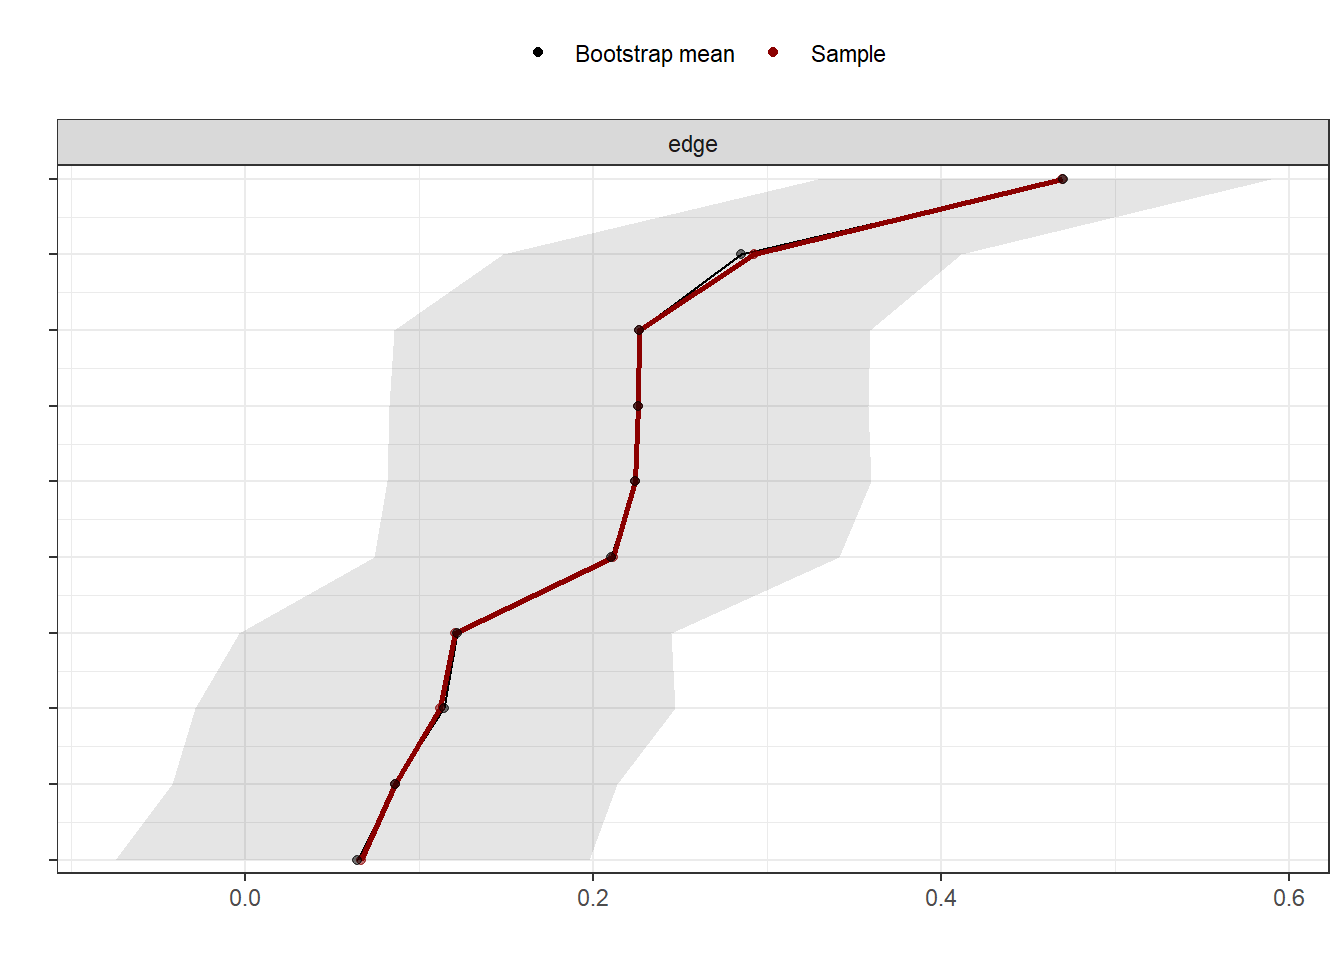
\includegraphics{2021_IDDC_Final-Report_Group-7_files/figure-latex/unnamed-chunk-30-1.pdf}

\begin{Shaded}
\begin{Highlighting}[]
\CommentTok{# Plot Edge Differences Non-Parametric Bootstrap}
\KeywordTok{plot}\NormalTok{(bootNonParametricNotCLIN,}
     \DataTypeTok{plot =} \StringTok{"difference"}\NormalTok{,}
     \DataTypeTok{onlyNonZero=} \OtherTok{TRUE}\NormalTok{,}
     \DataTypeTok{order =} \StringTok{"sample"}\NormalTok{)}
\end{Highlighting}
\end{Shaded}

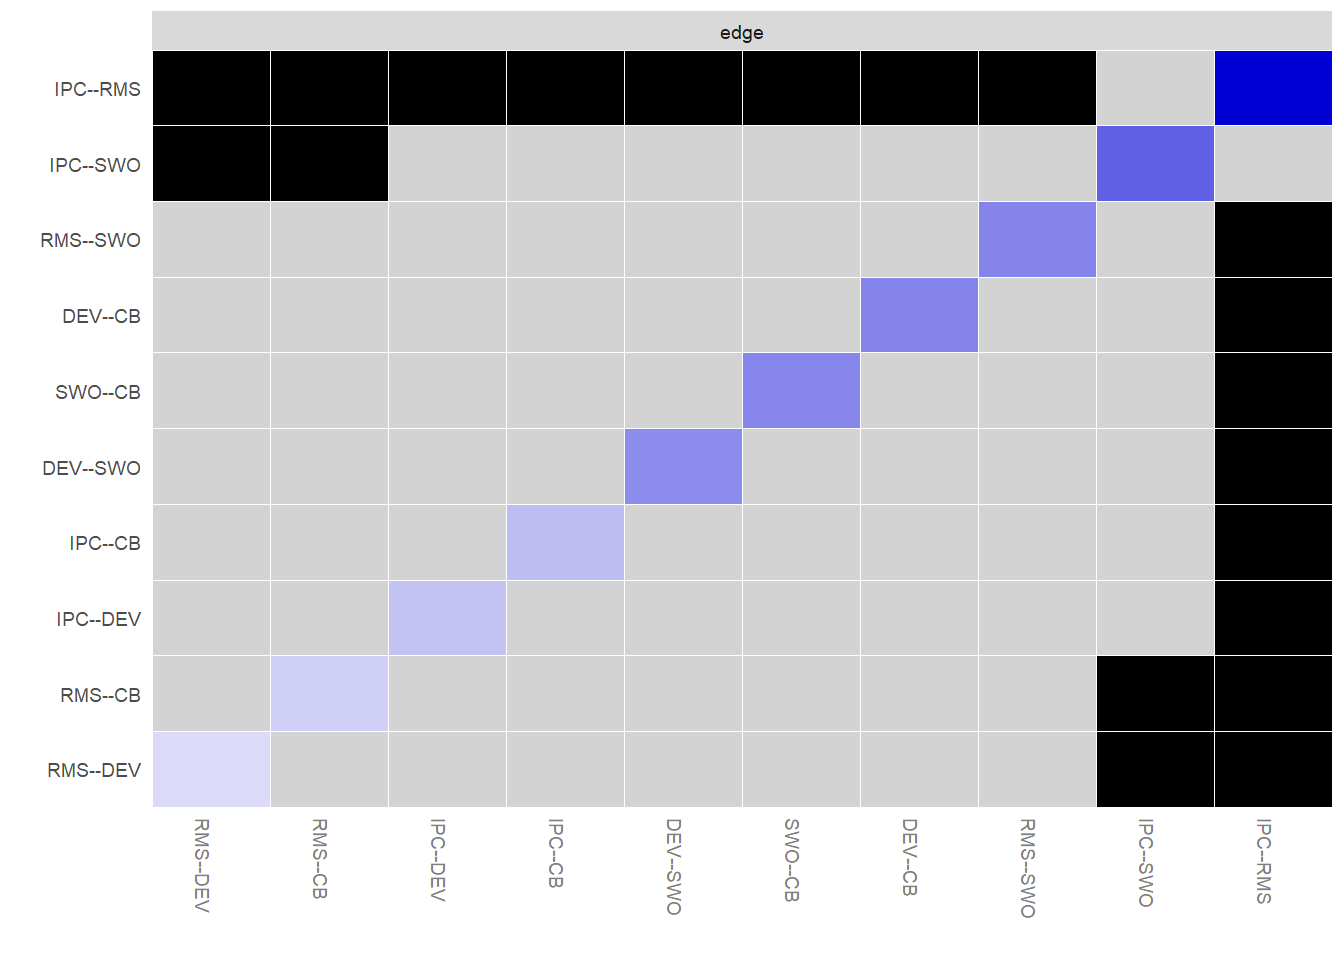
\includegraphics{2021_IDDC_Final-Report_Group-7_files/figure-latex/unnamed-chunk-30-2.pdf}

\begin{Shaded}
\begin{Highlighting}[]
\CommentTok{# Plot Centrality Accuracy Case-Drop Bootstrap}
\KeywordTok{plot}\NormalTok{(bootCaseDropNotCLIN,}
     \DataTypeTok{statistics =} \KeywordTok{c}\NormalTok{(}\StringTok{"Strength"}\NormalTok{, }\StringTok{"Closeness"}\NormalTok{, }\StringTok{"Betweenness"}\NormalTok{))}
\end{Highlighting}
\end{Shaded}

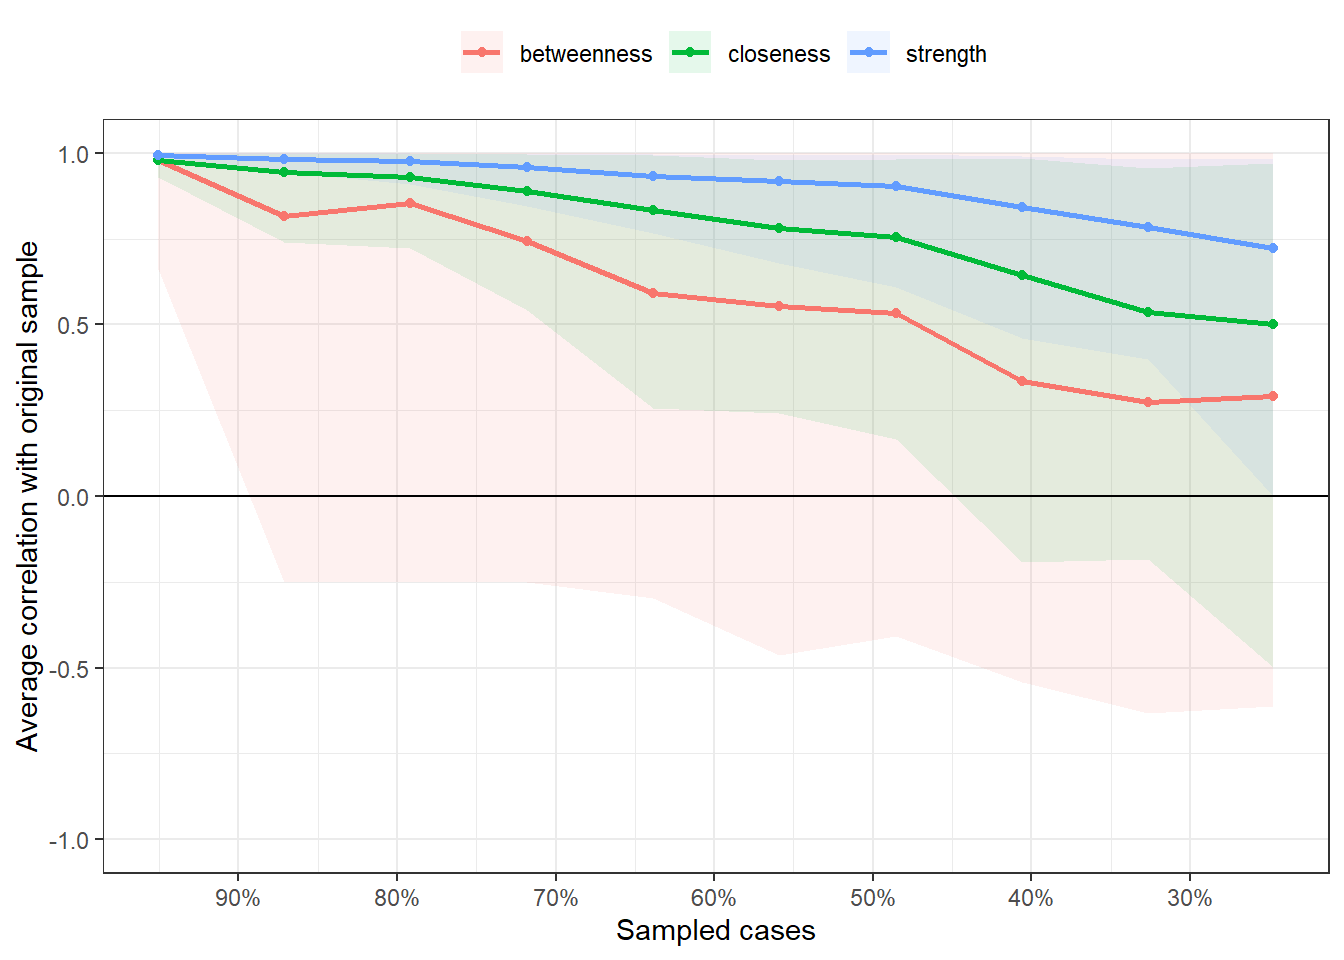
\includegraphics{2021_IDDC_Final-Report_Group-7_files/figure-latex/unnamed-chunk-30-3.pdf}

\begin{Shaded}
\begin{Highlighting}[]
\CommentTok{# CS-Coefficient}
\KeywordTok{corStability}\NormalTok{(bootCaseDropNotCLIN)}
\end{Highlighting}
\end{Shaded}

\begin{verbatim}
## === Correlation Stability Analysis === 
## 
## Sampling levels tested:
##    nPerson Drop%   n
## 1       66  74.9 117
## 2       86  67.3  98
## 3      107  59.3  94
## 4      127  51.7 104
## 5      148  43.7 103
## 6      168  36.1 107
## 7      188  28.5  85
## 8      209  20.5  90
## 9      229  12.9 116
## 10     250   4.9  86
## 
## Maximum drop proportions to retain correlation of 0.7 in at least 95% of the samples:
## 
## betweenness: 0.205 
##   - For more accuracy, run bootnet(..., caseMin = 0.129, caseMax = 0.285) 
## 
## closeness: 0.437 
##   - For more accuracy, run bootnet(..., caseMin = 0.361, caseMax = 0.517) 
## 
## strength: 0.593 
##   - For more accuracy, run bootnet(..., caseMin = 0.517, caseMax = 0.673) 
## 
## Accuracy can also be increased by increasing both 'nBoots' and 'caseN'.
\end{verbatim}

\begin{Shaded}
\begin{Highlighting}[]
\CommentTok{# Difference Test}
\KeywordTok{plot}\NormalTok{(bootNonParametricNotCLIN, }\StringTok{"strength"}\NormalTok{)}
\end{Highlighting}
\end{Shaded}

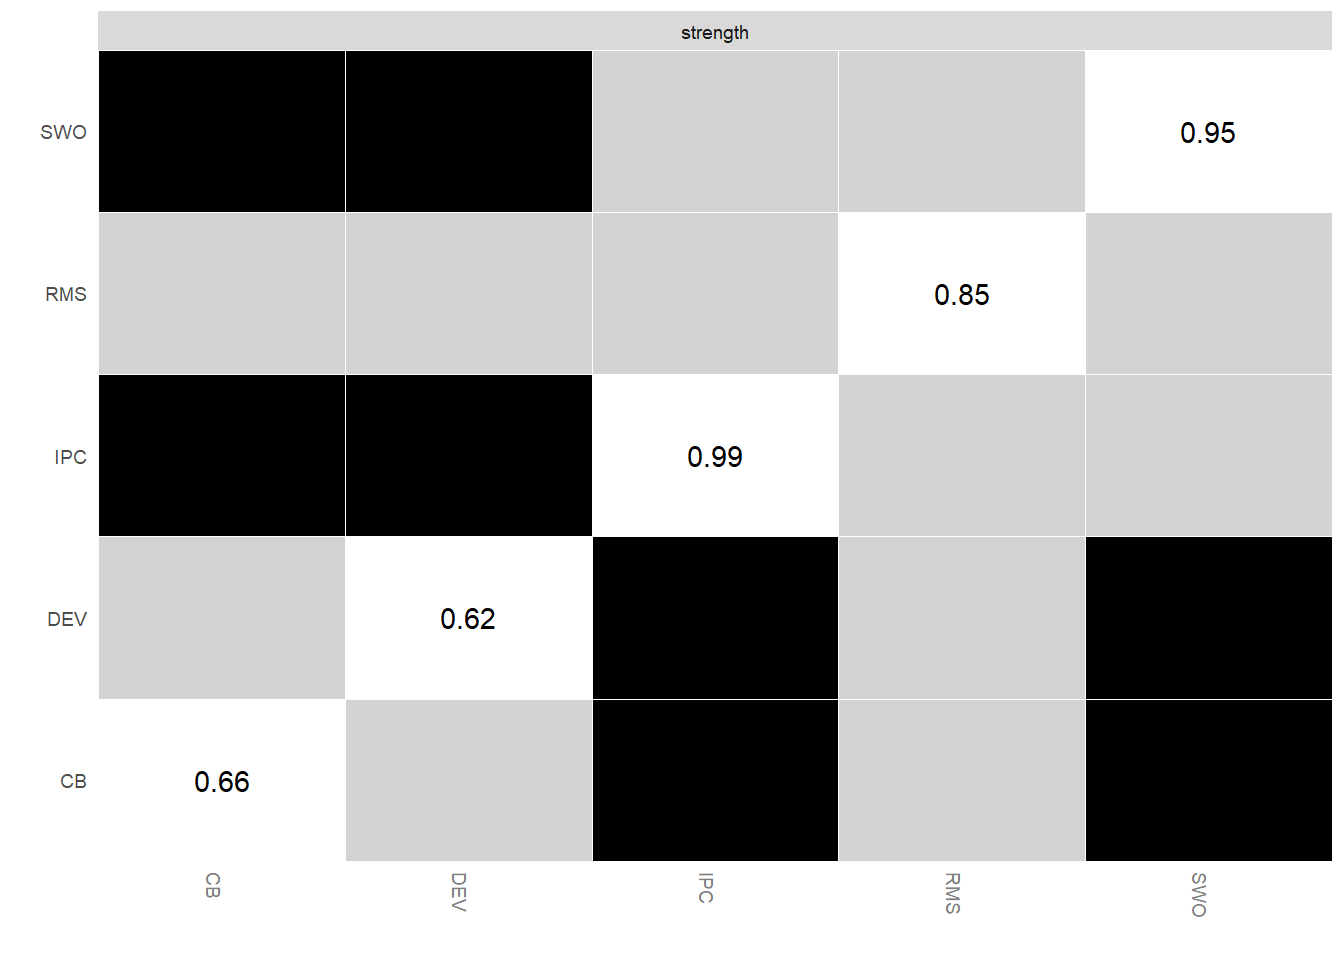
\includegraphics{2021_IDDC_Final-Report_Group-7_files/figure-latex/unnamed-chunk-30-4.pdf}

\hypertarget{mixed-graphical-models-mgms}{%
\subsection{Mixed Graphical Models
(MGMs)}\label{mixed-graphical-models-mgms}}

\begin{Shaded}
\begin{Highlighting}[]
\KeywordTok{library}\NormalTok{(mgm)}

\CommentTok{# Transform long grade data into wide format}
\NormalTok{generate_wide_grades <-}\StringTok{ }\ControlFlowTok{function}\NormalTok{ (data, grade_column) \{}
\NormalTok{  data }\OperatorTok
\StringTok{    }\KeywordTok{mutate}\NormalTok{(}
      \DataTypeTok{course_abb =} \KeywordTok{recode}\NormalTok{(course_id, }\OperatorTok{!!!}\NormalTok{course_abbrevations)}
\NormalTok{    ) }\OperatorTok\StringTok{ }
\StringTok{    }\KeywordTok{pivot_wider}\NormalTok{(}
      \DataTypeTok{id_cols =}\NormalTok{ student_id,}
      \DataTypeTok{names_from =}\NormalTok{ course_abb,}
      
      \CommentTok{# Use variable to assign grade column}
      \DataTypeTok{values_from =}\NormalTok{ grade_column}
\NormalTok{    ) }\OperatorTok\StringTok{ }
\StringTok{    }\CommentTok{# Add a column with specialisation info}
\StringTok{    }\KeywordTok{left_join}\NormalTok{(}
\NormalTok{      data }\OperatorTok
\StringTok{        }\KeywordTok{select}\NormalTok{(student_id, specialisation) }\OperatorTok
\StringTok{        }\KeywordTok{distinct}\NormalTok{(),}
      \DataTypeTok{by =} \StringTok{"student_id"}
\NormalTok{    )}
\NormalTok{\}}

\CommentTok{# Collect some info about columns}
\CommentTok{# This just needs to be a list of characters for each column indicating}
\CommentTok{# the type. Automated code here is just for flexibility.}
\NormalTok{extract_mgm_column_info <-}\StringTok{ }\NormalTok{. }\OperatorTok\StringTok{ }
\StringTok{  }\CommentTok{# Get only TRUE/FALSE whether columns are numeric}
\StringTok{  }\KeywordTok{summarise}\NormalTok{(}\KeywordTok{across}\NormalTok{(}\KeywordTok{everything}\NormalTok{(), is.numeric)) }\OperatorTok\StringTok{ }
\StringTok{  }\CommentTok{# Get into long format with column names and whether they are numeric in 2 columns}
\StringTok{  }\KeywordTok{pivot_longer}\NormalTok{(}
    \KeywordTok{everything}\NormalTok{(),}
    \DataTypeTok{names_to =} \StringTok{"column"}\NormalTok{,}
    \DataTypeTok{values_to =} \StringTok{"is_numeric"}
\NormalTok{  ) }\OperatorTok\StringTok{ }
\StringTok{  }\CommentTok{# Assign letters based on whether column is numeric or not}
\StringTok{  }\KeywordTok{mutate}\NormalTok{(}
    \DataTypeTok{column =} \KeywordTok{recode}\NormalTok{(column, }\DataTypeTok{specialisation =} \StringTok{"SPEC"}\NormalTok{),}
    \CommentTok{# Types for mgm}
    \CommentTok{# g: gaussian (normal dist.)}
    \CommentTok{# c: categorical}
    \CommentTok{# p: poisson (if skewed)}
    \DataTypeTok{type =} \KeywordTok{ifelse}\NormalTok{(is_numeric, }\StringTok{"g"}\NormalTok{, }\StringTok{"c"}\NormalTok{)}
\NormalTok{  )}
\end{Highlighting}
\end{Shaded}

\hypertarget{mgm-predicting-all-specializations-at-once}{%
\subsubsection{MGM Predicting all Specializations at
Once}\label{mgm-predicting-all-specializations-at-once}}

We first fit a mixed graphical model with contiuous gaussian nodes for
the course grades and a single categorical node for the different
specializations.

\begin{Shaded}
\begin{Highlighting}[]
\KeywordTok{set.seed}\NormalTok{(}\DecValTok{2021}\NormalTok{)}
\CommentTok{# ==== Preparate data for MGM ====}
\NormalTok{mgm_num_data <-}\StringTok{ }\NormalTok{data }\OperatorTok\StringTok{ }
\StringTok{  }\KeywordTok{generate_wide_grades}\NormalTok{(}\StringTok{"grade"}\NormalTok{) }\OperatorTok
\StringTok{  }\CommentTok{# Drop Student IDs}
\StringTok{  }\KeywordTok{select}\NormalTok{(}\OperatorTok{-}\NormalTok{student_id) }\OperatorTok\StringTok{ }
\StringTok{  }\CommentTok{# Drop all NAs (}\AlertTok{NOTE}\CommentTok{: this loses us about 2/3 of the data)}
\StringTok{  }\KeywordTok{na.omit}\NormalTok{()}

\NormalTok{column_info <-}\StringTok{ }\KeywordTok{extract_mgm_column_info}\NormalTok{(mgm_num_data)}

\CommentTok{# Transform categorical variables to integers}
\CommentTok{# mgm wants all data as numbers!}
\NormalTok{mgm_num_data_numeric <-}\StringTok{ }\NormalTok{mgm_num_data }\OperatorTok\StringTok{ }
\StringTok{  }\KeywordTok{mutate}\NormalTok{(}
    \DataTypeTok{specialisation =} \KeywordTok{as.numeric}\NormalTok{(}\KeywordTok{as.factor}\NormalTok{(specialisation))}
\NormalTok{  )}

\CommentTok{# V1: mgm package directly}
\NormalTok{trainidx <-}\StringTok{ }\KeywordTok{sample}\NormalTok{(}\KeywordTok{seq_len}\NormalTok{(}\KeywordTok{nrow}\NormalTok{(mgm_num_data)), }\DataTypeTok{size =} \KeywordTok{floor}\NormalTok{(.}\DecValTok{8} \OperatorTok{*}\StringTok{ }\KeywordTok{nrow}\NormalTok{(mgm_num_data)))}

\NormalTok{fit_mgm_num <-}\StringTok{ }\KeywordTok{mgm}\NormalTok{(}
  \DataTypeTok{data =}\NormalTok{ mgm_num_data_numeric[trainidx,],}
  \DataTypeTok{type =}\NormalTok{ column_info}\OperatorTok{$}\NormalTok{type}
\NormalTok{)}
\end{Highlighting}
\end{Shaded}

\begin{verbatim}
##   |                                                                              |                                                                      |   0%  |                                                                              |------------                                                          |  17%  |                                                                              |-----------------------                                               |  33%  |                                                                              |-----------------------------------                                   |  50%  |                                                                              |-----------------------------------------------                       |  67%  |                                                                              |----------------------------------------------------------            |  83%  |                                                                              |----------------------------------------------------------------------| 100%
## Note that the sign of parameter estimates is stored separately; see ?mgm
\end{verbatim}

\begin{Shaded}
\begin{Highlighting}[]
\CommentTok{# Predict the training data}
\NormalTok{prediction_mgm <-}\StringTok{ }\KeywordTok{predict}\NormalTok{(}
\NormalTok{  fit_mgm_num,}
  \DataTypeTok{data =}\NormalTok{ mgm_num_data_numeric[}\OperatorTok{-}\NormalTok{trainidx,],}
  \DataTypeTok{errorCat =} \KeywordTok{c}\NormalTok{(}\StringTok{"CC"}\NormalTok{,}\StringTok{"nCC"}\NormalTok{,}\StringTok{"CCmarg"}\NormalTok{),}
  \DataTypeTok{errorCon =} \KeywordTok{c}\NormalTok{(}\StringTok{"R2"}\NormalTok{)}
\NormalTok{)}

 \CommentTok{# Prediction error}
\NormalTok{prediction_mgm}\OperatorTok{$}\NormalTok{errors }\OperatorTok\StringTok{ }\NormalTok{knitr}\OperatorTok{::}\KeywordTok{kable}\NormalTok{()}
\end{Highlighting}
\end{Shaded}

\begin{longtable}[]{@{}lrrrr@{}}
\toprule
Variable & R2 & CC & nCC & CCmarg\tabularnewline
\midrule
\endhead
IPC & 0.682 & NA & NA & NA\tabularnewline
RMS & 0.581 & NA & NA & NA\tabularnewline
DEV & 0.429 & NA & NA & NA\tabularnewline
SWO & 0.571 & NA & NA & NA\tabularnewline
CB & 0.425 & NA & NA & NA\tabularnewline
specialisation & NA & 0.407 & 0 & 0.407\tabularnewline
\bottomrule
\end{longtable}

\begin{Shaded}
\begin{Highlighting}[]
\CommentTok{# Unfortunately this model merely predicts every student to}
\CommentTok{# pick the clinical specialization}
\NormalTok{prediction_mgm}\OperatorTok{$}\NormalTok{predicted }\OperatorTok\StringTok{ }\KeywordTok{head}\NormalTok{()}
\end{Highlighting}
\end{Shaded}

\begin{verbatim}
##         [,1]       [,2]        [,3]       [,4]        [,5] [,6]
## 1  1.5102575  1.7112982  1.34984318  1.6708666  1.19444297    5
## 2 -0.5258842 -0.3505855 -0.55833822 -0.1431909 -0.27592484    5
## 3  0.2085059  0.3952385  0.31684861  0.4236414  0.02881459    5
## 4  0.7390318  0.7565400  0.55999058  0.7189369  0.69850247    5
## 5 -0.9151136 -0.9454703 -0.72825540 -0.7724550 -0.78928583    5
## 6  0.1200483  0.4755543  0.06441719  0.1907777  0.33799908    5
\end{verbatim}

\begin{Shaded}
\begin{Highlighting}[]
\CommentTok{# Obtain data to highlight prediction accuracy in network graph}
\NormalTok{error_list <-}\StringTok{ }\KeywordTok{list}\NormalTok{()}
\NormalTok{color_list <-}\StringTok{ }\KeywordTok{list}\NormalTok{()}
\ControlFlowTok{for}\NormalTok{ (i }\ControlFlowTok{in} \DecValTok{1}\OperatorTok{:}\KeywordTok{nrow}\NormalTok{(column_info)) \{}
  \ControlFlowTok{if}\NormalTok{ (column_info}\OperatorTok{$}\NormalTok{type[[i]] }\OperatorTok{==}\StringTok{ "g"}\NormalTok{) \{}
\NormalTok{    error_list[[i]] <-}\StringTok{ }\NormalTok{prediction_mgm}\OperatorTok{$}\NormalTok{errors[i, }\DecValTok{2}\NormalTok{]}
\NormalTok{    color_list[[i]] <-}\StringTok{ "#90B4D4"} 
    
\NormalTok{  \} }\ControlFlowTok{else} \ControlFlowTok{if}\NormalTok{ (column_info}\OperatorTok{$}\NormalTok{type[[i]] }\OperatorTok{==}\StringTok{ "c"}\NormalTok{) \{}
\NormalTok{    beyondmarg <-}\StringTok{ }\NormalTok{prediction_mgm}\OperatorTok{$}\NormalTok{errors[i, }\DecValTok{3}\NormalTok{] }\OperatorTok{-}\StringTok{ }\NormalTok{prediction_mgm}\OperatorTok{$}\NormalTok{errors[i, }\DecValTok{5}\NormalTok{]}
\NormalTok{    error_list[[i]] <-}\StringTok{ }\KeywordTok{c}\NormalTok{(prediction_mgm}\OperatorTok{$}\NormalTok{errors[i, }\DecValTok{5}\NormalTok{],beyondmarg)}
    
\NormalTok{    color_list[[i]] <-}\StringTok{ }\KeywordTok{c}\NormalTok{(}\StringTok{"#ffa500"}\NormalTok{, }\StringTok{"#ff4300"}\NormalTok{)}
    
\NormalTok{  \} }\ControlFlowTok{else}\NormalTok{ \{}
    \KeywordTok{stop}\NormalTok{(}\StringTok{"Unsupported column type"}\NormalTok{)}
\NormalTok{  \}}
\NormalTok{\}}

\CommentTok{# Plot the network graph}
\KeywordTok{qgraph}\NormalTok{(}
\NormalTok{  fit_mgm_num}\OperatorTok{$}\NormalTok{pairwise}\OperatorTok{$}\NormalTok{wadj,}
  \DataTypeTok{pie =}\NormalTok{ error_list,}
  \DataTypeTok{layout=}\StringTok{"circle"}\NormalTok{,}
  \DataTypeTok{labels =}\NormalTok{ column_info}\OperatorTok{$}\NormalTok{column,}
  \DataTypeTok{pieColor =}\NormalTok{ color_list,}
  \DataTypeTok{label.cex =} \FloatTok{.9}\NormalTok{,}
  \DataTypeTok{curveAll =} \OtherTok{TRUE}\NormalTok{,}
  \DataTypeTok{curveDefault =} \FloatTok{.6}\NormalTok{,}
  \DataTypeTok{cut =} \DecValTok{0}\NormalTok{,}
  \DataTypeTok{theme =} \StringTok{"colorblind"}
\NormalTok{)}
\end{Highlighting}
\end{Shaded}

\includegraphics{2021_IDDC_Final-Report_Group-7_files/figure-latex/mgm_numerical-1.pdf}

\hypertarget{mgm-predicting-clinical-vs-non-clinical}{%
\subsubsection{MGM Predicting Clinical vs
Non-Clinical}\label{mgm-predicting-clinical-vs-non-clinical}}

\begin{Shaded}
\begin{Highlighting}[]
\CommentTok{# Create data frame excluding student IDs}
\NormalTok{dataMGM <-}\StringTok{ }\NormalTok{data_wide[,}\OperatorTok{-}\DecValTok{2}\NormalTok{]}

\CommentTok{# Recode specialization to numeric }
\NormalTok{dataMGM }\OperatorTok\StringTok{ }
\StringTok{  }\KeywordTok{mutate}\NormalTok{(}\DataTypeTok{Clinical =} \KeywordTok{ifelse}\NormalTok{(Specialization }\OperatorTok\StringTok{ "Spec Klinische Psychologie"}\NormalTok{, }\DecValTok{1}\NormalTok{, }\DecValTok{0}\NormalTok{)) }\OperatorTok
\StringTok{    }\KeywordTok{select}\NormalTok{(}\OperatorTok{-}\NormalTok{Specialization)}

\CommentTok{# Create sample for prediction}
\KeywordTok{set.seed}\NormalTok{(}\DecValTok{25}\NormalTok{)}
\NormalTok{trainidx <-}\StringTok{ }\KeywordTok{sample}\NormalTok{((}\KeywordTok{seq_len}\NormalTok{(}\KeywordTok{nrow}\NormalTok{(dataMGM))), }\DataTypeTok{size =} \KeywordTok{floor}\NormalTok{(.}\DecValTok{8} \OperatorTok{*}\StringTok{ }\KeywordTok{nrow}\NormalTok{(dataMGM)))}
\end{Highlighting}
\end{Shaded}

\begin{Shaded}
\begin{Highlighting}[]
\CommentTok{# Fitting a MGM with the mgm-package}
\KeywordTok{set.seed}\NormalTok{(}\DecValTok{1}\NormalTok{)}
\NormalTok{fit_obj <-}\StringTok{ }\KeywordTok{mgm}\NormalTok{(}\DataTypeTok{data =} \KeywordTok{na.omit}\NormalTok{(dataMGM[trainidx,]), }\CommentTok{# na.omit excludes N = 32 }
                \DataTypeTok{type =} \KeywordTok{c}\NormalTok{(}\KeywordTok{rep}\NormalTok{(}\StringTok{"g"}\NormalTok{, }\DecValTok{5}\NormalTok{),}\StringTok{"c"}\NormalTok{),}
                \DataTypeTok{level =} \KeywordTok{c}\NormalTok{(}\KeywordTok{rep}\NormalTok{(}\DecValTok{1}\NormalTok{, }\DecValTok{5}\NormalTok{), }\DecValTok{2}\NormalTok{),}
                \DataTypeTok{ruleReg =} \StringTok{"OR"}\NormalTok{,}
                \DataTypeTok{k =} \DecValTok{2}\NormalTok{,}
                \DataTypeTok{binarySign =} \OtherTok{TRUE}\NormalTok{)}
\end{Highlighting}
\end{Shaded}

\begin{verbatim}
##   |                                                                              |                                                                      |   0%  |                                                                              |------------                                                          |  17%  |                                                                              |-----------------------                                               |  33%  |                                                                              |-----------------------------------                                   |  50%  |                                                                              |-----------------------------------------------                       |  67%  |                                                                              |----------------------------------------------------------            |  83%  |                                                                              |----------------------------------------------------------------------| 100%
## Note that the sign of parameter estimates is stored separately; see ?mgm
\end{verbatim}

\begin{Shaded}
\begin{Highlighting}[]
\CommentTok{# Node Predictability estimation}
\NormalTok{p_obj <-}\StringTok{ }\KeywordTok{predict}\NormalTok{(fit_obj, }\KeywordTok{na.omit}\NormalTok{(dataMGM[}\OperatorTok{-}\NormalTok{trainidx,]),}
                  \DataTypeTok{errorCat =} \KeywordTok{c}\NormalTok{(}\StringTok{"CC"}\NormalTok{,}\StringTok{"; NCC"}\NormalTok{,}\StringTok{"CCmarg"}\NormalTok{),}
                  \DataTypeTok{errorCon =} \KeywordTok{c}\NormalTok{(}\StringTok{"R2"}\NormalTok{))}

\NormalTok{p_obj}\OperatorTok{$}\NormalTok{errors}
\end{Highlighting}
\end{Shaded}

\begin{verbatim}
##   Variable    R2    CC
## 1      IPC 0.641    NA
## 2      RMS 0.471    NA
## 3      DEV 0.365    NA
## 4      SWO 0.630    NA
## 5       CB 0.439    NA
## 6 Clinical    NA 0.543
\end{verbatim}

\begin{Shaded}
\begin{Highlighting}[]
\NormalTok{p_obj}\OperatorTok{$}\NormalTok{predicted[,}\DecValTok{6}\NormalTok{] }\OperatorTok
\StringTok{  }\KeywordTok{table}\NormalTok{()}
\end{Highlighting}
\end{Shaded}

\begin{verbatim}
## .
##  0 
## 92
\end{verbatim}

\begin{Shaded}
\begin{Highlighting}[]
\NormalTok{dataMGM[}\OperatorTok{-}\NormalTok{trainidx,] }\OperatorTok
\StringTok{  }\KeywordTok{na.omit}\NormalTok{() }\OperatorTok
\StringTok{    }\KeywordTok{select}\NormalTok{(Clinical) }\OperatorTok
\StringTok{      }\KeywordTok{table}\NormalTok{() }\OperatorTok
\StringTok{        }\KeywordTok{proportions}\NormalTok{()}
\end{Highlighting}
\end{Shaded}

\begin{verbatim}
## .
##         0         1 
## 0.5434783 0.4565217
\end{verbatim}

\begin{Shaded}
\begin{Highlighting}[]
\NormalTok{error_list <-}\StringTok{ }\KeywordTok{list}\NormalTok{() }\CommentTok{# List for ring-segments}
\ControlFlowTok{for}\NormalTok{(i }\ControlFlowTok{in} \DecValTok{1}\OperatorTok{:}\DecValTok{5}\NormalTok{)}
\NormalTok{  error_list[[i]] <-}\StringTok{ }\NormalTok{p_obj}\OperatorTok{$}\NormalTok{errors[i,}\DecValTok{2}\NormalTok{]}
\NormalTok{  beyondmarg <-}\StringTok{ }\NormalTok{p_obj}\OperatorTok{$}\NormalTok{errors[}\DecValTok{6}\NormalTok{,}\DecValTok{3}\NormalTok{]}\OperatorTok{-}\NormalTok{p_obj}\OperatorTok{$}\NormalTok{errors[}\DecValTok{6}\NormalTok{,}\DecValTok{5}\NormalTok{]}
\NormalTok{  error_list[[}\DecValTok{6}\NormalTok{]] <-}\StringTok{ }\KeywordTok{c}\NormalTok{(p_obj}\OperatorTok{$}\NormalTok{errors[}\DecValTok{6}\NormalTok{,}\DecValTok{5}\NormalTok{],beyondmarg)}

\NormalTok{color_list <-}\StringTok{ }\KeywordTok{list}\NormalTok{() }\CommentTok{# List for Colors}

\ControlFlowTok{for}\NormalTok{(i }\ControlFlowTok{in} \DecValTok{1}\OperatorTok{:}\DecValTok{5}\NormalTok{)}
\NormalTok{  color_list[[i]] <-}\StringTok{ "#90B4D4"}
\NormalTok{  color_list[[}\DecValTok{6}\NormalTok{]] <-}\StringTok{ }\KeywordTok{c}\NormalTok{(}\StringTok{"#ffa500"}\NormalTok{, }\StringTok{"#ff4300"}\NormalTok{)}
\end{Highlighting}
\end{Shaded}

\begin{Shaded}
\begin{Highlighting}[]
\KeywordTok{set.seed}\NormalTok{(}\DecValTok{10}\NormalTok{)}
\KeywordTok{qgraph}\NormalTok{(fit_obj}\OperatorTok{$}\NormalTok{pairwise}\OperatorTok{$}\NormalTok{wadj,}
       \DataTypeTok{pie =}\NormalTok{ error_list,}
       \DataTypeTok{layout=}\StringTok{"circle"}\NormalTok{,}
       \DataTypeTok{theme =} \StringTok{"colorblind"}\NormalTok{,}
       \DataTypeTok{labels =} \KeywordTok{colnames}\NormalTok{(dataMGM),}
       \DataTypeTok{pieColor =}\NormalTok{ color_list,}
       \DataTypeTok{label.cex =} \FloatTok{.9}\NormalTok{,}
       \DataTypeTok{curveAll =} \OtherTok{TRUE}\NormalTok{,}
       \DataTypeTok{curveDefault =} \FloatTok{.6}\NormalTok{,}
       \DataTypeTok{cut =} \DecValTok{0}\NormalTok{,}
       \DataTypeTok{labels =} \KeywordTok{colnames}\NormalTok{(dataMGM))}
\end{Highlighting}
\end{Shaded}

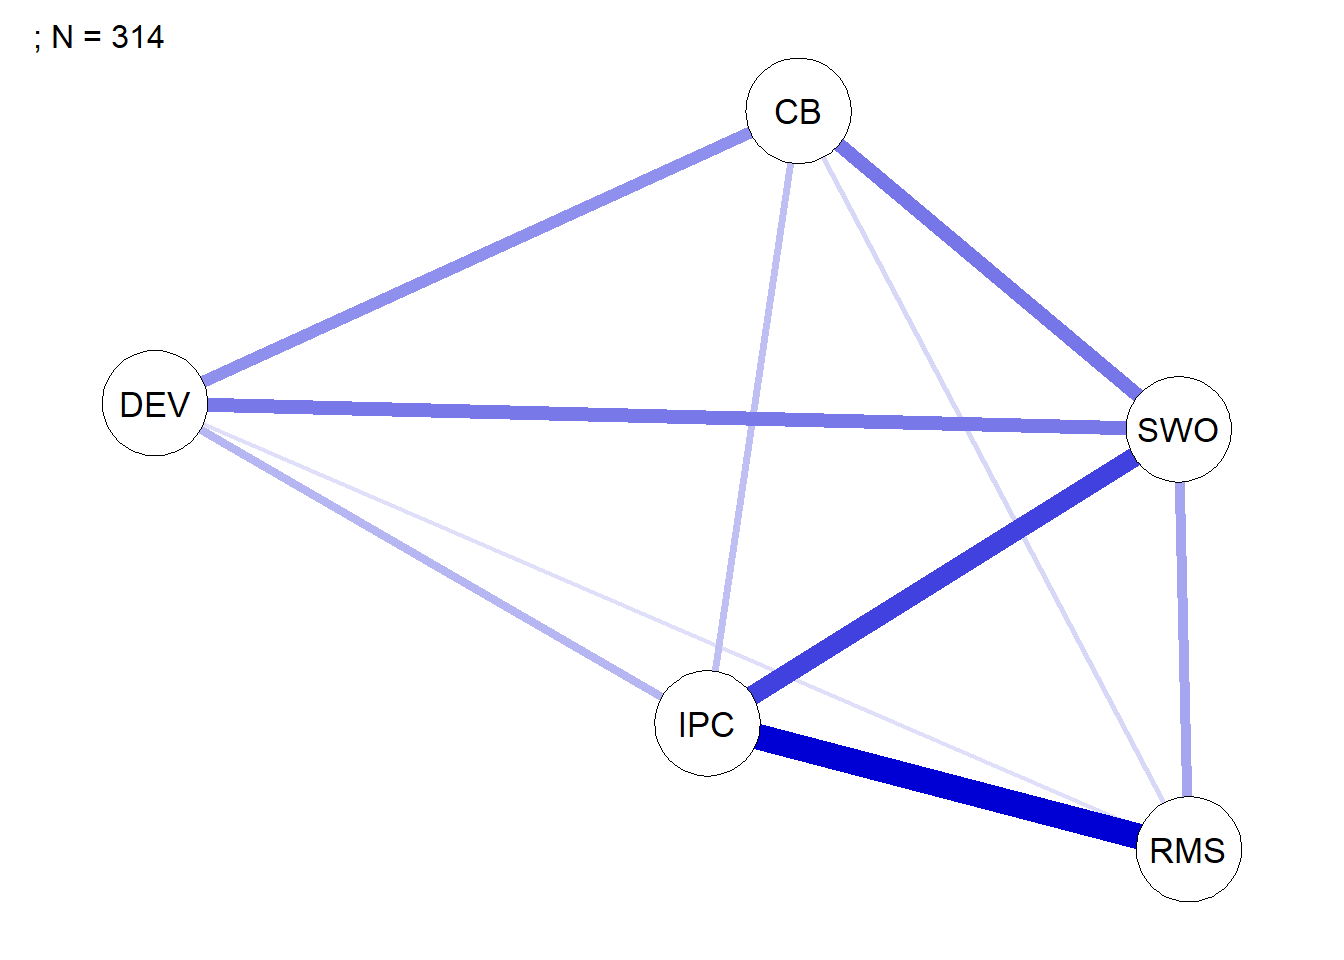
\includegraphics{2021_IDDC_Final-Report_Group-7_files/figure-latex/unnamed-chunk-35-1.pdf}

\begin{center}\rule{0.5\linewidth}{0.5pt}\end{center}

\hypertarget{multinomial-prediction}{%
\section{Multinomial Prediction}\label{multinomial-prediction}}

\hypertarget{examining-regression-features}{%
\subsection{Examining regression
features}\label{examining-regression-features}}

\begin{Shaded}
\begin{Highlighting}[]
\CommentTok{# Construct wide data frame to fit a multinomial model}
\NormalTok{data_multinom <-}\StringTok{ }\NormalTok{data_wide }\OperatorTok\StringTok{ }
\StringTok{  }\KeywordTok{mutate}\NormalTok{(}
    \DataTypeTok{Specialization =} \KeywordTok{relevel}\NormalTok{(}\KeywordTok{as.factor}\NormalTok{(Specialization), }\DataTypeTok{ref =} \StringTok{"Spec Klinische Psychologie"}\NormalTok{)}
\NormalTok{  ) }\OperatorTok\StringTok{ }
\StringTok{  }\KeywordTok{left_join}\NormalTok{(}
\NormalTok{    data }\OperatorTok
\StringTok{      }\KeywordTok{select}\NormalTok{(student_id, cohort),}
    \DataTypeTok{by =} \KeywordTok{c}\NormalTok{(}\DataTypeTok{ID =} \StringTok{"student_id"}\NormalTok{)}
\NormalTok{  ) }\OperatorTok\StringTok{ }
\StringTok{  }\KeywordTok{select}\NormalTok{(}\OperatorTok{-}\NormalTok{ID)}

\CommentTok{# Order alphabetically}
\NormalTok{spec_order <-}\StringTok{ }\NormalTok{data_multinom}\OperatorTok{$}\NormalTok{Specialization }\OperatorTok
\StringTok{  }\KeywordTok{unique}\NormalTok{() }\OperatorTok
\StringTok{  }\KeywordTok{as.character}\NormalTok{()}

\CommentTok{# add features to data }
\NormalTok{data_multinom_feature <-}\StringTok{ }\NormalTok{data_multinom}
\NormalTok{feature_matrix <-}\StringTok{ }\KeywordTok{matrix}\NormalTok{(}\OtherTok{NA}\NormalTok{, }\DataTypeTok{nrow =} \KeywordTok{nrow}\NormalTok{(data_multinom), }\DataTypeTok{ncol =} \DecValTok{3}\NormalTok{)}
\NormalTok{feature_matrix[,}\DecValTok{1}\NormalTok{] <-}\StringTok{ }\KeywordTok{apply}\NormalTok{(data_multinom[,}\DecValTok{2}\OperatorTok{:}\DecValTok{6}\NormalTok{],}\DecValTok{1}\NormalTok{, max)}
\NormalTok{feature_matrix[,}\DecValTok{2}\NormalTok{] <-}\StringTok{ }\KeywordTok{apply}\NormalTok{(data_multinom[,}\DecValTok{2}\OperatorTok{:}\DecValTok{6}\NormalTok{],}\DecValTok{1}\NormalTok{, min)}
\NormalTok{feature_matrix[,}\DecValTok{3}\NormalTok{] <-}\StringTok{ }\KeywordTok{apply}\NormalTok{(data_multinom[,}\DecValTok{2}\OperatorTok{:}\DecValTok{6}\NormalTok{],}\DecValTok{1}\NormalTok{, mean)}
\NormalTok{data_multinom_feature <-}\StringTok{ }\KeywordTok{cbind}\NormalTok{(data_multinom_feature, feature_matrix)}

\CommentTok{# Fit the multinomial feature data only on data from the 1718 cohort }
\NormalTok{fitted_}\DecValTok{1718}\NormalTok{_features <-}\StringTok{ }\KeywordTok{multinom}\NormalTok{(Specialization }\OperatorTok{~}\StringTok{ }\NormalTok{., }\DataTypeTok{data =}\NormalTok{ data_multinom_feature }\OperatorTok\StringTok{ }\KeywordTok{filter}\NormalTok{(cohort }\OperatorTok{==}\StringTok{ "1718"}\NormalTok{) }\OperatorTok\StringTok{ }\KeywordTok{select}\NormalTok{(}\OperatorTok{-}\NormalTok{cohort))}
\end{Highlighting}
\end{Shaded}

\begin{verbatim}
## # weights:  70 (54 variable)
## initial  value 1965.369251 
## iter  10 value 1484.290704
## iter  20 value 1442.409358
## iter  30 value 1439.095692
## iter  40 value 1438.616720
## iter  50 value 1438.592696
## iter  50 value 1438.592689
## iter  50 value 1438.592689
## final  value 1438.592689 
## converged
\end{verbatim}

\begin{Shaded}
\begin{Highlighting}[]
\CommentTok{# Try to predict the 1819 cohort we're using the raw probabilities here}
\CommentTok{# because assigning to the highest probability will}
\CommentTok{# always pick the clinical specialization}
\NormalTok{prediction <-}\StringTok{ }\KeywordTok{predict}\NormalTok{(fitted_}\DecValTok{1718}\NormalTok{_features, }\DataTypeTok{newdata =}\NormalTok{ data_multinom_feature }\OperatorTok\StringTok{ }\KeywordTok{filter}\NormalTok{(cohort }\OperatorTok{==}\StringTok{ "1819"}\NormalTok{) }\OperatorTok\StringTok{ }\KeywordTok{select}\NormalTok{(}\OperatorTok{-}\NormalTok{cohort), }\DataTypeTok{type =} \StringTok{"probs"}\NormalTok{)}

\CommentTok{# Get predicted fraction of people}
\NormalTok{frac_prediction <-}\StringTok{ }\NormalTok{prediction }\OperatorTok
\StringTok{  }\KeywordTok{colMeans}\NormalTok{(}\DataTypeTok{na.rm =}\NormalTok{ T) }

\CommentTok{# Get observed fraction of people for 1718}
\NormalTok{frac_}\DecValTok{1718}\NormalTok{ <-}\StringTok{ }\NormalTok{data }\OperatorTok
\StringTok{  }\KeywordTok{distinct}\NormalTok{(student_id, }\DataTypeTok{.keep_all =}\NormalTok{ T) }\OperatorTok
\StringTok{  }\KeywordTok{select}\NormalTok{(specialisation, cohort) }\OperatorTok\StringTok{ }
\StringTok{  }\KeywordTok{filter}\NormalTok{(cohort }\OperatorTok{==}\StringTok{ "1718"}\NormalTok{) }\OperatorTok\StringTok{ }
\StringTok{  }\KeywordTok{count}\NormalTok{(specialisation) }\OperatorTok\StringTok{ }
\StringTok{  }\KeywordTok{mutate}\NormalTok{(}\DataTypeTok{freq =}\NormalTok{ n }\OperatorTok{/}\StringTok{ }\KeywordTok{sum}\NormalTok{(n)) }\OperatorTok
\StringTok{  }\KeywordTok{pull}\NormalTok{(freq, }\DataTypeTok{name =}\NormalTok{ specialisation)}

\CommentTok{# Get observed fraction of people for 1819}
\NormalTok{frac_}\DecValTok{1819}\NormalTok{ <-}\StringTok{ }\NormalTok{data }\OperatorTok
\StringTok{  }\KeywordTok{distinct}\NormalTok{(student_id, }\DataTypeTok{.keep_all =}\NormalTok{ T) }\OperatorTok
\StringTok{  }\KeywordTok{select}\NormalTok{(specialisation, cohort) }\OperatorTok\StringTok{ }
\StringTok{  }\KeywordTok{filter}\NormalTok{(cohort }\OperatorTok{==}\StringTok{ "1819"}\NormalTok{) }\OperatorTok\StringTok{ }
\StringTok{  }\KeywordTok{count}\NormalTok{(specialisation) }\OperatorTok\StringTok{ }
\StringTok{  }\KeywordTok{mutate}\NormalTok{(}\DataTypeTok{freq =}\NormalTok{ n }\OperatorTok{/}\StringTok{ }\KeywordTok{sum}\NormalTok{(n)) }\OperatorTok
\StringTok{  }\KeywordTok{pull}\NormalTok{(freq, }\DataTypeTok{name =}\NormalTok{ specialisation)}

\CommentTok{# Examine prediction accuracy via correlations}
\KeywordTok{paste}\NormalTok{(}\StringTok{"Correlation using last year's proportions:"}\NormalTok{, }\KeywordTok{cor}\NormalTok{(frac_}\DecValTok{1718}\NormalTok{[spec_order], frac_}\DecValTok{1819}\NormalTok{[spec_order]))}
\end{Highlighting}
\end{Shaded}

\begin{verbatim}
## [1] "Correlation using last year's proportions: 0.947149877476863"
\end{verbatim}

\begin{Shaded}
\begin{Highlighting}[]
\KeywordTok{paste}\NormalTok{(}\StringTok{"Correlation using multinomial predictions:"}\NormalTok{, }\KeywordTok{cor}\NormalTok{(frac_prediction[spec_order], frac_}\DecValTok{1819}\NormalTok{[spec_order]))}
\end{Highlighting}
\end{Shaded}

\begin{verbatim}
## [1] "Correlation using multinomial predictions: 0.934670499519659"
\end{verbatim}

\begin{Shaded}
\begin{Highlighting}[]
\CommentTok{# Examine raw prediction accuracy and visualise it in a plot}
\KeywordTok{data.frame}\NormalTok{(}
  \DataTypeTok{specialisation =}\NormalTok{ spec_order,}
  \DataTypeTok{Correct =}\NormalTok{ frac_}\DecValTok{1819}\NormalTok{[spec_order],}
  \DataTypeTok{Predicted =}\NormalTok{ frac_prediction[spec_order],}
  \DataTypeTok{Last_Year =}\NormalTok{ frac_}\DecValTok{1718}\NormalTok{[spec_order]}
\NormalTok{) }\OperatorTok
\StringTok{  }\KeywordTok{pivot_longer}\NormalTok{(}\OperatorTok{-}\NormalTok{specialisation) }\OperatorTok\StringTok{ }
\StringTok{  }\KeywordTok{ggplot}\NormalTok{(}\KeywordTok{aes}\NormalTok{(}\DataTypeTok{x =} \KeywordTok{factor}\NormalTok{(name, }\DataTypeTok{levels =} \KeywordTok{c}\NormalTok{(}\StringTok{"Last_Year"}\NormalTok{, }\StringTok{"Predicted"}\NormalTok{, }\StringTok{"Correct"}\NormalTok{)), }\DataTypeTok{y =}\NormalTok{ value, }\DataTypeTok{fill =}\NormalTok{ specialisation)) }\OperatorTok{+}
\StringTok{    }\KeywordTok{geom_bar}\NormalTok{(}\DataTypeTok{position =} \StringTok{"fill"}\NormalTok{, }\DataTypeTok{stat =} \StringTok{"identity"}\NormalTok{) }\OperatorTok{+}
\StringTok{    }\KeywordTok{theme_minimal}\NormalTok{() }\OperatorTok{+}
\StringTok{    }\KeywordTok{labs}\NormalTok{(}
      \DataTypeTok{x =} \OtherTok{NULL}\NormalTok{,}
      \DataTypeTok{y =} \StringTok{"Fraction of Students"}\NormalTok{,}
      \DataTypeTok{fill =} \StringTok{"Specialisation"}
\NormalTok{    )}
\end{Highlighting}
\end{Shaded}

\includegraphics{2021_IDDC_Final-Report_Group-7_files/figure-latex/unnamed-chunk-36-1.pdf}

\hypertarget{evaluation-of-multinomial-performance}{%
\subsection{Evaluation of multinomial
performance}\label{evaluation-of-multinomial-performance}}

\begin{Shaded}
\begin{Highlighting}[]
\CommentTok{# Fit the multinomial only on data from the 1718 cohort}
\NormalTok{fitted_}\DecValTok{1718}\NormalTok{ <-}\StringTok{ }\KeywordTok{multinom}\NormalTok{(Specialization }\OperatorTok{~}\StringTok{ }\NormalTok{., }\DataTypeTok{data =}\NormalTok{ data_multinom }\OperatorTok\StringTok{ }\KeywordTok{filter}\NormalTok{(cohort }\OperatorTok{==}\StringTok{ "1718"}\NormalTok{) }\OperatorTok\StringTok{ }\KeywordTok{select}\NormalTok{(}\OperatorTok{-}\NormalTok{cohort))}
\end{Highlighting}
\end{Shaded}

\begin{verbatim}
## # weights:  49 (36 variable)
## initial  value 1965.369251 
## iter  10 value 1584.171278
## iter  20 value 1472.936581
## iter  30 value 1467.481985
## iter  40 value 1467.380019
## final  value 1467.379677 
## converged
\end{verbatim}

\begin{Shaded}
\begin{Highlighting}[]
\CommentTok{# Try to predict the 1819 cohort we're using the raw probabilities here}
\CommentTok{# because assigning to the highest probability will}
\CommentTok{# always pick the clinical specialization}
\NormalTok{prediction <-}\StringTok{ }\KeywordTok{predict}\NormalTok{(fitted_}\DecValTok{1718}\NormalTok{, }\DataTypeTok{newdata =}\NormalTok{ data_multinom }\OperatorTok\StringTok{ }\KeywordTok{filter}\NormalTok{(cohort }\OperatorTok{==}\StringTok{ "1819"}\NormalTok{) }\OperatorTok\StringTok{ }\KeywordTok{select}\NormalTok{(}\OperatorTok{-}\NormalTok{cohort), }\DataTypeTok{type =} \StringTok{"probs"}\NormalTok{)}

\CommentTok{# Get predicted fraction of people}
\NormalTok{frac_prediction <-}\StringTok{ }\NormalTok{prediction }\OperatorTok
\StringTok{  }\KeywordTok{colMeans}\NormalTok{(}\DataTypeTok{na.rm =}\NormalTok{ T) }

\CommentTok{# Get observed fraction of people for 1718}
\NormalTok{frac_}\DecValTok{1718}\NormalTok{ <-}\StringTok{ }\NormalTok{data }\OperatorTok
\StringTok{  }\KeywordTok{distinct}\NormalTok{(student_id, }\DataTypeTok{.keep_all =}\NormalTok{ T) }\OperatorTok
\StringTok{  }\KeywordTok{select}\NormalTok{(specialisation, cohort) }\OperatorTok\StringTok{ }
\StringTok{  }\KeywordTok{filter}\NormalTok{(cohort }\OperatorTok{==}\StringTok{ "1718"}\NormalTok{) }\OperatorTok\StringTok{ }
\StringTok{  }\KeywordTok{count}\NormalTok{(specialisation) }\OperatorTok\StringTok{ }
\StringTok{  }\KeywordTok{mutate}\NormalTok{(}\DataTypeTok{freq =}\NormalTok{ n }\OperatorTok{/}\StringTok{ }\KeywordTok{sum}\NormalTok{(n)) }\OperatorTok
\StringTok{  }\KeywordTok{pull}\NormalTok{(freq, }\DataTypeTok{name =}\NormalTok{ specialisation)}

\CommentTok{# Get observed fraction of people for 1819}
\NormalTok{frac_}\DecValTok{1819}\NormalTok{ <-}\StringTok{ }\NormalTok{data }\OperatorTok
\StringTok{  }\KeywordTok{distinct}\NormalTok{(student_id, }\DataTypeTok{.keep_all =}\NormalTok{ T) }\OperatorTok
\StringTok{  }\KeywordTok{select}\NormalTok{(specialisation, cohort) }\OperatorTok\StringTok{ }
\StringTok{  }\KeywordTok{filter}\NormalTok{(cohort }\OperatorTok{==}\StringTok{ "1819"}\NormalTok{) }\OperatorTok\StringTok{ }
\StringTok{  }\KeywordTok{count}\NormalTok{(specialisation) }\OperatorTok\StringTok{ }
\StringTok{  }\KeywordTok{mutate}\NormalTok{(}\DataTypeTok{freq =}\NormalTok{ n }\OperatorTok{/}\StringTok{ }\KeywordTok{sum}\NormalTok{(n)) }\OperatorTok
\StringTok{  }\KeywordTok{pull}\NormalTok{(freq, }\DataTypeTok{name =}\NormalTok{ specialisation)}

\CommentTok{# Examine prediction accuracy via correlations}
\KeywordTok{paste}\NormalTok{(}\StringTok{"Correlation using last year's proportions:"}\NormalTok{, }\KeywordTok{cor}\NormalTok{(frac_}\DecValTok{1718}\NormalTok{[spec_order], frac_}\DecValTok{1819}\NormalTok{[spec_order]))}
\end{Highlighting}
\end{Shaded}

\begin{verbatim}
## [1] "Correlation using last year's proportions: 0.947149877476863"
\end{verbatim}

\begin{Shaded}
\begin{Highlighting}[]
\KeywordTok{paste}\NormalTok{(}\StringTok{"Correlation using multinomial predictions:"}\NormalTok{, }\KeywordTok{cor}\NormalTok{(frac_prediction[spec_order], frac_}\DecValTok{1819}\NormalTok{[spec_order]))}
\end{Highlighting}
\end{Shaded}

\begin{verbatim}
## [1] "Correlation using multinomial predictions: 0.931448085715915"
\end{verbatim}

\begin{Shaded}
\begin{Highlighting}[]
\CommentTok{# Examine raw prediction accuracy and visualise it in a plot}
\KeywordTok{data.frame}\NormalTok{(}
  \DataTypeTok{specialisation =}\NormalTok{ spec_order,}
  \DataTypeTok{Correct =}\NormalTok{ frac_}\DecValTok{1819}\NormalTok{[spec_order],}
  \DataTypeTok{Predicted =}\NormalTok{ frac_prediction[spec_order],}
  \DataTypeTok{Last_Year =}\NormalTok{ frac_}\DecValTok{1718}\NormalTok{[spec_order]}
\NormalTok{) }\OperatorTok
\StringTok{  }\KeywordTok{pivot_longer}\NormalTok{(}\OperatorTok{-}\NormalTok{specialisation) }\OperatorTok\StringTok{ }
\StringTok{  }\KeywordTok{ggplot}\NormalTok{(}\KeywordTok{aes}\NormalTok{(}\DataTypeTok{x =} \KeywordTok{factor}\NormalTok{(name, }\DataTypeTok{levels =} \KeywordTok{c}\NormalTok{(}\StringTok{"Last_Year"}\NormalTok{, }\StringTok{"Predicted"}\NormalTok{, }\StringTok{"Correct"}\NormalTok{)), }\DataTypeTok{y =}\NormalTok{ value, }\DataTypeTok{fill =}\NormalTok{ specialisation)) }\OperatorTok{+}
\StringTok{    }\KeywordTok{geom_bar}\NormalTok{(}\DataTypeTok{position =} \StringTok{"fill"}\NormalTok{, }\DataTypeTok{stat =} \StringTok{"identity"}\NormalTok{) }\OperatorTok{+}
\StringTok{    }\KeywordTok{theme_minimal}\NormalTok{() }\OperatorTok{+}
\StringTok{    }\KeywordTok{labs}\NormalTok{(}
      \DataTypeTok{x =} \OtherTok{NULL}\NormalTok{,}
      \DataTypeTok{y =} \StringTok{"Fraction of Students"}\NormalTok{,}
      \DataTypeTok{fill =} \StringTok{"Specialisation"}
\NormalTok{    )}
\end{Highlighting}
\end{Shaded}

\includegraphics{2021_IDDC_Final-Report_Group-7_files/figure-latex/multinom_eval-1.pdf}

\end{document}
